% Chapter 1
   
\chapter{Elementos de Demograf\'ia y Teor\'ias de la Poblaci\'on} % Main chapter title

\hspace{9cm}\textit{``Life is... a chemical incident''} -- Paul Ehrlich}

\label{Chapter1} % For referencing the chapter elsewhere, use \ref{Chapter1} 

%----------------------------------------------------------------------------------------

% Define some commands to keep the formatting separated from the content 
\newcommand{\keyword}[1]{\textbf{#1}}
\newcommand{\tabhead}[1]{\textbf{#1}}
\newcommand{\code}[1]{\texttt{#1}}
\newcommand{\file}[1]{\texttt{\bfseries#1}}
\newcommand{\option}[1]{\texttt{\itshape#1}}

%----------------------------------------------------------------------------------------
\section{Introducci\'on: motivaci\'on, objetivos, estructura y metodolog\'ia del trabajo}

El mundo envejece. Quiz\'a no es la mejor forma, o al menos no parece la m\'as optimista, para comenzar un trabajo de esta \'indole, pero lo cierto es que es as\'i. Es as\'i porque los datos lo demuestran.\\

El mundo envejece tanto en el plano individual como poblacional. Como individuos, vivimos cada vez m\'as. La esperanza de vida al nacer se ha incrementado en el plano global, pasando de 47 a\~nos a mediados del siglo pasado a alrededor de 71 a\~nos hoy en d\'ia y se espera que llegue a 78 a\~nos a mediados del presente siglo. Como población tambi\'en estamos envejeciendo, ya que cada vez son m\'as amplias las franjas demogr\'aficas de mayor edad. Actualmente, la proporci\'on de la poblaci\'on mundial con 65 o m\'as a\~nos es alrededor de un 8\% y se espera que en el 2050 llegue a un 16\%, lo cual supondr\'a m\'as de 1.500 millones de personas.\\

En Espa\~na tenemos una de las mayores longevidades del mundo, bajas tasas de natalidad y un problema de desempleo que hace que la tasa de actividad sea baja. Por ejemplo, en este momento, por cada jubilado hay 2,2 cotizantes y todo apunta, a que en 2050, la proporci\'on bajar\'a a 1,3 cotizantes por jubilado. Ante este panorama, la \textbf{motivaci\'on} de esta tesis surge como consecuencia del planteamiento de la siguiente pregunta: \textit{?`c\'omo planificamos nuestra jubilaci\'on en la era de la longevidad?} Las pensiones, el futuro de las mismas o de forma m\'as precisa, el futuro de la nuestra, es un tema que interesa a todos. Es patente que los espa\~noles estamos cada vez m\'as preocupados por c\'omo financiaremos nuestra jubilaci\'on si las pensiones siguen reduci\'endose. Sin embargo, nos ocupamos poco de planificar esta etapa.\\

Por ello, con la pregunta formulada anteriormente como premisa inicial y como idea central de esta tesis, se persiguen, adicionalmente, varios \textbf{objetivos}: por un lado, reflejar la situaci\'on demogr\'afica mundial en la actualidad y, en concreto, de Espa\~na, analizando sus consecuencias económicas, sociales y geopol\'iticas (con especial atenci\'on a la influencia que tiene la situaci\'on demogr\'afica actual en los sistemas de pensiones) y por otro, plantear el problema de la planificaci\'on financiera a largo plazo, presentando una serie de recursos disponibles y, en última instancia, analizando la figura de la hipoteca inversa como complemento a una pensi\'on por jubilaci\'on que empieza a ser insuficiente para cubrir las necesidades de la tercera edad.\\

La presente tesis \textbf{se estructura en siete cap\'itulos, más uno adicional a modo de cierre y conclusiones}, agrupados en dos partes; un \textbf{primer bloque} donde se desarrollan aspectos te\'oricos relacionados con la demograf\'ia y las pensiones. Esta parte creemos que es necesaria porque la comprensi\'on de los fen\'omenos demogr\'aficos nos da una perspectiva más amplia a la hora de explicar la situaci\'on en la que nos encontramos y nos sitúa en una posición privilegiada para entender c\'omo se ha llegado hasta aqu\'i como para tener que preocuparnos por c\'omo viviremos cuando envejezcamos. Consta de cuatro cap\'itulos: en el \textbf{primero} de ellos, titulado \textit{``Elementos de Demograf\'ia y Teor\'ias de la Poblaci\'on''}, se describen los principales fen\'omenos demogr\'aficos a la hora de estudiar la misma, se explica el actual `boom' demogr\'afico mundial y se enumeran los problemas m\'as importantes a los que nos enfrentamos -individuos e instituciones- como habitantes de un planeta cada vez m\'as poblado y envejecido; seguidamente, se analizan las consecuencias sociales y geopol\'iticas del crecimiento y del envejecimiento de la poblaci\'on, para pasar a revisar y analizar, posteriormente, en el  cap\'itulo \textbf{segundo}, que lleva por título \textit{``Métodos de Análisis de los Fenómenos Demográficos''}, algunos de los modelos estoc\'asticos proyección de la fertilidad y de la mortalidad m\'as conocidos y su aplicación, en nuestro caso, a la población española.\\

Estos dos primeros cap\'itulos implican el estudio tanto de instrumentos de an\'alisis como de procedimientos estad\'isticos, aunque sin dejar de lado el procedimiento explicativo, pues de lo que se trata principalmente es de ofrecer una visi\'on sistem\'atica de una ciencia social, la demograf\'ia, ligada de forma muy estrecha a otras ramas del saber, lo cual no est\'a exento de dificultad, ya que el desarrollo en los \'ultimos sesenta a\~nos de esta disciplina ha provocado que exista una demograf\'ia econ\'omica, una antropolog\'ia demogr\'afica, una demograf\'ia m\'edica..., etc., todas con sus correspondientes procedimientos de an\'alisis y medici\'on. Este hecho no hemos querido perderlo de vista y por ello algunos de los conceptos, definiciones, técnicas y simulaciones aquí propuestos podrían pertenecer perfectamente a alguna de las sub-disciplinas mencionadas antes.\\

En el cap\'itulo \textbf{tercero}, \textit{``Los Sistemas de Pensiones: Un Recorrido Mundial''}, se explica qu\'e es un sistema de pensiones, se realiza un recorrido por los de los pa\'ises mejor valorados conforme a un índice que compara adecuación, sostenibilidad e integridad y se plantea la sostenibilidad actual de dichos sistemas y las reformas que habr\'ian de ser acometidas para garantizar esa sostenibilidad.\\

En el cap\'itulo \textbf{cuarto}, \textit{``Aspectos T\'ecnicos de los Sistemas de Pensiones''}, se aborda la cuestión desde un punto de vista actuarial. La importancia de este capítulo radica en que esta visión permite comprender el problema al que se enfrentan los responsables tanto de entes públicos (gobiernos e instituciones) como privados (aseguradoras, bancos, etc...) a la hora de manejar el riesgo y la incertidumbre asociados a la longevidad, desde un punto de vista actuarial y financiero.\\

En el \textbf{quinto} cap\'itulo, \textit{``El Caso Español''}, nos centramos ya en nuestro país, comenzando con un recorrido hist\'orico en el que se hace referencia a los primeros sistemas de protecci\'on de la vejez que comienzan en 1939 y contin\'ua con la evoluci\'on de la Seguridad Social hasta llegar al actual sistema de pensiones contributivas de nuestros d\'ias, donde se analizar\'a la \'ultima reforma llevada a cabo. Para finalizar el cap\'itulo, y al igual que el anterior, se plantearán los principales problemas a los que nos enfrentamos ahora y en el futuro, así como el debate de la sostenibilidad del mismo y las propuestas de reformas que habr\'ia que llevar a cabo para la supervivencia del sistema a medio y largo plazo.\\ %comenzando por su situaci\'on demogr\'afica actual, se describen los principales problemas a los que nos enfrentamos ahora y en el futuro, para continuar analizando nuestro sistema de pensiones, ello se realiza

El \textbf{segundo bloque} desarrolla la parte pr\'actica de esta tesis a través de los dos capítulos que abarca. En el \textbf{sexto}, \textit{``Aspectos Prácticos Para la Planificación de la Jubilación''}, se recogen diversos aspectos prácticos a la hora de planificar la misma, para ello se proporcionan unos principios básicos en el aspecto financiero, indicando cuándo y cómo sería más conveniente ahorrar para cuando llegue el retiro, en un intento de proporcionar las herramientas básicas que todo individuo debería conocer. Asimismo se ha diseñado una pequeña aplicación informática en código \textsf{\textbf{R}} que permite generar retornos aleatorios simulando diferentes tipos de interés, niveles de inflación, rentabilidades exigidas y cantidades iniciales a invertir. \\

El cap\'itulo \textbf{siete}, \textit{``La Hipoteca Inversa''}, es el que termina por completar el último objetivo que nos planteamos ya que aquí es donde se ofrece este producto financiero como alternativa real para obtener un ingreso adicional y poder complementar así la pensión. Es un producto que por las razones que veremos no ha calado profundamente en nuestro país pero se analiza detenidamente y se estudia en profundidad sus características, ventajas e inconvenientes, se configura como una alternativa válida a otros productos financieros con un elevado componente de riesgo e incertidumbre o con unos rendimientos más bajos.\\

El \textbf{octavo} capítulo cierra la obra recogiendo las conclusiones finales a las que hemos llegado durante lo expuesto en todas las partes previas y si bien al final de todos los apartados anteriores ya se habían expuesto unos argumentos a modo de cierre, esta sección pretende ser un compendio global de todo lo visto anteriormente.\\

Para finalizar, se incluyen unos \textbf{anexos y apéndices} que son necesarios, a nuestro juicio, para complementar ciertos análisis y aspectos tratados en algunos capítulos. De este modo, por ejemplo, hemos pensado que podría ser interesante incluir un breve diccionario demográfico que ayude al lector a clarificar algunos conceptos en esta materia; de igual modo, se ha creído conveniente especificar la notación actuarial estándar comúnmente aceptada y asimismo, hemos considerado necesario adjuntar los \textit{`scripts'} y códigos utilizados en \textsf{\textbf{R}} para nuestras simulaciones, modelos y gráficos, siguiendo la propia filosofía característica de los programas de código abierto.\\

En referencia a las partes más cuantitativas o puramente de modelización y simulación, la \textbf{metodología} aplicada, tanto de desarrollo de modelos como de simulaciones, ha estado basada en el uso de herramientas del campo de la estadística, principalmente y como se ha mencionado con anterioridad, todo ha sido desarrollado con el software \textsf{\textbf{R}}. El uso de este programa de código abierto ha sido por varios motivos: primero por su versatilidad y potencia, el hecho de que sea de código abierto \textit{(`open source')} lo hace fácilmente adaptable y flexible a cualquier tipo de análisis, siendo una herramienta muy potente para todo tipo de procesamiento, manipulación de datos y resultados gráficos; segundo porque el uso principal que se le suele dar es con fines estadísticos y este trabajo es, en gran medida, estadístico y de simulación y tercero porque esa versatilidad que mencionábamos antes se traduce en la existencia de multitud de librerías y paquetes que son de acceso público y aumentan la eficacia de los resultados.\\

Menci\'on aparte merece la \textbf{bibliograf\'ia} utilizada. Primero, porque la hemos adjuntado al final de cada capítulo y está citada en orden cronológico (no alfabético) decisión que obedece a una simple cuestión de practicidad, pues de esta manera se considera más accesible y clara, ayudando más a reforzar y complementar cada capítulo, en vez de al final de la obra, lo cual puede resultar, esto último, menos efectivo. Segundo, por su relevancia y actualización, ya que un trabajo de esta índole aparte de beber de muchas fuentes y referencias diversas (todas ellas fundamentales en la elaboración de esta tesis) ha tenido que ser actualizado constantemente, de este modo, las fuentes consultadas van desde libros, tanto clásicos en su materia como de reciente aparición hasta revistas de calidad, informes, art\'iculos t\'ecnicos y bases de datos.\\

Finalmente no hemos querido dejar de lado la vertiente econ\'omica que tiene como trasfondo este trabajo, al final las consecuencias de todo lo anterior se traducen en un coste económico para todos los agentes implicados, desde países, gobiernos, instituciones y empresas hasta familias e individuos y todos ellos, aún con retos diferentes, tienen un objetivo común.

%%%%%%%%%%%%%%%%%%%%%% SECCION 1.2.: FENÓMENOS DEMOGR\'AFICOS %%%%%%%%%%%%%%%%%%%%%%
\newpage

\section{Los fen\'omenos demogr\'aficos: su observaci\'on y an\'alisis}

Las tendencias demogr\'aficas mundiales en la actualidad est\'an contribuyendo a que haya poblaciones cada vez m\'as envejecidas, ya que mientras la esperanza de vida ha crecido de forma constante desde principios del siglo XX y la vida seguir\'a prolong\'andose cada vez m\'as en el futuro, la tasa de natalidad contin\'ua cayendo. La demograf\'ia de los siglos XX y XXI ha sido y es, sobre todo, una demograf\'ia del envejecimiento de la poblaci\'on (Harper, 2016) \textcolor{red}{[1]}. Este hecho, que en otro tiempo se consider\'o un asunto de econom\'ias desarrolladas de Europa y Am\'erica del Norte, es ahora un fen\'omeno global que se extiende por todo el mundo.\\

A principios del siglo XX, en la Tierra viv\'ian alrededor de 1.600 millones de personas; en julio de 1987 se alcanzaron los 5.000 millones; a finales de ese siglo, la poblaci\'on mundial super\'o los 6.000 millones y actualmente es de 7.600 millones de habitantes. En lo que llevamos de siglo, la poblaci\'on ha aumentado en 1.600 millones, es decir, un 27\%. En cien a\~nos, la poblaci\'on mundial ha crecido un 375\%. Seg\'un Sartori y Mazzoleni (2003) \textcolor{red}{[2]}, los dem\'ografos calculan que la tasa de mantenimiento (ni crecimiento ni reducci\'on) coincide con una fertilidad femenina de poco m\'as de dos; es decir, las mujeres deben traer al mundo una media de dos hijos cada una para reemplazarse a s\'i mismas y a los varones. Los autores anteriormente mencionados afirman que esta tasa se aumenta ligeramente para compensar la mortalidad infantil, los que no se casan, no tienen hijos, etc... Si se tiene en cuenta que la din\'amica demogr\'afica europea (sin contar los inmigrantes) est\'a descendiendo y que la poblaci\'on de los Estados Unidos crece sobre todo por la inmigraci\'on (legal y clandestina) procedente de Am\'erica Latina y Asia, se refuerza la idea de que la explosi\'on demogr\'afica se debe en mayor medida, a los pa\'ises africanos y asi\'aticos, es decir, excepto casos espec\'ificos, a las \'areas m\'as pobres y menos desarrolladas.\\ 

A\'un as\'i, ?`quiere esto decir que el mundo est\'a superpoblado? Muchas veces se confunde el t\'ermino `superpoblaci\'on' con `aglomeraci\'on'. Con frecuencia o\'imos expresiones del tipo \textit{``demasiadas personas en una determinada zona'', ``una densidad de poblaci\'on excesivamente elevada''}. Normalmente, la densidad es intrascendente en materia de superpoblaci\'on; por ejemplo, si atendemos al criterio de densidad bruta tenemos las siguientes densidades de poblaci\'on:\footnote{La densidad poblacional viene determinada por el cociente entre el n\'umero de habitantes y la superficie del \'area.}

\begin{table}[h!]
  \begin{center}
    \begin{tabular}{|c|c|c|c|c|} \hline% <-- Alignments: 1st column left, 2nd middle and 3rd right, with vertical lines in between
    \rowcolor{gray!30} & \textbf{Asia} & \textbf{Europa} & \textbf{\'Africa} & \textbf{Jap\'on}\\ \hline
    \'Area (km\textsuperscript{2})  &  44.541.138 & 10.180.000	& 30.370.000 & 377.915\\ \hline
    Poblaci\'on (mill. hab.)  &  4.393.000.000 & 738.199.000 & 1.022.234.000 & 126.926.000\\ \hline
    \rowcolor{gray!30}  Densidad (habs./km\textsuperscript{2}) & \textbf{98,63} & \textbf{72,51} & \textbf{33,66} & \textbf{335,86}\\ \hline
    \end{tabular}
    \caption{Comparativa de densidades de poblaci\'on en 2017}\\
    \textit{(Fuente: Elaboraci\'on propia)}
    \label{tab:table1}
  \end{center}
\end{table}

\vspace{-0.5cm}
Seg\'un lo anterior, llegar\'iamos a la conclusi\'on de que \'Africa est\'a <<subpoblada>>, puesto que s\'olo tiene 33,66 hab./km\textsuperscript{2}, mientras que Europa tiene 72,51 hab./km\textsuperscript{2}, Asia 98,63 hab./km\textsuperscript{2} y Jap\'on 335,86 hab./km\textsuperscript{2}. Si quisi\'eramos ser m\'as precisos, excluir\'iamos del c\'alculo la proporci\'on de \'Africa que es inhabitable, es decir, la que se halla cubierta por desierto o selvas densas e impenetrables, lo cual hace que la proporci\'on m\'as habitable ocupe algo m\'as de la mitad de la superficie del continente, arrojando una densidad demogr\'afica de unos 47 hab./km\textsuperscript{2}. Ello equivale a una sexta parte de la densidad demogr\'afica del Reino Unido, que actualmente es de 269,45 hab./km\textsuperscript{2}, aproximadamente. Por lo tanto, seg\'un Ehrlich, \textit{la clave para comprender el problema de la superpoblaci\'on no est\'a en la densidad de poblaci\'on, sino en el n\'umero de personas que viven en una determinada zona en relaci\'on con sus recursos y con la capacidad del medioambiente para sostener las actividades humanas; es decir, la ``capacidad de carga'' de dicha zona}, (Ehrlich, 2003) \textcolor{red}{[3]}. De este modo, un \'area estar\'ia superpoblada cuando sus ocupantes degradan la capacidad de carga a largo plazo de dicha \'area.\\

El mismo Ehrlich, ya en 1968 \textcolor{red}{[4]}, preve\'ia la muerte por inanici\'on de una cuarta parte de la poblaci\'on mundial en 1983. Dicha fecha estaba equivocada pero quiz\'as no era muy equivocada la previsi\'on sobre los muertos de hambre que iba a haber. Seg\'un Sartori, el argumento que apoyaba este razonamiento era el impacto ambiental del hombre, el cual es producto de tres factores: \textit{1) el n\'umero de habitantes de la Tierra, multiplicado por 2) su renta per c\'apita, multiplicado por 3) el nivel de tecnolog\'ia.}\\

\vspace{-0.2cm}
En esta irrupci\'on demogr\'afica que ha cambiado el mundo, sobre todo, en el \'ultimo siglo y ha modificado, de forma irreversible podr\'iamos decir, las relaciones del hombre con el espacio geogr\'afico, dos son los motores principales del cambio etario estructural de la poblaci\'on: la fecundidad y la mortalidad, y aunque profundizaremos en ellos de forma m\'as cuantitativa en el siguiente cap\'itulo (junto a otros fen\'omenos de igual importancia), hemos cre\'ido conveniente introducirlas en este primer apartado.\\ 

\vspace{-0.2cm}
La \textbf{fecundidad} es el primero de ellos y \'esta ha descendido en todas las regiones del mundo. Durante el desarrollo econ\'omico del siglo XX se produjo un descenso de las tasas de fecundidad debido al incremento de los gastos sociales relacionados con los hijos y los costes de oportunidad de la paternidad responsable. Las teor\'ias econ\'omicas cl\'asicas de la fecundidad otorgan un papel importante a los costes relacionados con los hijos. A medida que aumenta el coste por hijo, disminuye el n\'umero de los mismos; de modo que, a medida que aumenta la renta disponible con el crecimiento econ\'omico, aumentan los costes de oportunidad de tener hijos. Sin embargo, en la actualidad, esta visi\'on, que apoya la correlaci\'on negativa entre crecimiento econ\'omico y fecundidad, se est\'a revisando y se propone \textit{``un impacto convexo del crecimiento econ\'omico sobre los niveles de fecundidad''}, (Leeson, 2018) \textcolor{red}{[5]}.\\

\vspace{-0.2cm}
La \textbf{mortalidad} es el segundo motor del cambio etario estructural. Con el cambio del siglo XIX al XX, la esperanza de vida a los 65 a\~nos empez\'o a crecer de modo constante y gracias a los avances en la higiene y las posibilidades de tratamiento m\'edico (en especial, al desarrollo de los antibi\'oticos), la poblaci\'on mundial ha podido crecer en un modo sin precedentes tras el final de la Segunda Guerra Mundial. Frente a los 2.500 millones de habitantes en torno a 1950, hoy el planeta cuenta con 7.600 millones. La \textbf{figura 1.1} ofrece una panor\'amica de este `boom' demogr\'afico que hemos experimentado en las \'utimas d\'ecadas. Se espera que para el a\~no 2050, la poblaci\'on mundial se incremente un 14\%, pasando a 9.800 millones de habitantes y para finales de siglo, se sit\'ue en 11.200 millones\footnote{Hasta el a\~no 2050 las proyecciones de la ONU se consideran adecuadas. Tambi\'en las anteriores proyecciones han demostrado una alta fiabilidad, como demuestra el cient\'ifico ingl\'es Alan Cottrell: \textit{``Econom\'ia del medio ambiente'', Ed. Alhambra, (1980)}, recordando las proyecciones de 1975 referidas a 2000, cuando la ONU preve\'ia que la poblaci\'on mundial ser\'ia de 6.100 millones en el a\~no 2000, c\'alculo que ha demostrado ser bastante preciso.}. Por regiones, Asia concentra la mayor parte de la poblaci\'on mundial y se prev\'e que lo siga haciendo hasta finales de siglo, aunque el incremento de la poblaci\'on africana ser\'a a un ritmo creciente y entre los dos continentes agrupar\'an a m\'as del 90\% de la poblaci\'on mundial. A niveles de fertilidad mundial, en la actualidad, \'Africa ostenta el mayor n\'umero de hijos nacidos vivos por mujer, alrededor de 4 (en Europa apenas se llega a 2), sin embargo, es una tasa de fertilidad en constante disminuci\'on, de hecho se espera que a finales de siglo, baje hasta casi 2 hijos por mujer, mientras que en Europa se incremente hasta esa cifra.\\

\vspace{-0.2cm}
Por pa\'ises, la mitad del crecimiento mundial se concentra en nueve, y en este orden: China, India, Estados Unidos, Indonesia, Brasil, Pakist\'an, Nigeria, Bangladesh, Rusia. Juntos suman m\'as de 4.200 millones de habitantes, es decir, casi el 56\% de la poblaci\'on mundial se agrupa en estos pa\'ises. A la cabeza, China (1.400 millones) e India (1.300 millones) tienen un 19\% y un 18\% de la poblaci\'on mundial respectivamente. Se estima que hacia 2024, India superar\'a a China, arrebat\'andole el primer puesto y en este orden (primero y segundo) los sit\'uan las proyecciones hasta 2100.\\

\vspace{-0.2cm}
Destacable es el caso de Nigeria, pa\'is que constituye una perfecta yuxtaposici\'on de riqueza y desarrollo junto a una pobreza end\'emica. No en vano, actualmente ocupa el s\'eptimo puesto en la lista de los pa\'ises m\'as poblados, con una poblaci\'on de 191 millones de habitantes; sin embargo, su r\'apido crecimiento hace que se proyecte su ascenso al tercer puesto en el a\~no 2050, donde pasar\'a a tener una poblaci\'on estimada de algo menos de 800 millones de habitantes. Lagos, la capital, ha pasado de ser una ciudad portuaria muy pobre a ser una de las aglomeraciones urbanas m\'as grandes y pr\'osperas del continente, con una poblaci\'on de 16 millones de habitantes. Su expansi\'on empez\'o en buena medida durante la d\'ecada de 1990, tras la transici\'on a la democracia del pa\'is. Junto a este factor, jug\'o un papel importante el desarrollo de los campos petrol\'iferos; sin embargo, no es el petr\'oleo el \'unico factor responsable de ese veloz progreso, ya que con frecuencia se subestima el papel que las explotaciones mineras han desempe\~nado en el auge del pa\'is africano.

\newpage
\begin{figure}[!ht]
\vspace{-0.5cm}
%\centering
\hspace*{-1.1cm}
\fbox{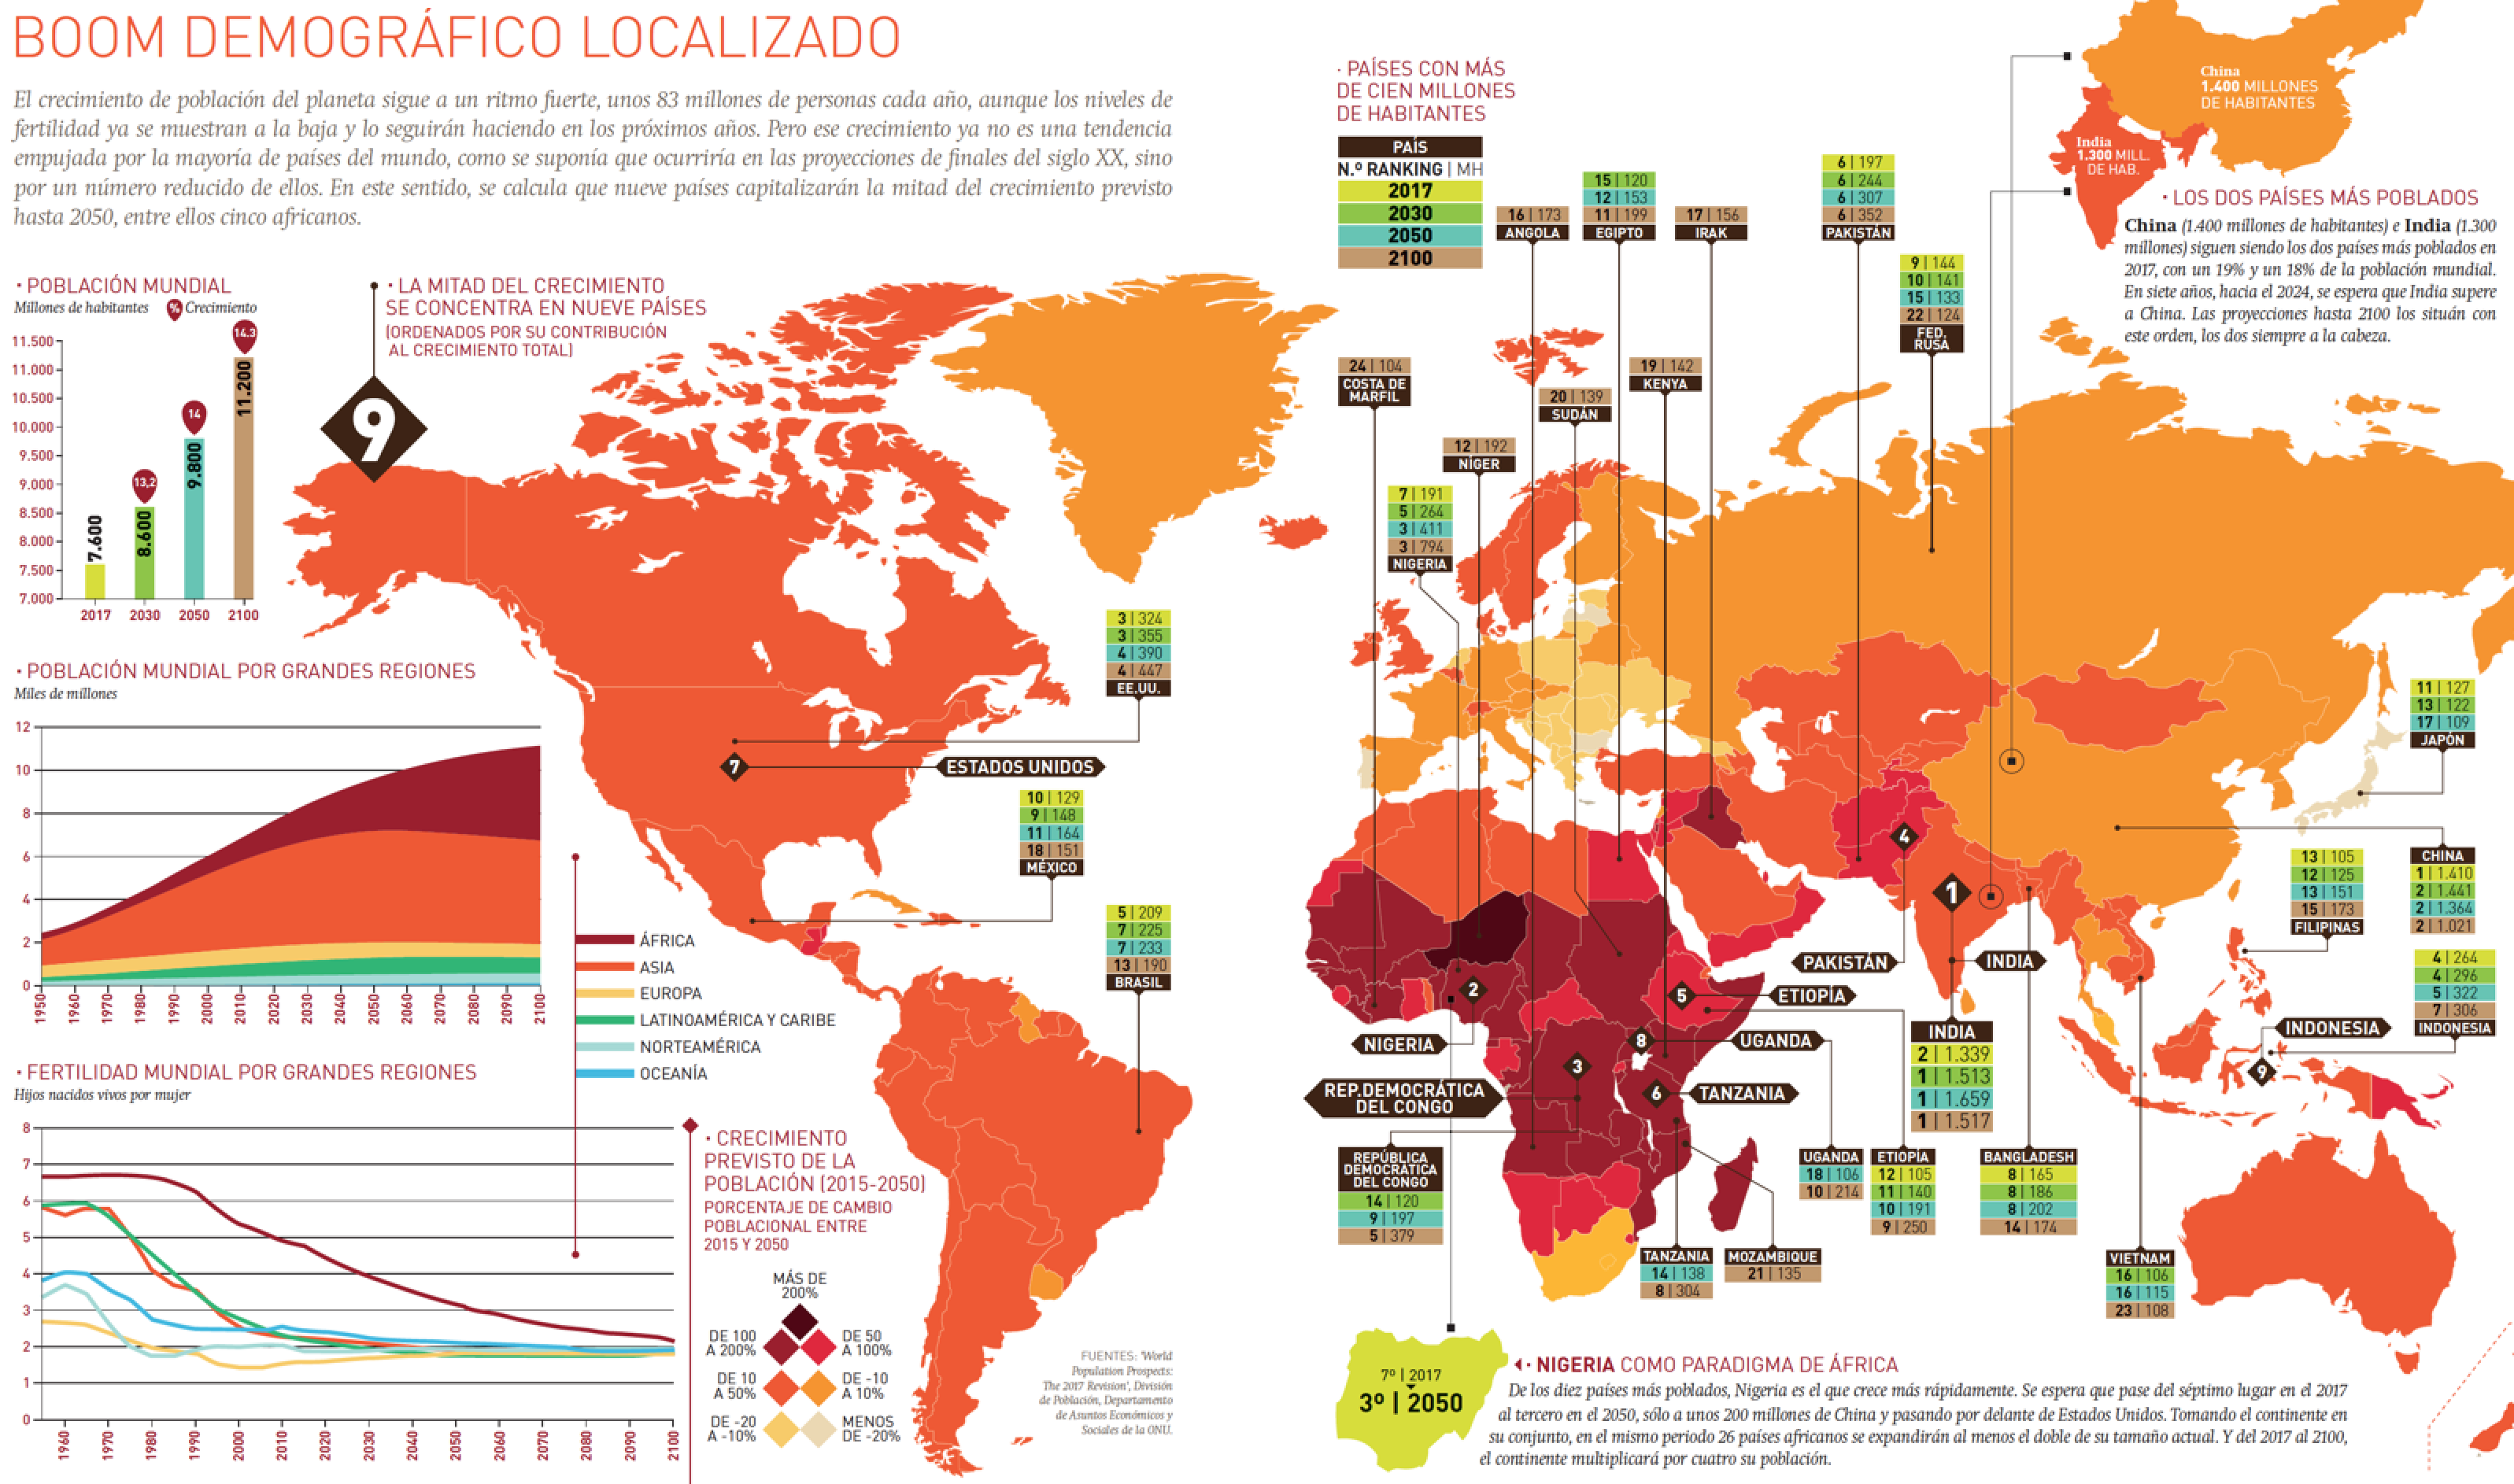
\includegraphics[rotate=90, width=18.7cm,height=24cm]{Cap1/apaisado01.png}}
\caption{Panor\'amica general del boom demogr\'afico mundial}\\
\hspace{2cm}\textit{(Fuentes: World Population Prospects y Dpto. Asuntos Econ\'omicos y Sociales ONU)}
\end{figure}

Seg\'un Kashnitsky y Sch\"oley, 2018 \textcolor{red}{[6]}, el envejecimiento no se trata exclusivamente del tama\~no de la poblaci\'on anciana o su proporci\'on de poblaci\'on; el envejecimiento es una funci\'on de la distribuci\'on por edades de una poblaci\'on. Por lo tanto, para comprender mejor el envejecimiento, hay que centrarse en la evoluci\'on de la estructura de edad de toda la poblaci\'on. Seg\'un esto, en la \textbf{figura 1.2}, los autores muestran la estructura por edades codificada por colores de las regiones europeas, indicando las distintas etapas del envejecimiento de la poblaci\'on en toda Europa y proporcionando una instant\'anea detallada de todas las estructuras de la poblaci\'on regional, facilitando las comparaciones entre ellas. De este modo, se observa que el proceso de envejecimiento de la poblaci\'on no se produce uniformemente en todas las \'areas de Europa y las regiones difieren sustancialmente, as\'i, podemos ver las diferencias regionales a peque\~na y gran escala en las estructuras de la poblaci\'on. En el nivel macro, las distinciones entre el este, el oeste y el sur de Europa son evidentes. El este de Turqu\'ia es el \'unico ejemplo de una sociedad que todav\'ia se encuentra en las primeras etapas de la transici\'on demogr\'afica. A nivel de pa\'is, los contrastes de la periferia central son obvios. El mapa tambi\'en revela los signos de cambios recientes en las estructuras de la poblaci\'on. Por ejemplo, Espa\~na recibi\'o una gran afluencia de migrantes internacionales en la d\'ecada de 2000, Alemania oriental experiment\'o un efecto agotador de emigraci\'on junto con una disminuci\'on de la fertilidad en las \'ultimas d\'ecadas, y Polonia tuvo una emigraci\'on masiva de trabajadores debido a la integraci\'on de la Uni\'on Europea y m\'as trabajadores migrantes se mudaron de las principales ciudades polacas. 

\begin{figure}[!ht]
\centering
\hspace*{-0.5cm}
\includegraphics[scale=0.04]{Cap1/colorcoded.png}
\caption{Mapa de las estructuras de poblaci\'on en las regiones NUTS-3 en 2015}\\
\textit{(Fuente: Adaptaci\'on propia en R a partir de Kashnitsky y Sch\"oley con datos de Eurostat)}
\end{figure}

En la \textbf{figura 1.3} se muestra que la esperanza de vida masculina al nacer desde 1950 ha ido convergiendo cada vez m\'as, pasando de estar 
dividida en dos, a concentrarse, progresivamente, alrededor de los 70 a\~nos.

\newpage

\begin{figure}[!ht]
\centering
%\hspace*{-1.2cm}
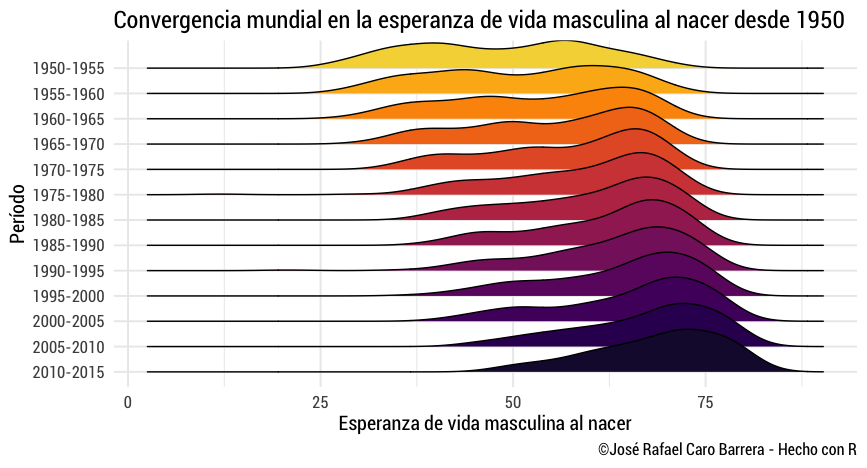
\includegraphics[scale=0.45]{Cap1/convergencia.png}
\caption{Convergencia mundial en la esperanza de vida masculina al nacer desde 1950}\\
\textit{(Fuente: Elaboraci\'on propia a partir de datos extra\'idos de U. N. World Population Prospects 2017 Revision)}
\end{figure}

Si el envejecimiento es el problema demogr\'afico capital del siglo XXI, los \textbf{movimientos migratorios} y la \textbf{urbanizaci\'on} son el segundo problema de ese orden, dado que adem\'as ambos est\'an \'intimamente ligados.\\ 

\vspace{-0.2cm}
La \textit{migraci\'on} es el fen\'omeno demogr\'afico m\'as dif\'icil de observar. Aunque el tema de los fen\'omenos migratorios se abordar\'a cuando tratemos las consecuencias econ\'omicas, sociales y geopol\'iticas de los fen\'omenos demogr\'aficos al final de este cap\'itulo y de forma m\'as cualitativa en el cap\'itulo 2, cuando se analicen los modelos de predicci\'on de los fen\'omenos demogr\'aficos, no podemos pasar por alto el papel que la inmigraci\'on juega en la demograf\'ia y m\'as en concreto, el papel de la migraci\'on `forzosa' ocasionada por las condiciones de vida del pa\'is en cuesti\'on.\\ 

\vspace{-0.2cm}
Casi dos d\'ecadas despu\'es de que la ONU declarara el 18 de diciembre como el \textit{D\'ia Internacional del Migrante}, los problemas de capitalizaci\'on en todo el mundo han llevado a m\'as de 65 millones de personas desplazadas al extranjero o dentro de sus propias fronteras, la mayor cantidad jam\'as registrada por la Comisi\'on de Derechos Humanos de las Naciones Unidas (ACNUR).\\ 

\vspace{-0.2cm}
Pr\'acticamente regiones de todo el mundo sufren movimientos migratorios masivos y \'exodos descontrolados. Las llegadas a trav\'es del Mediterr\'aneo procedentes del norte y del \'Africa subsahariana con destino a pa\'ises como Espa\~na, Italia y Grecia, alcanzaron un m\'aximo en 2015 de m\'as de 1 mill\'on de personas. El gobierno de Italia ha acogido a 650.000 migrantes desde 2014 y es el punto por donde la mayor\'ia de los migrantes todav\'ia cruzan la frontera, principalmente a trav\'es de Libia. En los Estados Unidos, el cruce de la frontera desde Cuba y M\'ejico se cobra una media mensual de entre 20.000 y 40.000 inmigrantes aprehendidos mientras intentaban cruzar la frontera de forma ilegal, seg\'un fuentes de la \textit{Oficina de Aduanas y Control de Fronteras de los Estados Unidos}\footnote{https://www.nytimes.com/2018/06/20/us/politics/fact-check-trump-border-crossings-declining-.html}. El conflicto en Siria, que se prolonga ya durante ocho a\~nos, arroja m\'as de 5.5 millones de refugiados, principalmente en Jordania, Irak y Egipto, de acuerdo con la \textit{Agencia de Refugiados de las Naciones Unidas} y seg\'un este organismo, hay m\'as de 6.5 millones de desplazados dentro del pa\'is. En Venezuela, debido a la crisis pol\'itica y econ\'omica, la ONU calcula que entre 2014 y 2017 han salido del pa\'is 2.3 millones de venezolanos a destinos tales como Brasil, Colombia, Ecuador y Costa Rica, en un \'exodo que supera al de cubanos y ya casi rivaliza con el que se vive en el Mediterr\'aneo. En los \'ultimos meses la crisis de los rohingya ha ido creciendo y hemos visto c\'omo miles de personas cruzan la frontera entre Myanmar y Bangladesh a una velocidad que no se produc\'ia desde el genocidio de Ruanda. En Nigeria, el conflicto en curso con Boko Haram ha obligado a 1.8 millones de personas a huir de sus hogares y buscar seguridad en otras partes del pa\'is.\\ 

\vspace{-0.2cm}
Por otro lado, el planeta est\'a cada vez m\'as urbanizado y cada vez son m\'as las personas que viven en asentamientos urbanos. En 1950, un 70\% de los habitantes del planeta viv\'ia en asentamientos rurales y s\'olo un 30\% en asentamientos urbanos. En el 2014, un 54\% de la poblaci\'on mundial viv\'ia en asentamientos urbanos; y se espera que la poblaci\'on urbana del mundo contin\'ue creciendo, de manera que en el 2050 habr\'a casi 10.000 millones de \textit{``urbanitas''}. En el 2014, las regiones m\'as urbanizadas eran Am\'erica del Norte (82\%), Am\'erica Latina y el Caribe (80\%) y Europa (73\%), mientras que \'Africa y Asia segu\'ian siendo b\'asicamente rurales (40\% y 48\%, respectivamente). Antes, alud\'iamos a la estrecha relaci\'on entre migraci\'on y urbanizaci\'on, relaci\'on que viene establecida, seg\'un Tapinos (1990) \textcolor{red}{[7]}, en tanto en cuanto la variaci\'on de la poblaci\'on urbana resulta de tres elementos: el crecimiento natural de la poblaci\'on urbana, el saldo migratorio campo/ciudad y el cambio de categor\'ia (`efecto reclasificaci\'on') de zona rural a urbana debido al incremento de efectivos de peque\~nas aglomeraciones. Croacia, sin ir m\'as lejos, se encuentra entre los diez pa\'ises con mayor ritmo de despoblaci\'on del mundo. Desde 1990, 348.000 personas han abandonado el pa\'is, lo que es casi 23 veces m\'as que los muertos durante la guerra de 1991-1995.\\

\vspace{-0.3cm}
En la \textbf{figura 1.4} se observa la clasificaci\'on urbana y rural de las regiones NUTS-2\footnote{La Nomenclatura de Unidades Territoriales Estad\'isticas (NUTS en sus siglas en franc\'es), es una clasificaci\'on elaborada por Eurostat que se ha venido utilizando desde 1988 porque ofrece una divisi\'on relativamente uniforme de unidades territoriales que facilita la comparabilidad de las estad\'isticas regionales de la Uni\'on Europea. La NUTS se basa en las divisiones institucionales vigentes en los Estados miembros, es decir, en las regiones definidas seg\'un el criterio normativo, cuyos l\'imites responden a una voluntad pol\'itica generalmente basada en factores hist\'oricos, econ\'omicos o culturales. Se divide en una clasificaci\'on jer\'arquica de cinco niveles (tres regionales y dos locales) que subdivide cada Estado miembro en un n\'umero de regiones NUTS-1, que se subdividen a su vez en un n\'umero de regiones NUTS-2, y as\'i sucesivamente.} de Europa. Seg\'un las Naciones Unidas, en 2014 casi las tres cuartas partes de la poblaci\'on europea vive en regiones urbanas. Seg\'un esta clasificaci\'on, el 51 \% de la poblaci\'on de la UE vive en tales regiones; proporci\'on que se incrementa en 9 puntos porcentuales a\~nadiendo las zonas intermedias a la categor\'ia urbana, lo que viene ocasionado por el hecho de que las personas que viven en zonas intermedias (regiones en los alrededores de grandes ciudades) son consideradas como habitantes de ambientes urbanos, (De Beer y otros, 2014) \textcolor{red}{[8]}.

\vspace{-0.3cm}

\begin{figure}[H]
\centering
%\hspace*{-1.25cm}
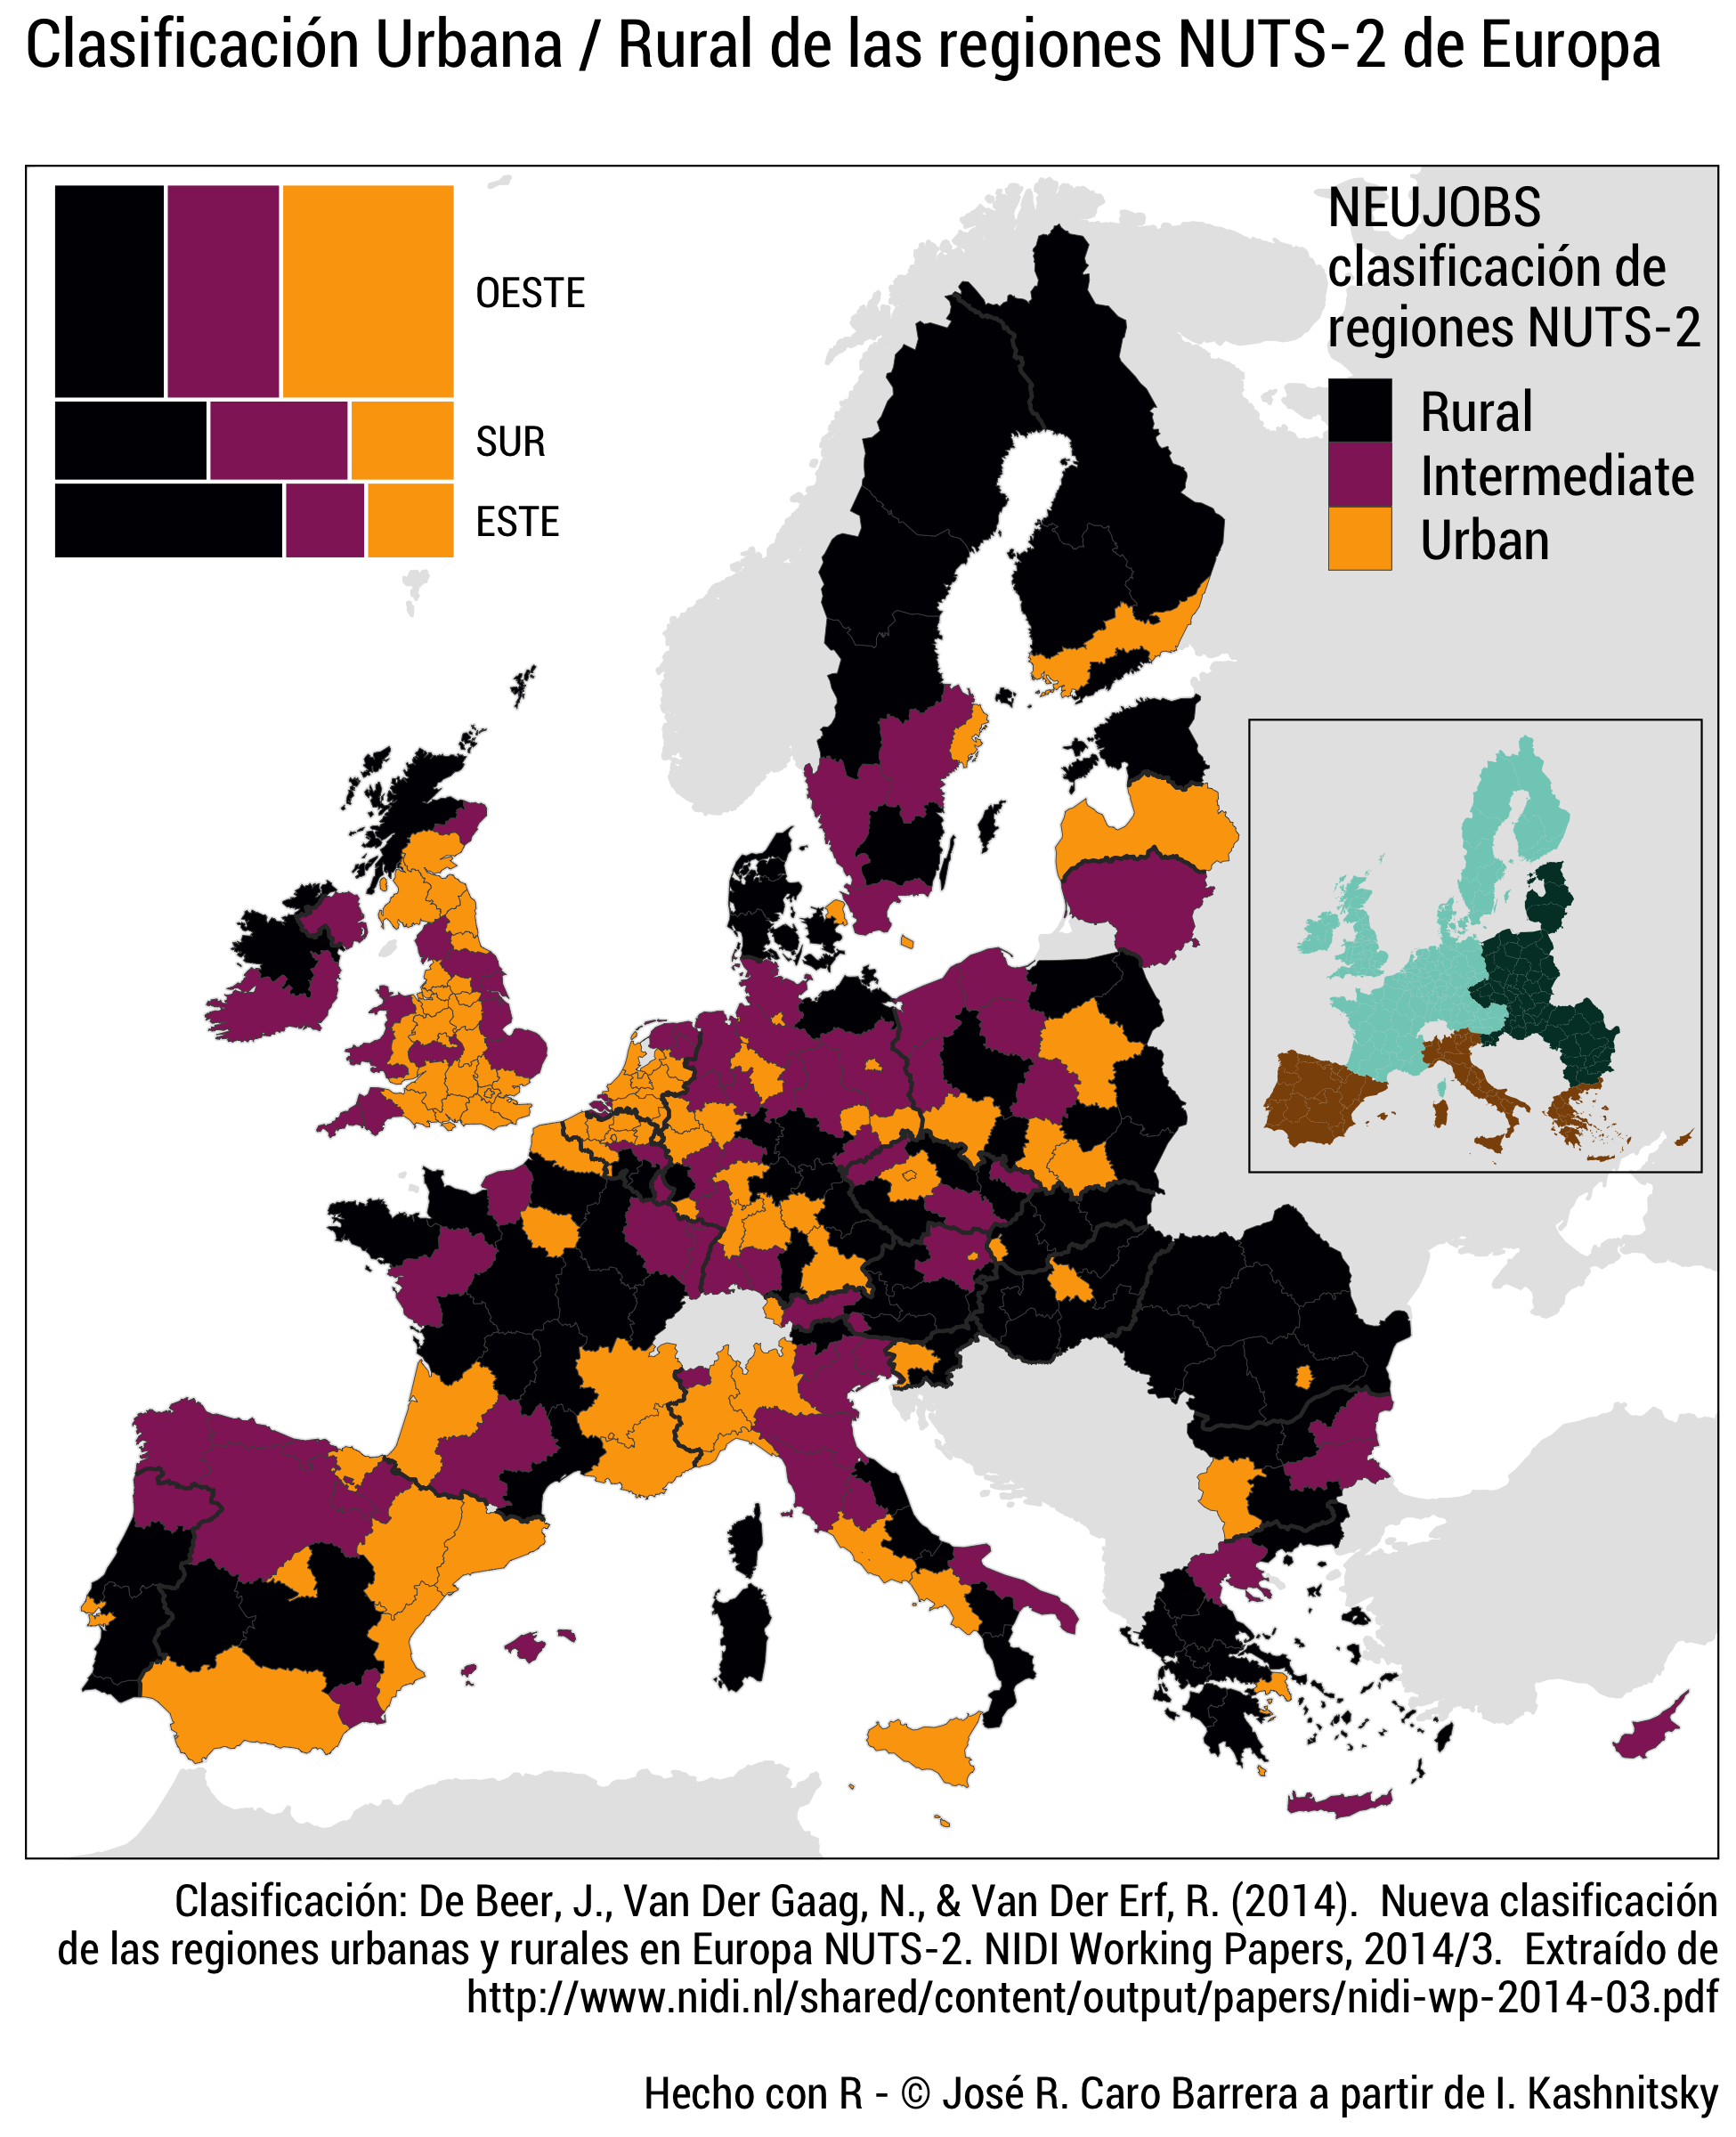
\includegraphics[scale=0.15]{Cap1/urban.png}
\vspace{-0.2cm}
\caption{Clasficaci\'on urbana/rural de las regiones NUTS-2 de Europa}\\ 
\textit{(Fuente: Eurostat)}
\end{figure}

\begin{figure}[!ht]
\centering
\hspace*{-0.6cm}\fbox{
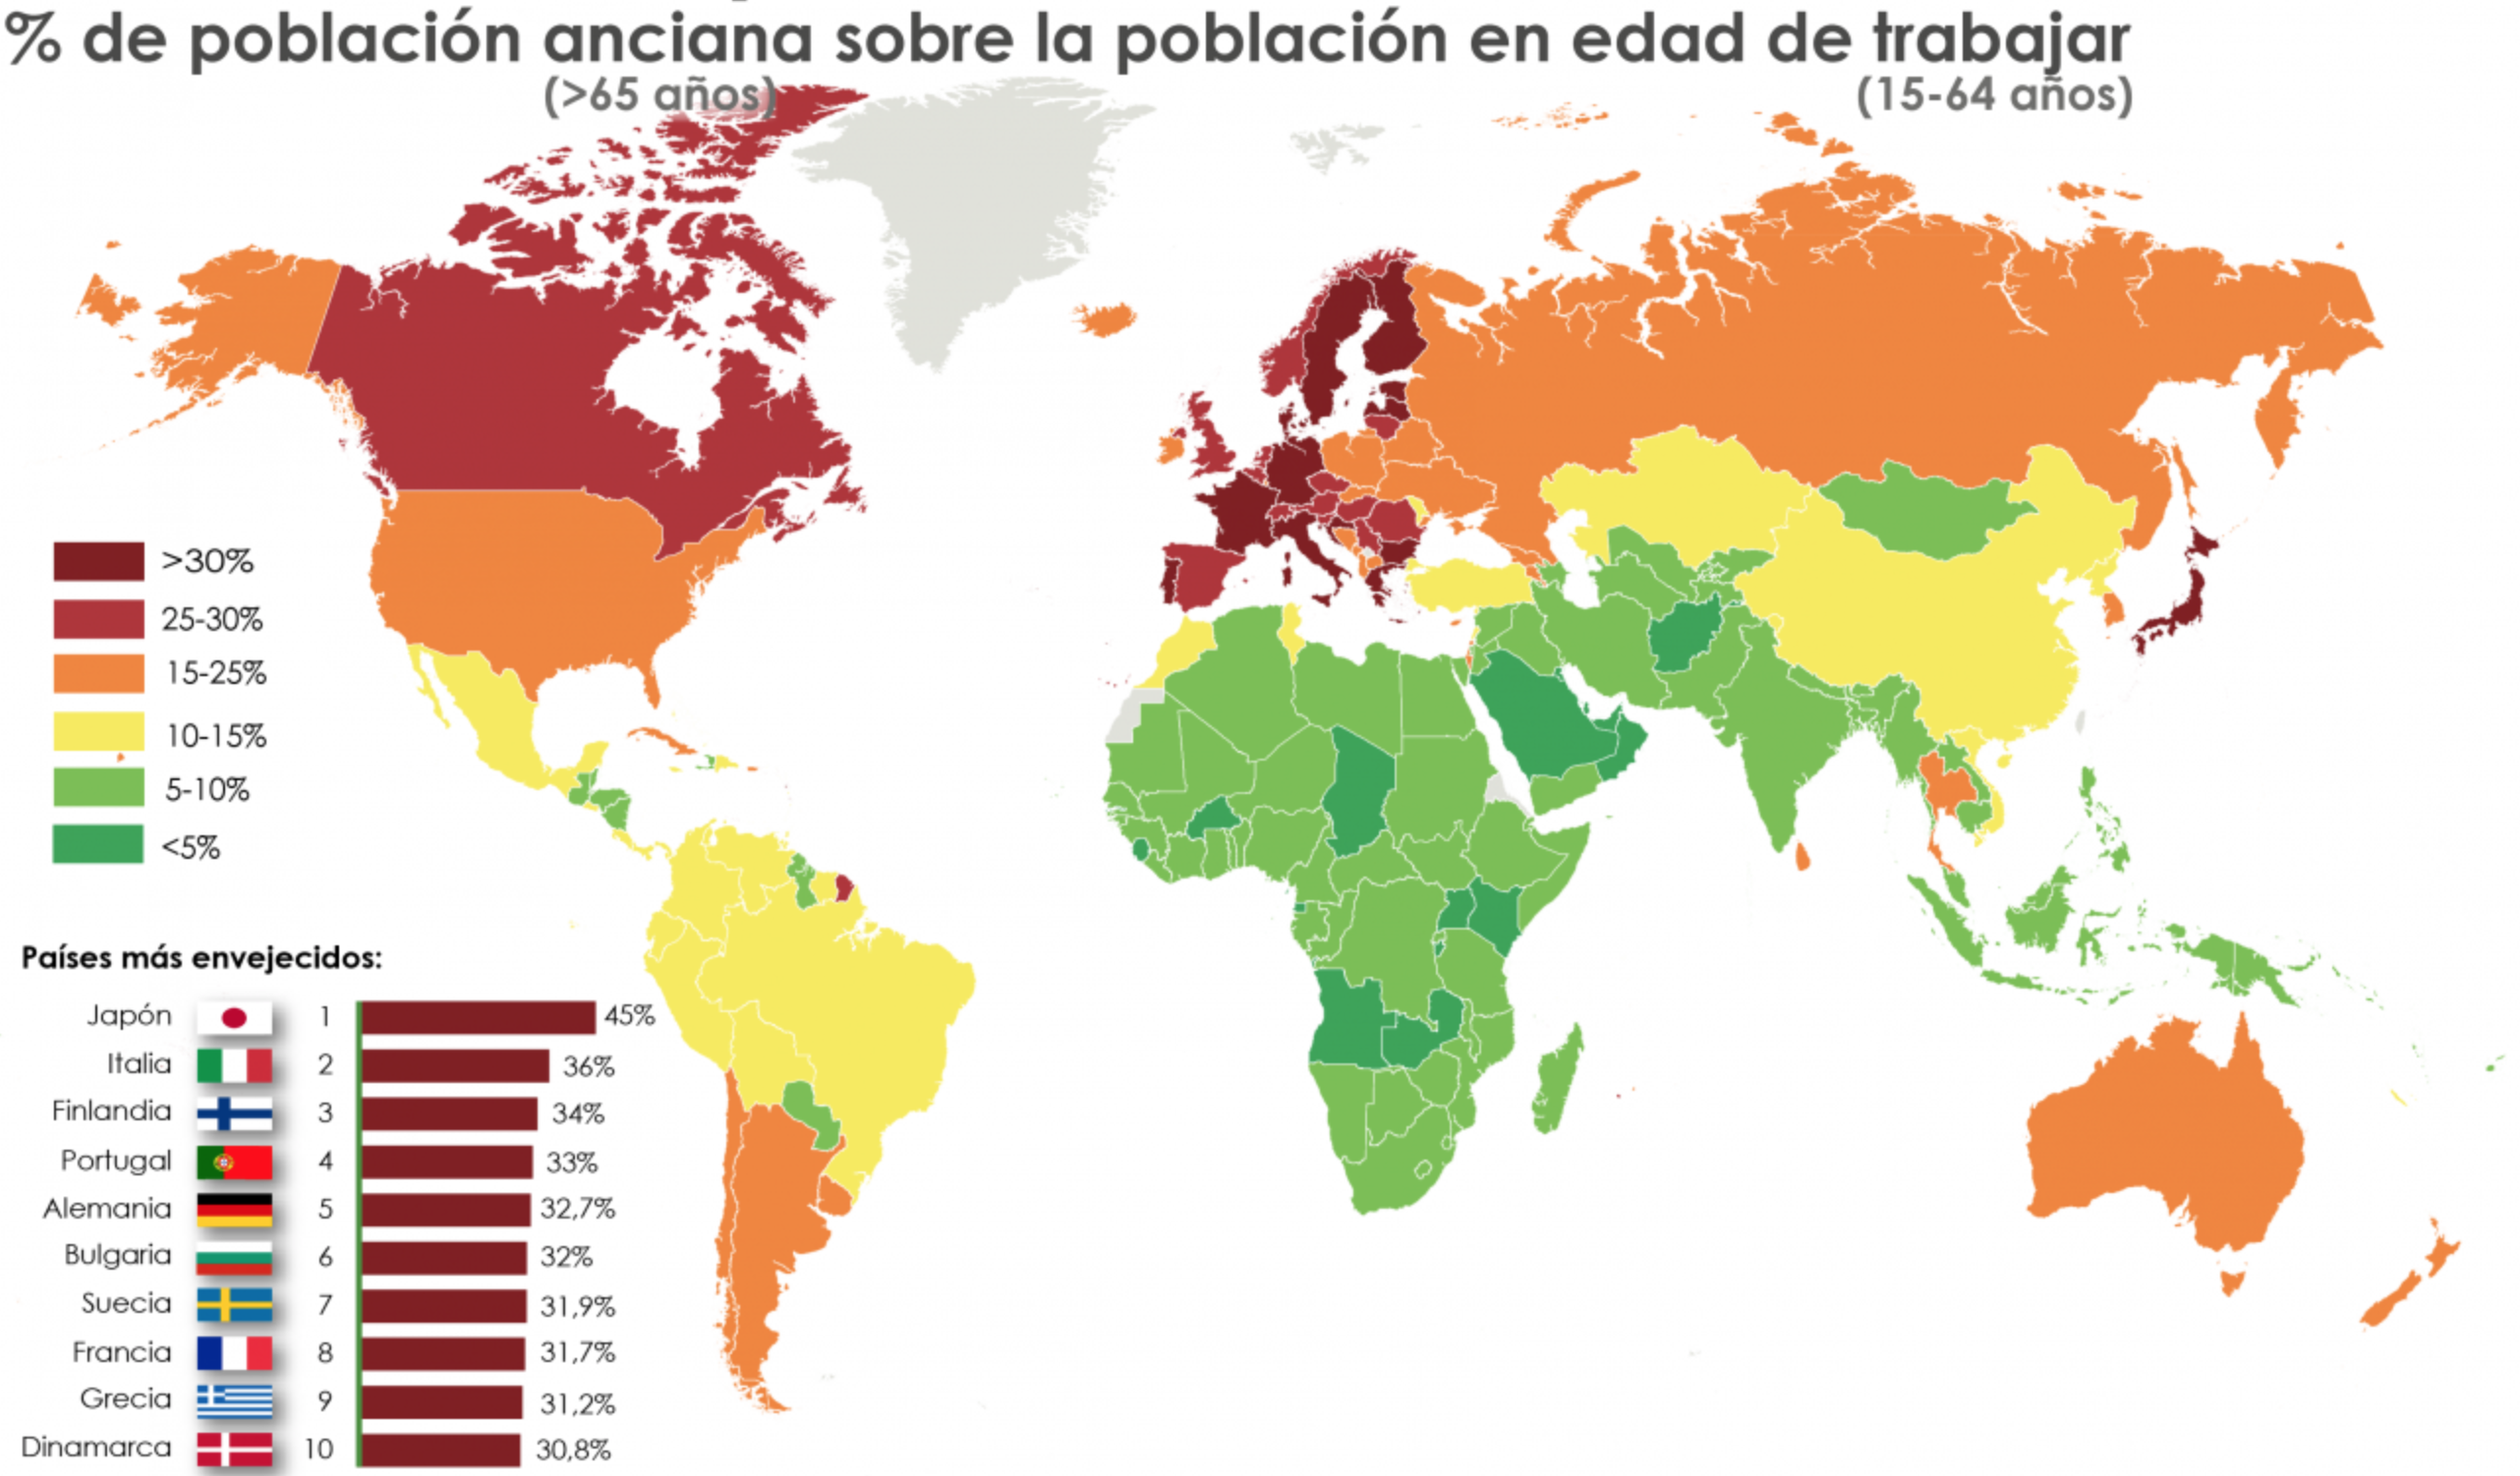
\includegraphics[scale=0.4]{Cap1/pesoancianos.png}}
\caption{\% de población anciana sobre la población en edad de trabajar.}\\
\textit{(Fuente: Banco Mundial, 2017)}
\end{figure}

\begin{wrapfigure}[22]{r}{0.6\textwidth}
\centering
\hspace*{-1.3cm}
\vspace{-0.3cm}
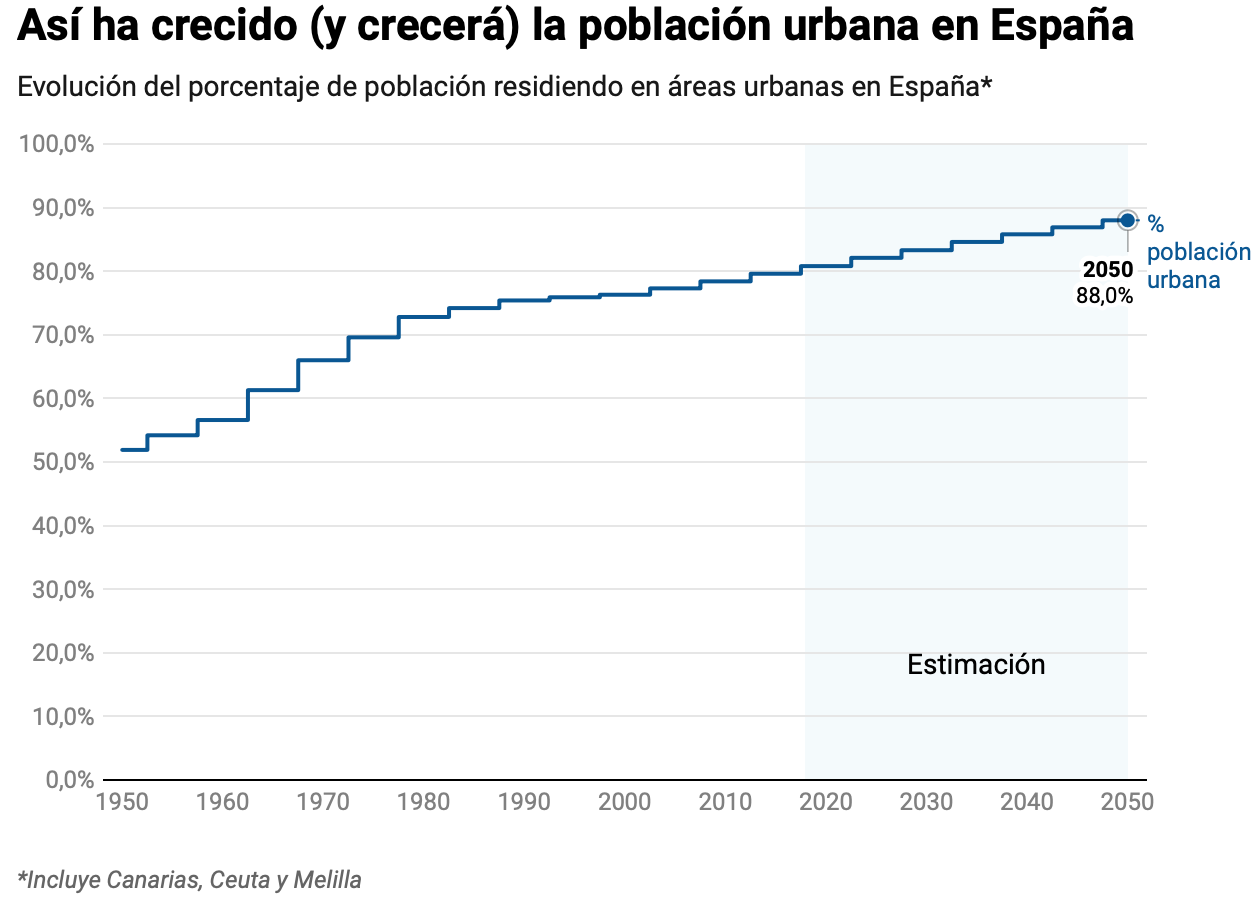
\includegraphics[width=0.7\textwidth]{Cap1/urbana.png}
%\vspace{-5pt}
\caption{Crecimiento y evolución de la población urbana en España}\\
\centering \textit{\small{Fuente: ONU}}
\end{wrapfigure}
España tampoco es ajena al proceso de despoblación rural y según la ONU, la brecha entre la población rural y urbana seguirá ensanchándose paulatinamente las próximas décadas en nuestro país. En 2018, el 80\% de la población española vivía en ciudades, según el Banco Mundial, y en 2050 será ya el 88\%, según las proyecciones de la \textit{División de Población de las Naciones Unidas Naciones Unidas} (ONU) \textbf{(ver figura 1.5)}. Antes, en 2035, la previsión es que casi un tercio, el 28\% de españoles, viva repartido entre Madrid y Barcelona. Será un 33\% si se le suman las tres siguientes urbes más grandes, Valencia, Sevilla y Zaragoza, contando las coronas metropolitanas\footnote{\texttt{https://www.eldiario.es/sociedad/Espana-vaciada-poblacion-Madrid-Barcelona\_0\_871763660.html}}.\\
\indent España tendrá en 2033 más de 49 millones de habitantes, 2.4 millones más que en 2019, según el INE, si se mantienen las tendencias de fecundidad, mortalidad y migraciones. En el censo actual (46,6 millones) las áreas metropolitanas de Madrid y Barcelona suman casi 11 millones (menos de un cuarto de la población española).

\newpage

\begin{figure}[H]
\centering
\hspace*{-1cm}
\fbox{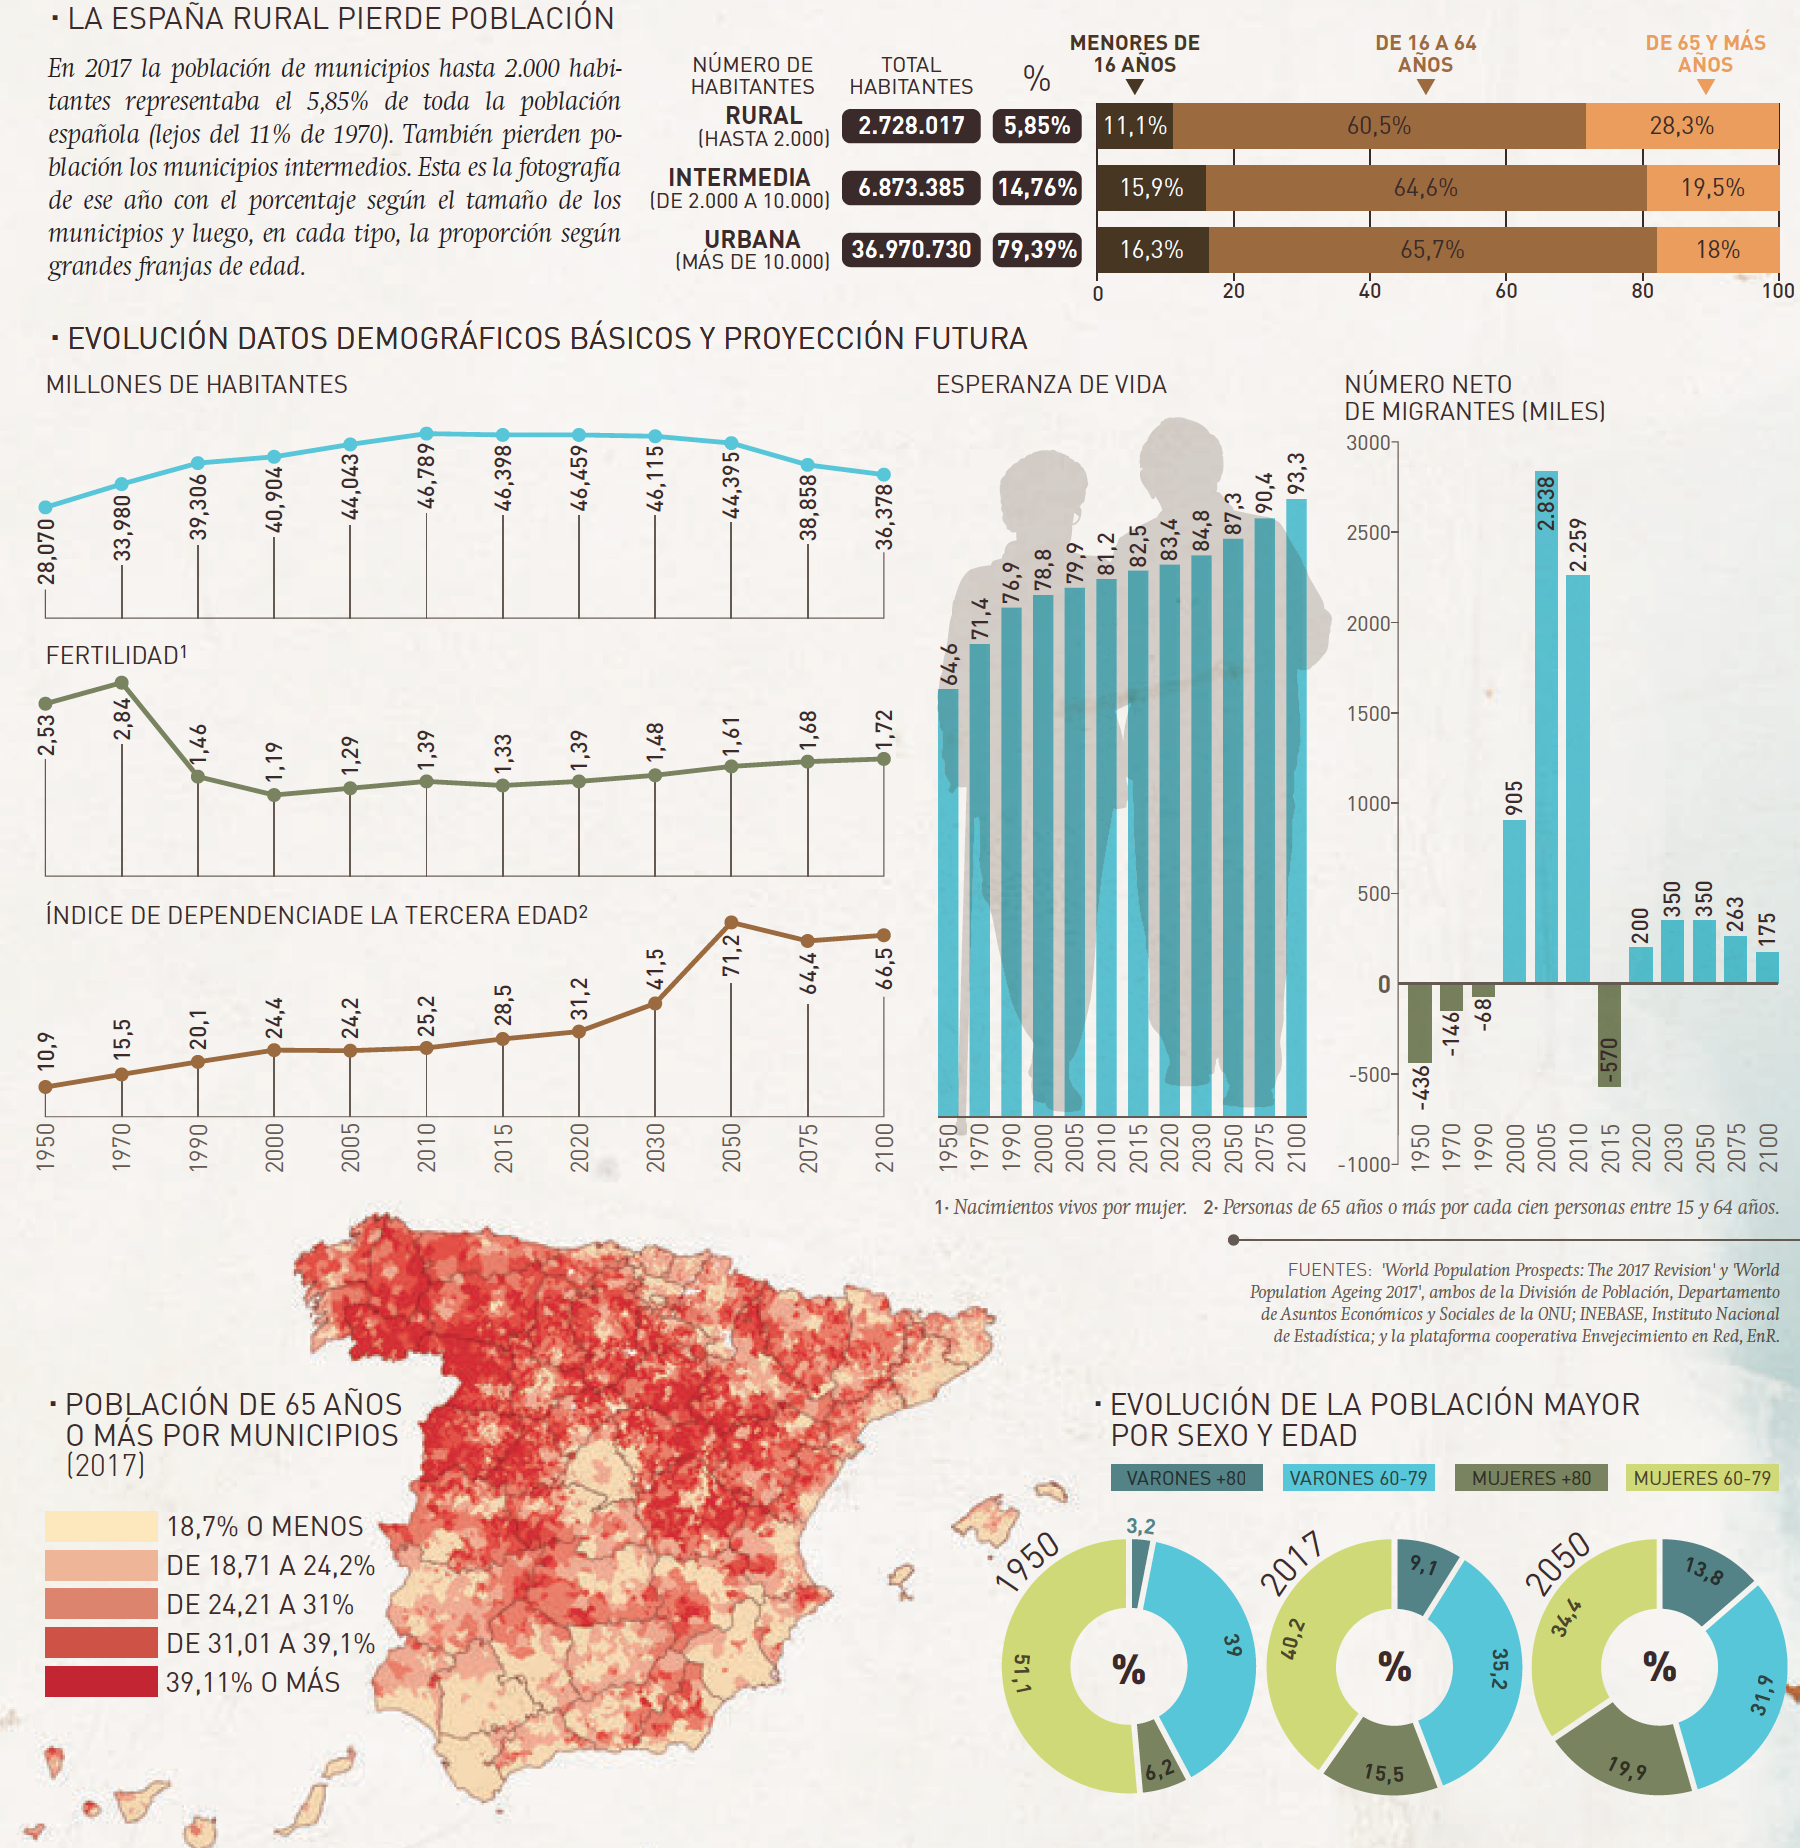
\includegraphics[scale=0.58]{Cap1/mayores1.png}}
\caption{Estructuras de poblaci\'on regional}\\
\textit{(Fuente: Eurostat)}
\end{figure}

En la \textbf{figura 1.7} se puede observar esa pérdida de población rural que comentábamos antes; además, no deja de ser esclarecedor el dato de proyección del índice de dependencia, el cual se situará en el 71,2\% en el año 2050. Esta tasa de dependencia es definida como la
ratio entre la poblaci\'on mayor de 65 años y la población de 15-64 años (González Martínez y Conde-Ruíz, 2018)\footnote{Si se calcula la tasa de dependencia como cociente entre la población mayor de 67 años y la población de 16-66 años, esta ratio pasará del 24,8\% actual al 60,2\% en 2050 con los datos de las proyecciones del INE (2018).}\textcolor{red}{[9]} y en comparación con el resto de países europeos, España será \textit{el país que experimentará el mayor aumento en tasa de dependencia}.

\newpage
%%%%%%%%%%%%%%%%%%%%%  SUBSECCION 1.2.1.: ESTRUCTURA DEMOGR\'AFICA %%%%%%%%%%%%%%%%

\subsection{La estructura demogr\'afica}

La estructura demogr\'afica es el modo en que est\'a repartida una poblaci\'on seg\'un cualquier clasificaci\'on de las personas que la componen (estado civil, nivel de estudios, regi\'on de residencia, edad o cualquier otro par\'ametro medible y clasificable).

\tikzset{every picture/.style={line width=0.75pt}} %set default line width to 0.75pt        
\begin{center}
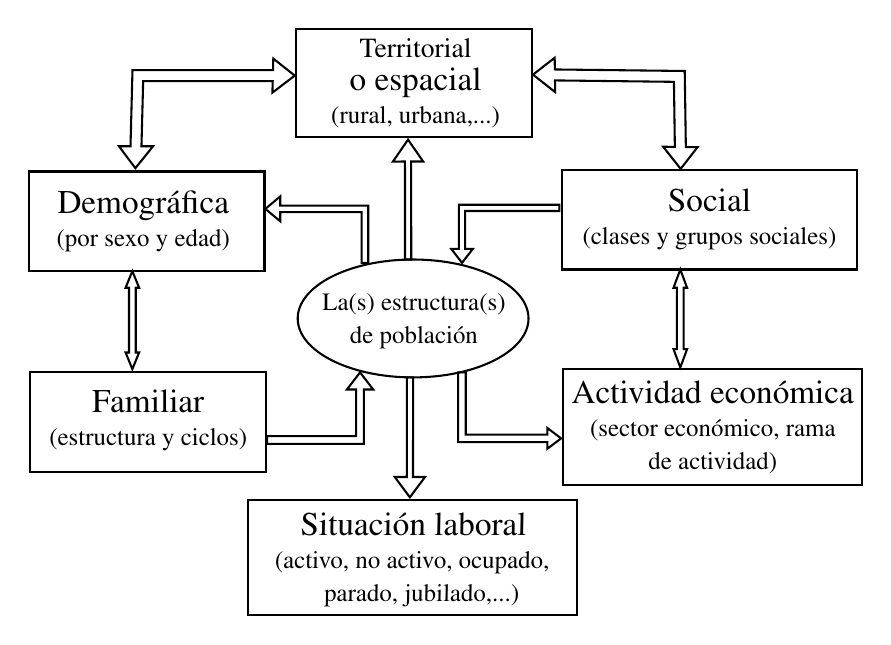
\begin{tikzpicture}[x=0.75pt,y=0.75pt,yscale=-1,xscale=1, scale=0.8]
%uncomment if require: \path (0,517); %set diagram left start at 0, and has height of 517
%Shape: Rectangle Top
\draw   (279,55) -- (421,55) -- (421,120) -- (279,120) -- cycle ;
%Shape: Rectangle First left
\draw   (118,141) -- (260,141) -- (260,201) -- (118,201) -- cycle ;
%Shape: Rectangle First right
\draw   (439,140) -- (617,140) -- (617,200) -- (439,200) -- cycle ;
%\draw   (439,140) -- (581,140) -- (581,200) -- (439,200) -- cycle ;
%Shape: Rectangle Bottom
\draw   (250,339) -- (448,339) -- (448,408) -- (250,408) -- cycle ;
%\draw   (277,339) -- (424.5,339) -- (424.5,399) -- (277,399) -- cycle ;
%Shape: Rectangle Second left
\draw   (119,262) -- (261,262) -- (261,322) -- (119,322) -- cycle ;
%Shape: Rectangle Second right
\draw   (440,260) -- (620,260) -- (620,330) -- (440,330) -- cycle ;
%\draw   (440,260) -- (588.5,260) -- (588.5,320) -- (440,320) -- cycle ;
%Shape: Ellipse
\draw   (280,229.5) .. controls (280,209.89) and (311.12,194) .. (349.5,194) .. controls (387.88,194) and (419,209.89) .. (419,229.5) .. controls (419,249.11) and (387.88,265) .. (349.5,265) .. controls (311.12,265) and (280,249.11) .. (280,229.5) -- cycle ;
%Left Up Arrow
\draw   (278.23,83.25) -- (264.76,93.5) -- (264.95,86.55) -- (186.93,86.55) -- (185.9,125.8) -- (192.85,125.8) -- (182.25,139) -- (172.34,125.8) -- (179.3,125.8) -- (180.5,79.95) -- (265.12,79.95) -- (265.3,73) -- cycle ;
%Left Up Arrow
\draw   (510.64,139.41) -- (500.1,126.08) -- (507.14,126.16) -- (506.58,86.99) -- (434.96,86.14) -- (435.06,93.18) -- (421.7,82.68) -- (434.76,72.49) -- (434.86,79.54) -- (513.09,80.46) -- (513.75,126.24) -- (520.79,126.32) -- cycle ;
%Up Down Arrow
\draw   (176.34,211) -- (180.42,201) -- (184.5,211) -- (182.46,211) -- (182.46,250) -- (184.5,250) -- (180.42,260) -- (176.34,250) -- (178.38,250) -- (178.38,211) -- cycle ;
%Up Arrow
\draw   (337.35,135) -- (346.45,121.8) -- (355.57,134.99) -- (348.33,134.99) -- (348.37,194) -- (344.63,194) -- (344.59,134.99) -- cycle ;
%Up Arrow
\draw   (356.67,325) -- (347.55,337.2) -- (338.45,324.97) -- (345.69,324.98) -- (345.77,265) -- (349.5,265) -- (349.43,324.99) -- cycle ;
%Bend Up Arrow
\draw   (318.5,196) -- (318.5,165.5) -- (269.5,165.5) -- (269.5,171) -- (260.5,163.5) -- (269.5,156) -- (269.5,161.5) -- (322.5,161.5) -- (322.5,196) -- cycle ;
%Bend Up Arrow
\draw   (381.22,262) -- (381.22,299.42) -- (430.33,299.42) -- (430.33,295.44) -- (438.62,301.72) -- (430.33,308) -- (430.33,304.02) -- (376.62,304.02) -- (376.62,262) -- cycle ;
%Bend Up Arrow
\draw  [line width=0.75]  (261.54,300.33) -- (315.22,300.33) -- (315.22,272.28) -- (309.61,272.28) -- (317.55,262) -- (325.5,272.28) -- (319.89,272.28) -- (319.89,305) -- (261.54,305) -- cycle ;
%Up Down Arrow
\draw   (506.34,211) -- (510.42,200) -- (514.5,211) -- (512.46,211) -- (512.46,248) -- (514.5,248) -- (510.42,259) -- (506.34,248) -- (508.38,248) -- (508.38,211) -- cycle ;
%Bend Up Arrow
\draw  [line width=0.75]  (437.54,164.8) -- (380.87,164.8) -- (380.87,187.63) -- (385.43,187.63) -- (378.97,196) -- (372.5,187.63) -- (377.07,187.63) -- (377.07,161) -- (437.54,161) -- cycle ;
% Text Node
\draw (351,88) node  [align=center] {{\fontfamily{ptm}\selectfont {Territorial }}\\{\large {\fontfamily{ptm}\selectfont  o espacial} }\\{\small {\fontfamily{ptm}\selectfont (rural, urbana,...)}}};
% Text Node
\draw (350,231) node  [align=center] {{\fontfamily{ptm}\selectfont {\small La(s) estructura(s)}}\\{\fontfamily{ptm}\selectfont {\small de poblaci\'on}}};
%\draw (339,231) node  [align=left] {{\fontfamily{ptm}\selectfont {\small  \ \ \ \ \ La(s) estructura(s)}}\\{\fontfamily{ptm}\selectfont {\small  \ \ \ \ \ \ \ \ \ de poblaci\'on}}};
% Text Node
\draw (187,171) node [align=center] {{\large {\fontfamily{ptm}\selectfont Demogr\'afica} }\\{\small {\fontfamily{ptm}\selectfont (por sexo y edad)}}};
% Text Node
\draw (190,291) node [align=center] {{\large {\fontfamily{ptm}\selectfont Familiar} }\\{\small {\fontfamily{ptm}\selectfont (estructura y ciclos)}}};
% Text Node
\draw (528,170) node [align=center] {{\large {\fontfamily{ptm}\selectfont Social} }\\{\small {\fontfamily{ptm}\selectfont (clases y grupos sociales)}}};
% Text Node
\draw (530,295) node  [align=center] {{\large {\fontfamily{ptm}\selectfont  Actividad econ\'omica} }\\{\small {\fontfamily{ptm}\selectfont (sector econ\'omico, rama}}\\{\small {\fontfamily{ptm}\selectfont  de actividad)}}};
%\draw (505,290) node  [align=left] {{\large {\fontfamily{ptm}\selectfont  \ \ \ Actividad econ\'omica} }\\{\small {\fontfamily{ptm}\selectfont  \ \ \ \ \ \ \ (sector econ\'omico, rama}}\\{\small {\fontfamily{ptm}\selectfont  \ \ \ \ \ \ \ \ \ \ \ \ \ \ \ \ de actividad)}}};
% Text Node
\draw (349,375) node [xslant=0.02] [align=left] {{\large {\fontfamily{ptm}\selectfont  \ \ \ Situaci\'on laboral} }\\{\small {\fontfamily{ptm}\selectfont  (activo, no activo, ocupado,}}\\{\small {\fontfamily{ptm}\selectfont  \ \ \ \ \ \ \ \ parado, jubilado,...)}}};

\end{tikzpicture}
\end{center}

Dicha estructura demogr\'afica va, indisolublemente unida a la variable \textit{tiempo}, de hecho, y seg\'un se\~nalan Vinuesa y otros (1997) \textcolor{red}{[10]}, \'esta desempe\~na un papel fundamental, pudiendo tener tres clasificaciones seg\'un el tipo de an\'alisis que se haga. De este modo, \textit{a)} si se refiere al momento en el que se hace la observaci\'on demogr\'afica se habla de tiempo \textbf{cronol\'ogico o de calendario}; \textit{b)}, si se trata del tiempo transcurrido desde la experimentaci\'on de un evento-origen, se trata de tiempo como \textbf{duraci\'on}; finalmente, \textit{c)} el tiempo como \textbf{l\'inea de vida}, se refiere a la cohorte de pertenencia de un individuo.\\

Dentro del an\'alisis demogr\'afico, el primer dato del que se ocupa esta disciplina es el de \textit{efectivo de una poblaci\'on}, distinguiendo entre \textit{poblaci\'on total} y \textit{poblaci\'on media}. Normalmente, la poblaci\'on presente en el momento de la observaci\'on se suele asociar a la \textit{poblaci\'on total}, aunque en los censos de poblaci\'on se suele diferenciar entre poblaci\'on `presente', es decir, con presencia f\'isica en el momento de la observaci\'on y poblaci\'on `de derecho', o sea, los residentes habituales en el lugar de la observaci\'on. A la poblaci\'on de un territorio durante un per\'iodo concreto, normalmente un a\~no, se le denomina \textit{poblaci\'on media}.\\

Por defecto, las clasificaciones m\'as simples de las poblaciones son seg\'un la edad y el sexo. Son las etapas iniciales y b\'asicas a la hora de definir a un individuo. La edad es una caracter\'istica que puede plantear ciertas dificultades dependiendo de si se trabaja con datos individuales o agrupados. En los datos agrupados, donde la edad y debido a que en un grupo referido a un a\~no de nacimiento habr\'ia individuos con diferente fecha, implicar\'ia hablar de \textit{generaci\'on}; es decir, en una muestra poblacional se puede establecer una clasificaci\'on de los individuos observados en base a la edad y a la generaci\'on a la que pertenece. Esta doble clasificaci\'on de los individuos se puede analizar mejor con el \textit{\textbf{diagrama de Lexis}}, procedimiento gr\'afico que permite clasificar los acontecimientos por per\'iodos anuales de observaci\'on, edad y generaci\'on de los individuos implicados. En la \textbf{figura 1.8}, se muestra este tipo de diagrama, donde sobre un eje de coordenadas  rectangulares se sit\'ua en la abscisa los a\~nos de calendario y en la ordenada, las edades.

\newpage
\begin{figure}[!ht]
\centering
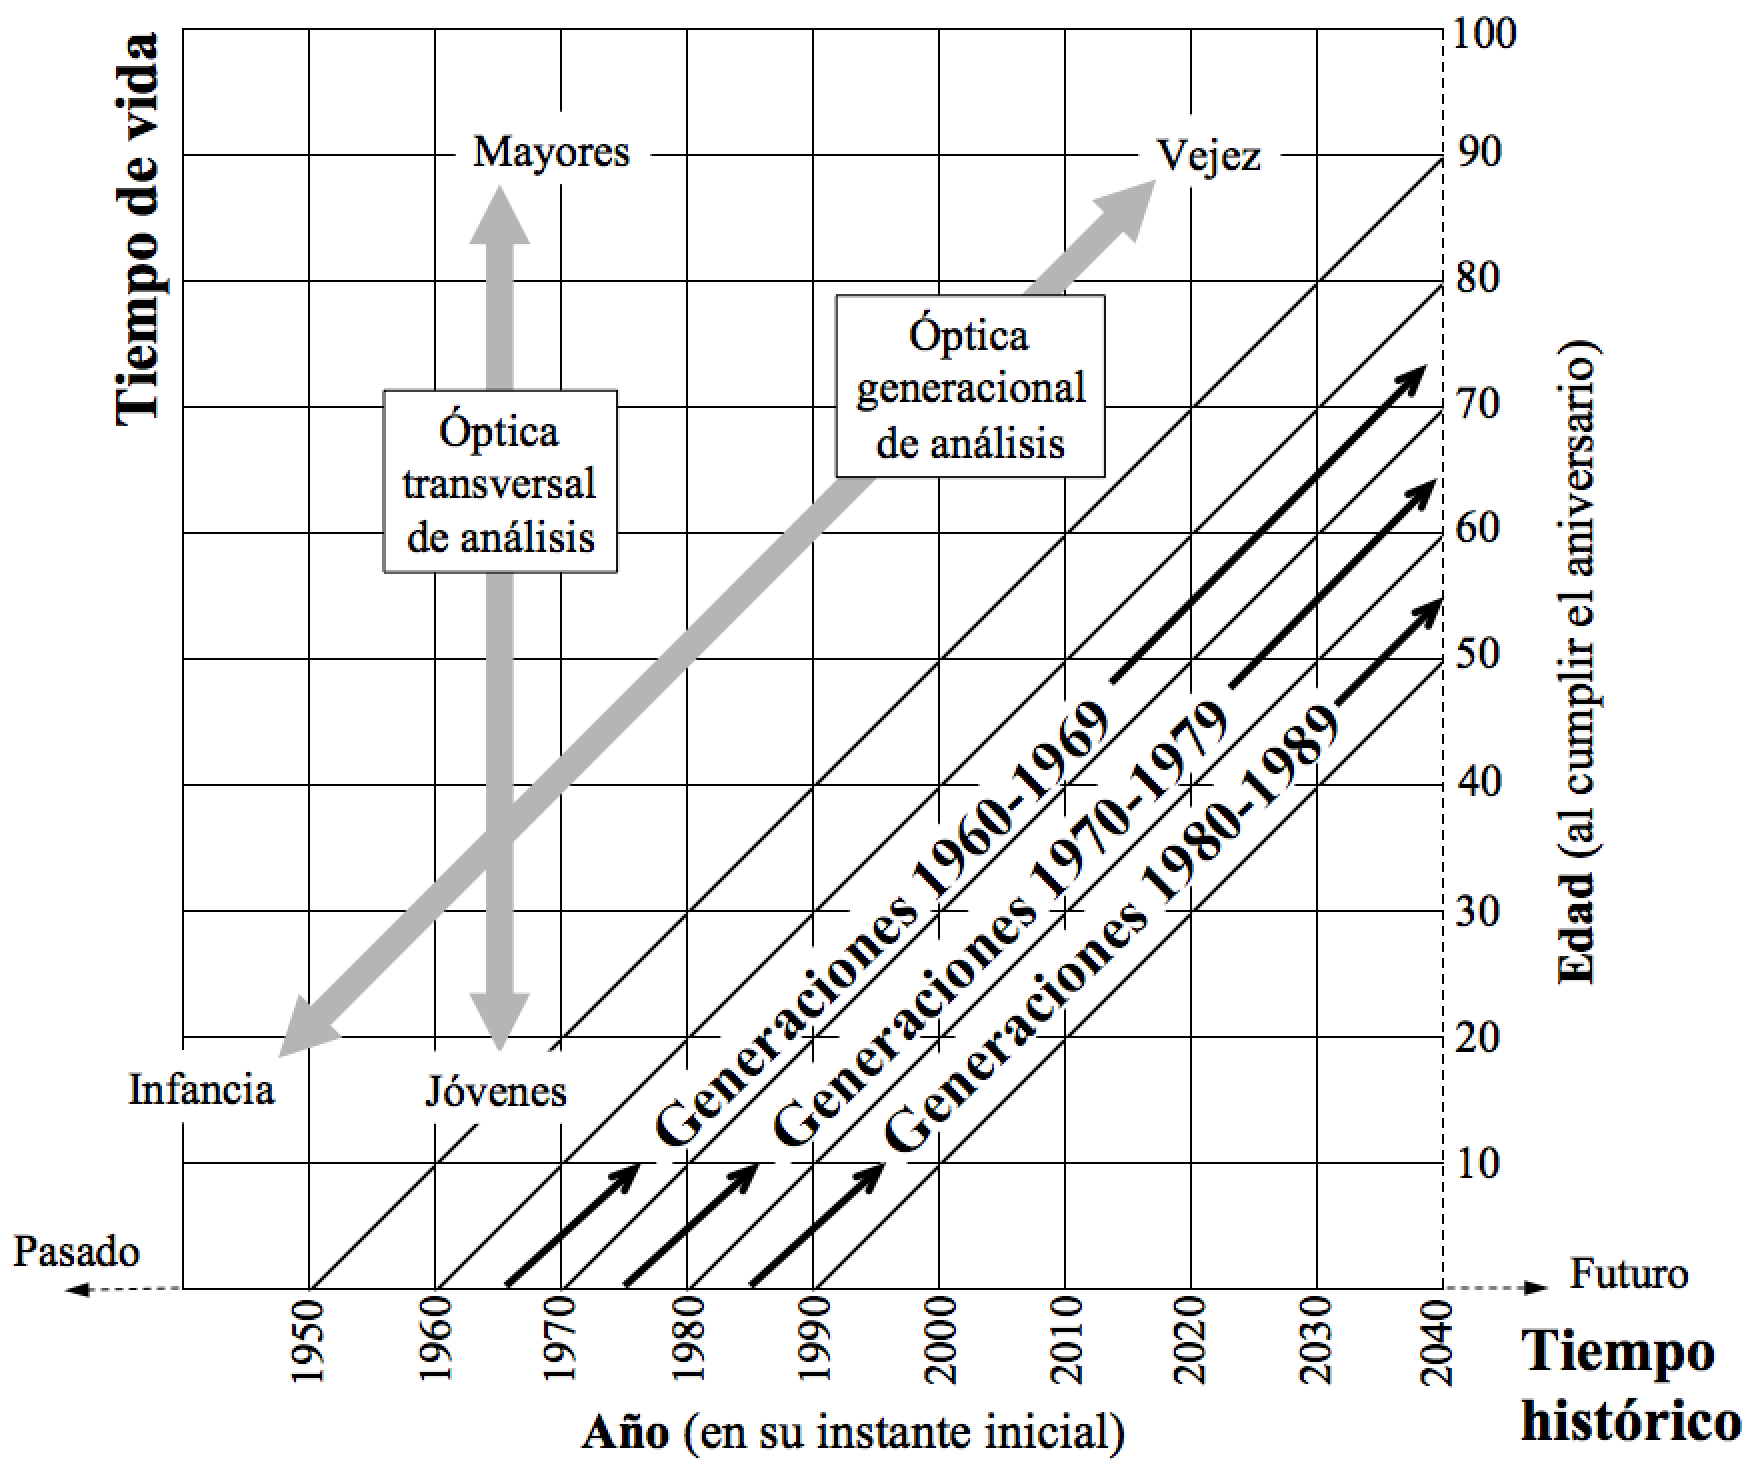
\includegraphics[scale=0.35]{Cap1/lexis.png}
\caption{Diagrama Lexis}\\
\textit{(Fuente: Elaboraci\'on propia)}
\end{figure}

Por ejemplo, en la \textbf{figura 1.9}, supongamos que el primer a\~no de calendario sea 1960, considerando un individuo nacido el 1 de enero de 1960. Se traza una OD, llamada l\'inea de vida, sobre la cual se inscriben los acontecimientos que la conciernen (matrimonio, nacimiento del primer hijo, del segundo,..., muerte). Esta l\'inea se traza de tal manera que, en todo momento, satisfaga la doble referencia de tiempo seg\'un la edad y de a\~no calendario. En esa misma figura, est\'an representadas las l\'ineas de vida de dos individuos, uno nacido el 1 de enero de 1960, casado a los 25 a\~nos y muerto a los 58 a\~nos; el otro, nacido el 1 de enero de 1973, casado a los 20 a\~nos , padre de un primer hijo a los 30 a\~nos, de un segundo a los 35 a\~nos y muerto a los 43 a\~nos.

%\newpage
\begin{figure}[!ht]
\centering
%\hspace*{-0.75cm}
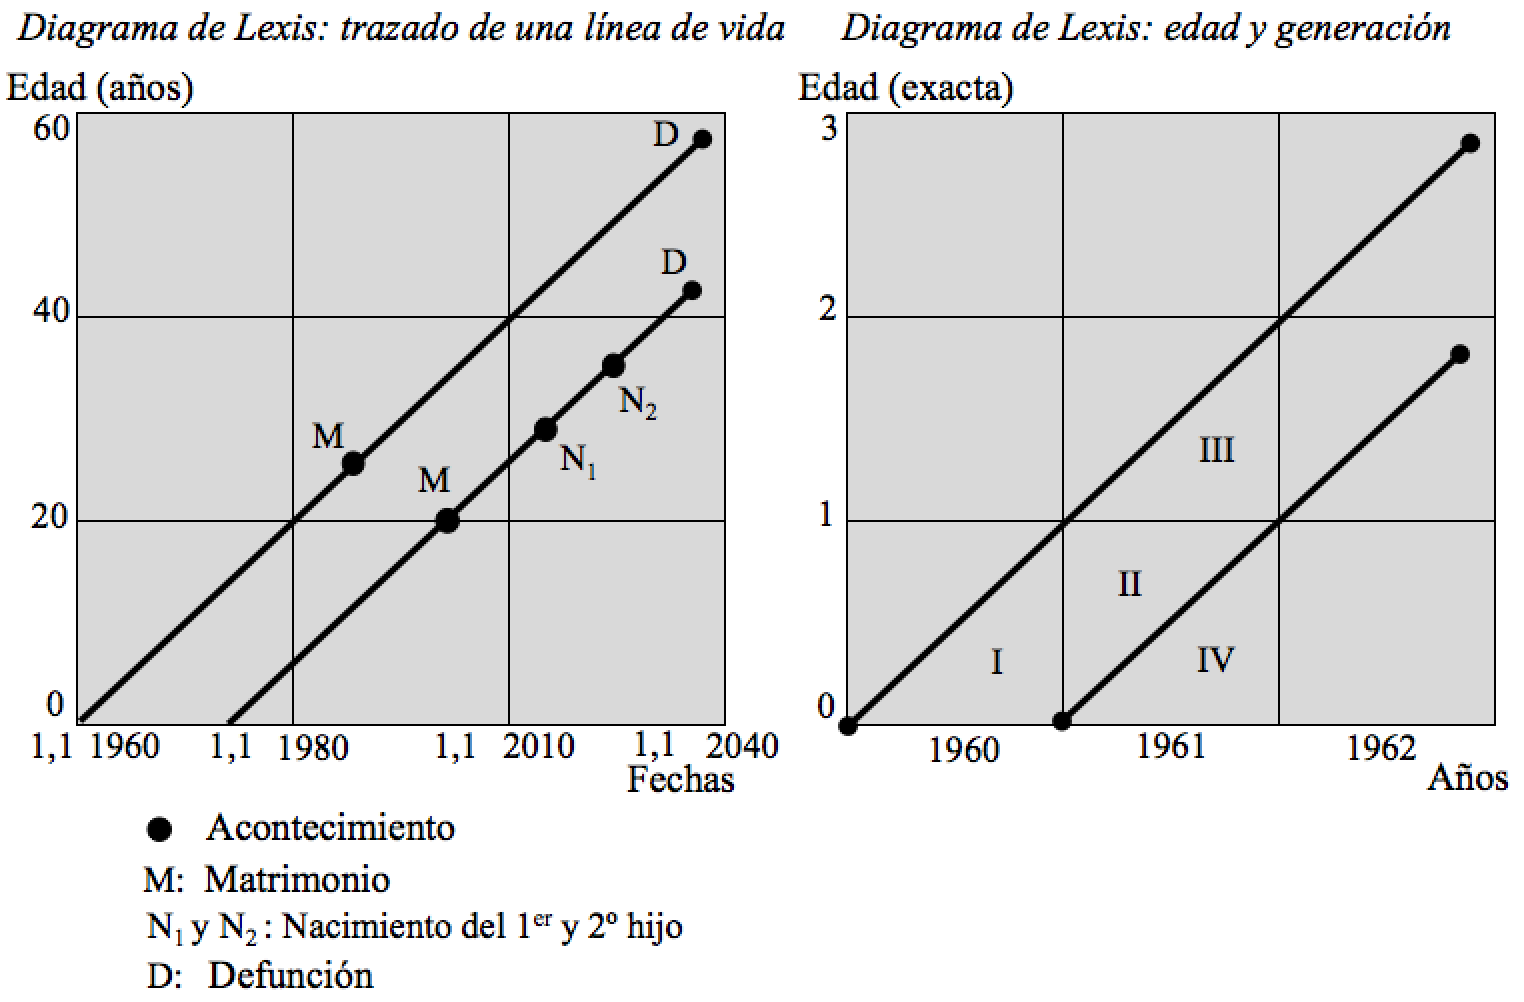
\includegraphics[scale=0.48]{Cap1/diagrlexis.png}
\caption{Modalidades de diagramas de Lexis}\\
\textit{(Fuente: Elaboraci\'on propia)}
\end{figure}

%\newpage
Las l\'ineas de vida de todos los individuos entre el 1 de enero de 1960 y el 31 de diciembre de 1960 pueden ser representadas por un conjunto de rectas paralelas a la primera bisectriz, pero de longitud desigual. Repitiendo la operaci\'on para todos los individuos nacidos en 1960, se obtiene la \textit{generaci\'on de 1960}. Se puede hacer lo mismo para 1961, 1962, etc. La representaci\'on de los datos sobre millares de individuos en un diagrama de Lexis consiste en indicar el n\'umero de l\'ineas vida que cortan los segmentos horizontales y verticales y el n\'umero de puntos-acontecimientos situados sobre una superficie dada.\\

\vspace{-0.3cm}

Los acontecimientos relativos a una misma edad se leen horizontalmente, los que conciernen al mismo a\~no civil, se leen verticalmente. De hecho, en el segundo diagrama de la \textbf{figura 1.9}, los acontecimientos que conciernen a la generaci\'on de 1960 durante un a\~no de calendario (1961, por ejemplo) se refieren a dos grupos de edades diferentes (II y III); los acontecimientos suceden a una edad cumplida (edad cero a\~nos cumplidos, por ejemplo), refiri\'endose a dos a\~nos calendario (I y II). Los acontecimientos relativos a un a\~no calendario y concernientes a los individuos que tienen la misma edad cumplida (por ejemplo, 0 a\~nos), se refieren a dos generaciones, en este caso 1960 y 1961 (II y IV).

\vspace{-0.3cm}

\subsubsection*{\textit{Distribuci\'on por sexo y edad.}}

Ya se ha mencionado anteriormente que tanto la edad como el sexo son las caracter\'isticas m\'as importantes en el an\'alisis demogr\'afico a la hora de definir una poblaci\'on.\\

\indent La \textbf{distribuci\'on por sexo} viene definida como el cociente a cada edad del efectivo masculino, \textit{Pm}, entre el efectivo femenino, \textit{Pf}, es decir \textit{Pm/Pf}, obteniendo as\'i la \textit{relaci\'on de masculinidad}. El mismo ratio pero a la inversa, esto es, \textit{Pf/Pm}, nos proporciona la \textit{relaci\'on de feminidad} (Tapinos, 1990) \textcolor{red}{[7]}.

Tal y como se puede ver en el \textbf{cuadro 1.2}, desde el nacimiento hasta los 54 a\~nos, la proporci\'on de los varones es superior a la de mujeres; a partir de los 54 a\~nos, el ratio de masculinidad se invierte, pasando a haber m\'as mujeres que hombres, en un ratio m\'as elevado. No obstante, en las edades superiores las diferencias son mayores a consecuencia de la mortalidad y la migraci\'on. Con todo ello, en la poblaci\'on total predomina ligeramente el sexo masculino, con un ratio \textit{Pf/Pm} de 1.02, seg\'un estimaciones de 2016 (\textbf{figura 1.10})\\

\vspace{-0.4cm}
\begin{table}[!htp]
 \begin{center}
 \hspace*{-0.3cm}\scalebox{0.75}{
   \begin{tabular}{ccccccc} \hline% <-- Alignments: 1st column left, 2nd middle and 3rd right, with vertical lines in between
\rowcolor{gray!30}\textbf{Al nacer} & \textbf{0-14 a\~nos} & \textbf{14-24 a\~nos} & \textbf{25-54 a\~nos} & \textbf{55-64 a\~nos} & \textbf{65 en adelante} & \textbf{Total poblaci\'on}\\ \hline 
   1.03 hombre/mujer & 1.07 hombre/mujer & 1.07 hombre/mujer & 1.02 hombre/mujer & 0.85 hombre/mujer & 0.81 hombre/mujer & 1.02 hombre/mujer \\ \hline 
\end{tabular}}\vspace{-0.2cm}
\caption{Ratio de sexo por intervalo de edad}\\
\textit{\small{(Fuente: Indexmundi.com)}}
   \label{tab:table1}
  \end{center}
\end{table}

\vspace{-0.8cm}
\noindent Por otro lado, como se muestra en la \textbf{figura 1.10} es interesante observar tambi\'en el ratio de sexo por pa\'is:\\

\vspace{-0.6cm}
\begin{figure}[!ht]
%\centering
\hspace*{-0.3cm}
\fbox{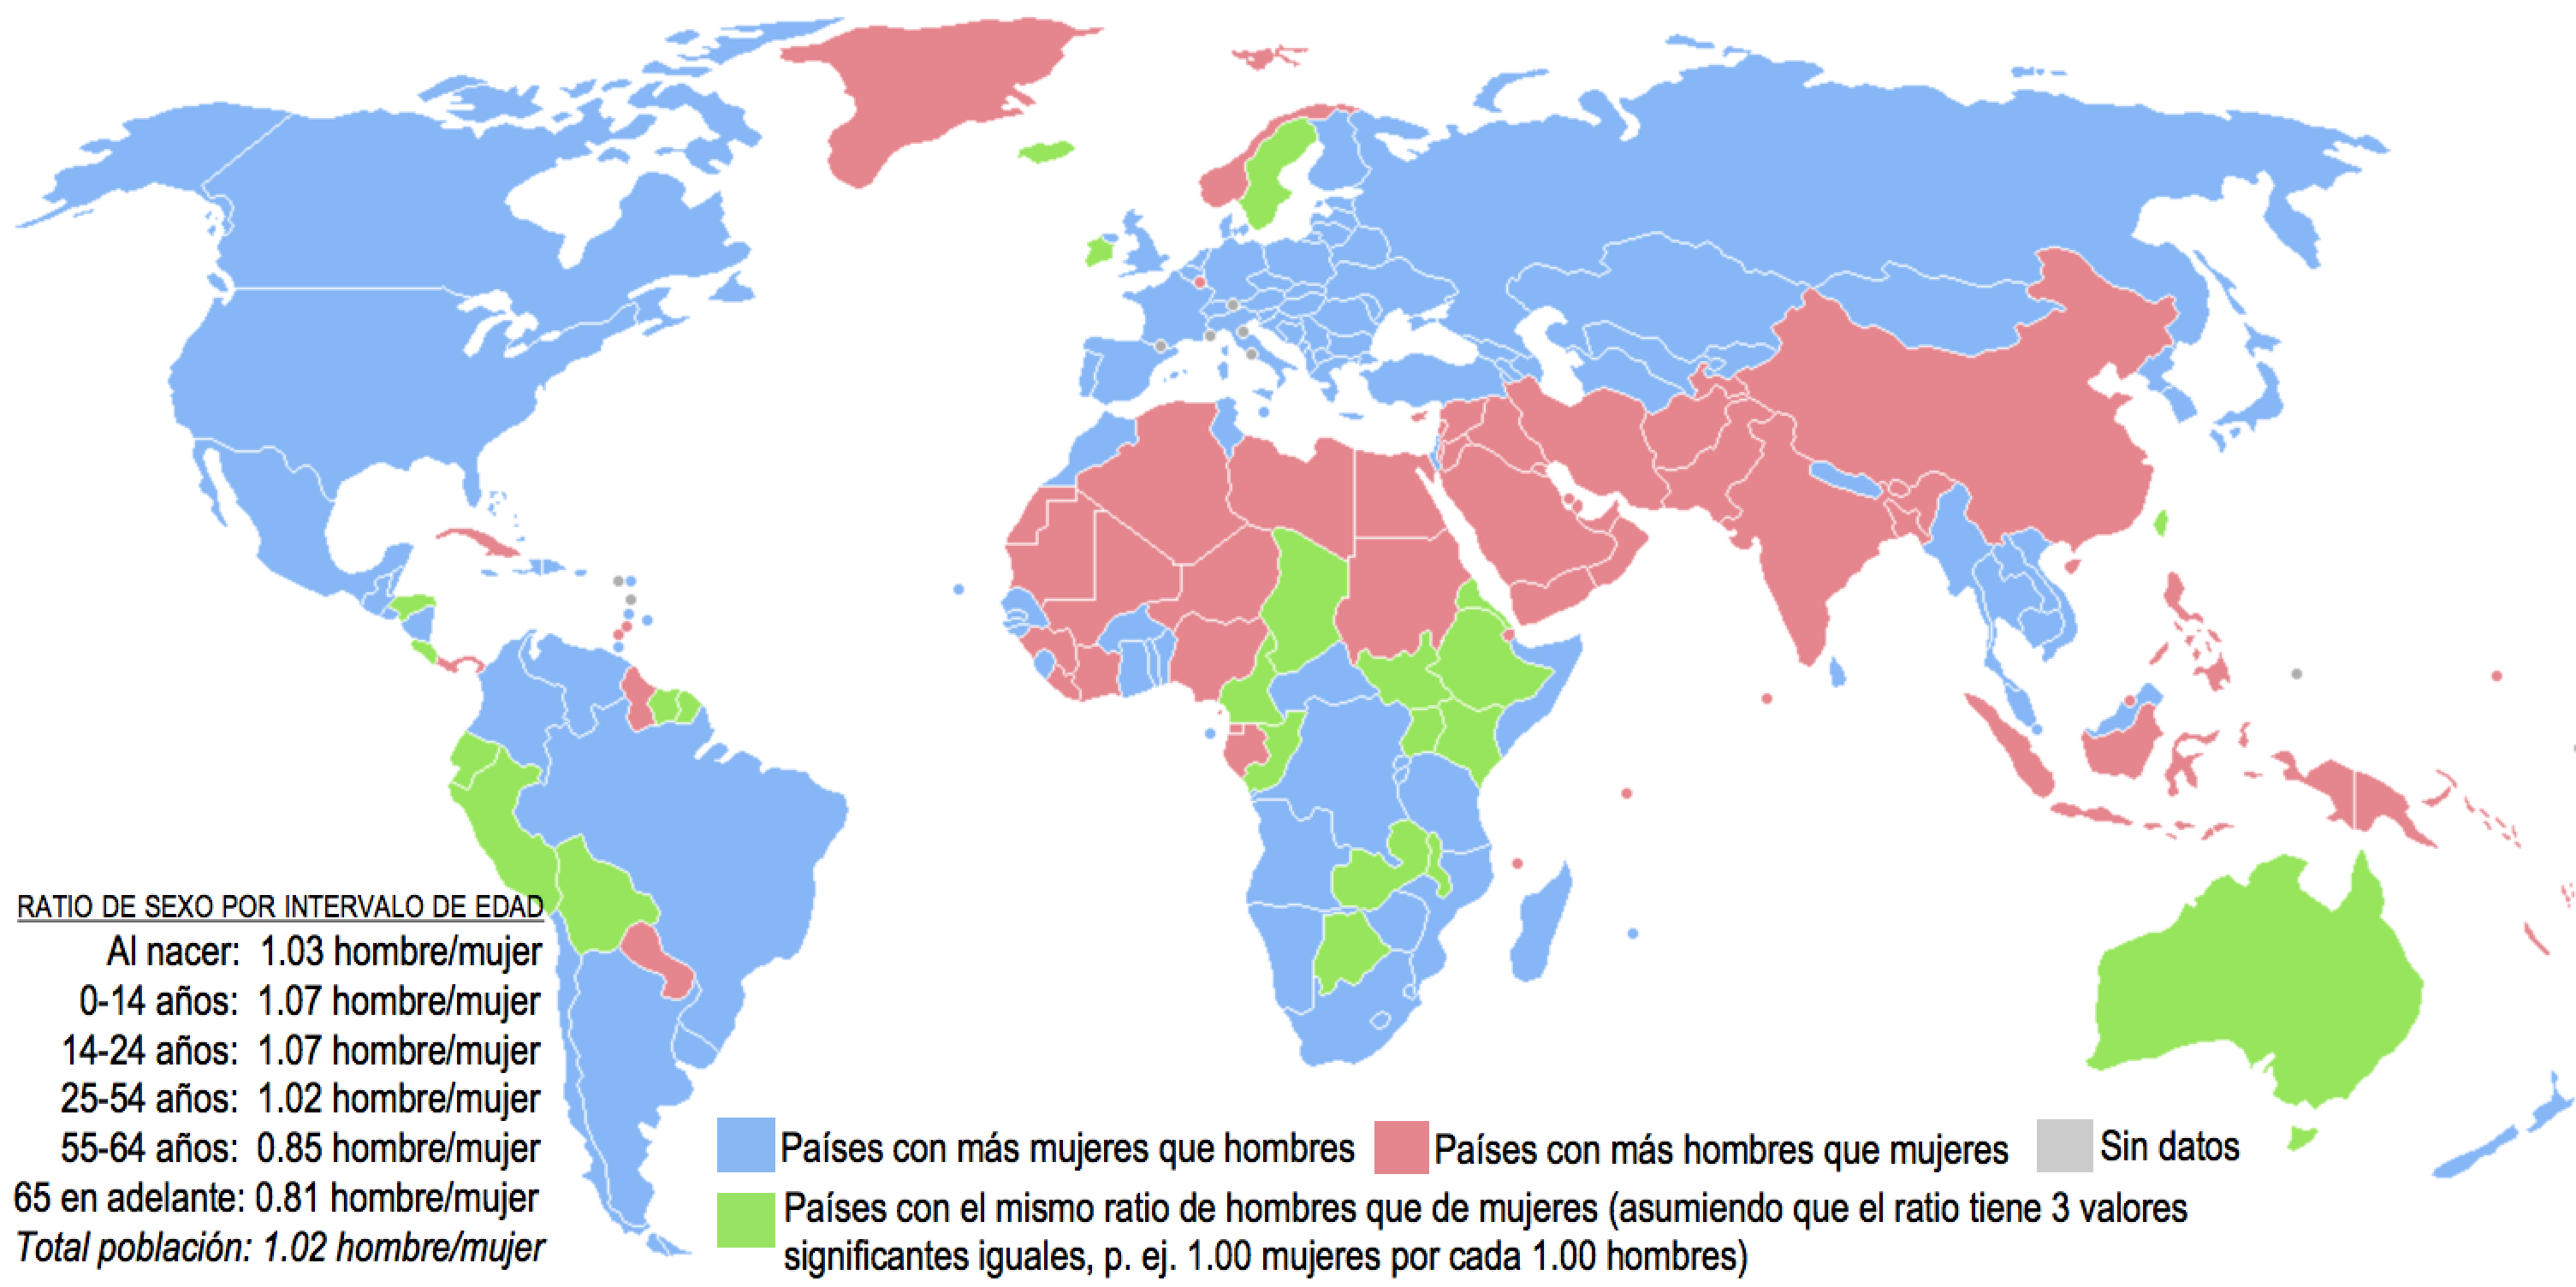
\includegraphics[scale=0.33]{Cap1/sexratio}}\vspace{-0.2cm}
\caption{Mapa del ratio de sexo por pa\'is y por intervalo de edad}
\centering\textit{\small{(Fuente: CIA World Factbook, 2016)}}
\end{figure}

\vspace{-0.4cm}
\noindent donde se puede apreciar que a pesar de haber un mayor n\'umero de pa\'ises con un ratio femenino m\'as alto (pr\'acticamente toda Europa, casi todo el contienente americano y algunos pa\'ises de \'Africa), en las zonas donde hay mayor n\'umero de hombres que de mujeres se encuentran pa\'ises como China, India, Nigeria, Indonesia y Pakist\'an, por ejemplo, que pertenecen a las regiones con m\'as poblaci\'on del mundo.\\

La \textbf{distribuci\'on por edad} permite clasificar poblaciones sobre la base del c\'alculo de \'indices, as\'i, los ratios m\'as comunes a la hora de clasificar a la poblaci\'on por edad son: \\
\indent-- La \textit{relaci\'on de dependencia}, viene dada por la proporci\'on de los individuos en edad de no generaci\'on de actividad econ\'omica -- clases de edad 0-19 a\~nos y m\'as de 65 a\~nos-- con respecto a los individuos en edad de actividad: 20 a 64 a\~nos. Estos dos \'indices desagregados no permite obtener, un \textit{\'indice de juventud} (inactivos j\'ovenes/poblaci\'on en edad activa) y un \textit{\'indice de vejez} (inactivos de edad avanzada/poblaci\'on en edad de actividad).\\

\vspace{-0.3cm}
-- La \textit{proporci\'on de activos} compara la poblaci\'on en edad activa con la poblaci\'on total. A veces, a esta proporci\'on se le llama \textit{tasa de actividad}, aunque realmente y siendo estrictos, la tasa de actividad es una media ponderada de la poblaci\'on en edad de actividad por las tasas de actividad por edades.\\

\vspace{-0.3cm}
-- El \textit{\'indice de reemplazo de la poblaci\'on en edad de actividad}, que relaciona las entradas en <<actividad>> con las <<salidas>> de actividad.

\subsubsection*{\textit{La pir\'amide de edades.}}

De todos los instrumentos de an\'alisis demogr\'afico conocidos, la \textit{pir\'amide de edades} (tambi\'en llamada \textit{pir\'amide de poblaci\'on}), es el m\'as \'util para explicar la distribuci\'on por edad y sexo de una poblaci\'on. B\'asicamente se trata de construir dos histogramas de barras (o un histograma diferenciando dos cuadrantes: la izquierda para los hombres y la derecha para las mujeres, de ah\'i su utilidad para explicar el atributo del sexo) sobre un eje cartesiano donde el eje de abscisas representa las proporciones (o efectivos) y el eje de ordenadas las edades o grupos de edad. La confecci\'on de una pir\'amide de poblaci\'on no entra\~na grandes dificultades, a excepci\'on de algunos aspectos que hay que tener en cuenta a la hora de confeccionar los grupos de edad, por ejemplo, problema derivado de la desagregaci\'on de los datos, as\'i como la elecci\'on de la representaci\'on de las frecuencias (en cifras absolutas o convenientemente transformadas en valores relativos), lo cual depender\'a del uso que se le vaya a dar a tal instrumento.\\

Lo verdaderamente interesante o \'util de la pir\'amide de edad es su lectura e interpretaci\'on. Aparte de ofrecer una imagen global de la evoluci\'on din\'amica de una poblaci\'on, si se construye con cierta periodicidad, la forma de su silueta denota los cambios experimentados por la poblaci\'on debido a los fen\'omenos demogr\'aficos (natalidad, mortalidad y migraci\'on), ya que estos van modelando la composici\'on de la pir\'amide a lo largo del tiempo. En la \textbf{figura 1.11} se muestran las pir\'amides de poblaci\'on de diferentes pa\'ises, por ejemplo, \textbf{Yemen} presenta una \textbf{estructura joven}, con una forma c\'oncava y una base desarrollada, como consecuencia de una mortalidad por edades baja y de una fecundidad menor. \textbf{China}, por su parte, presenta una \textbf{poblaci\'on madura o en transici\'on} donde hay mayor igualdad entre las poblaciones joven y adulta y un porcentaje de poblaci\'on vieja m\'as reducido; los \textbf{Estados Unidos}, a pesar de tener una poblaci\'on tambi\'en madura, presenta la variante de la inmigraci\'on (tanto masculina como femenina) en la l\'inea m\'as cl\'asica de pa\'is tradicionalmente inmigratorio y rico (al igual que Canad\'a o Australia).\\ 

En cambio, pa\'ises como \textbf{Rusia y Jap\'on} est\'an caracterizados por una \textbf{estructura demogr\'afica madura o regresiva}, con una base progresivamente debilitada (a causa de una ca\'ida prolongada en el tiempo de la fecundidad, una c\'uspide desarrollada (consecuencia de una larga esperanza de vida de la poblaci\'on) y unos grupos de edades adultos importantes. Particularmente curioso es el caso de \textbf{Catar} y la mayor\'ia de los pa\'ises de Oriente Medio productores de petr\'oleo, donde a la estructura demogr\'afica propia, la cual suele ser joven, se suma una inmigraci\'on adulta joven masculina de car\'acter laboral, debido a la atracci\'on que ejercen estos pa\'ises por motivos de trabajo.\\

Por otro lado, la pirámide de edad pone de manifiesto la proporción de gente anciana, la cual no es la misma en cada población, ni tampoco lo es la tasa de envejecimiento de la misma; es más, edad cronológica y edad funcional pueden diferir, ya que por ejemplo, algunas personas pueden trabajar productivamente hasta la edad de 70 u 80 años, mientras que otras se vuelven improductivas a una edad más temprana; ello depende del tipo de trabajo que se desempeñe y el país. Además, la proporción de la población anciana crece conforme a los ingresos per cápita, lo cual es lógico pues la esperanza de vida es mayor en países más industrializados, como resultado de las condiciones sanitarias, asistenciales y de calidad de vida (World Bank, 1994) \textcolor{red}{[11]}.
%\newpage
\begin{figure}[H]
\centering
%\hspace*{-0.75cm}
\fbox{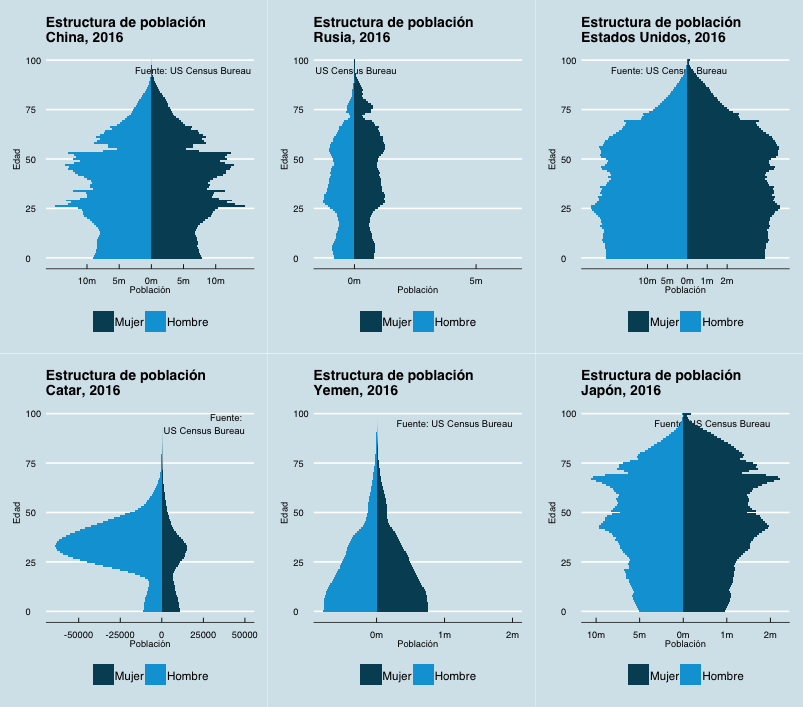
\includegraphics[scale=0.52]{Cap1/piramides.png}}
\caption{Comparativa de las pir\'amides de poblaci\'on de algunos pa\'ises}\\
\textit{(Fuente: Elaboraci\'on propia a partir de datos de U.S. Census Bureau)}
\end{figure}

Seg\'un lo anterior, y de acuerdo con \textcolor{red}{[10]}, en pa\'ises donde la evoluci\'on de su estructura viene determinada y desequilibrada por los flujos migratorios, la utilidad de las pir\'amides de edad para estudiar esta din\'amica y prever los efectos de la composici\'on en la poblaci\'on es de especial importancia.

%%%%%%%%%%%%%% SUBSECCION 1.2.2.: ANÁLISIS LONGITUDINAL Y TRANSVERSAL %%%%%%%%%%%%%%%%%%%%%%
\subsection{An\'alisis longitudinal y an\'alisis transversal}

A la hora de estudiar los cambios demogr\'aficos y sus mecanismos existen dos tipos de an\'alisis seg\'un el enfoque hacia el que se oriente. De este modo, el \textbf{\textit{an\'alisis longitudinal o hist\'orico}} es aquel en el que se fija un grupo de personas (ya sea una cohorte o una generaci\'on) y se sigue su evoluci\'on a trav\'es del tiempo, estudiando los diferentes fen\'omenos que le afectan.\\ 

Por el contrario, el \textbf{\textit{an\'alisis transversal}} es aquel que fija un periodo de tiempo, por ejemplo, una a\~no, y se siguen todos los acontecimientos ocurridos durante ese periodo de tiempo: nacimientos, matrimonios y muertes.\\

\vspace{-0.2cm}
El an\'alisis longitudinal plantea el inconveniente de que no puede ser calculado hasta despu\'es de la ocurrencia del fen\'omeno, presentando as\'i una visi\'on diacr\'onica (en el sentido de que analiza la evoluci\'on a trav\'es del tiempo)  de los fen\'omenos demogr\'aficos \textcolor{red}{[10]}, por ello, este an\'alisis no es muy frecuente. En cambio, el an\'alisis transversal es una aproximaci\'on en la que considera el momento de la observaci\'on. Es decir, tiene perfecta correspondencia temporal con el fen\'omeno que se observa.\\

\vspace{-0.2cm}
Como vimos en el punto 1.2.1, las relaciones entre ambos an\'alisis y el diagrama de Lexis vienen dadas seg\'un el enfoque u objetivo del estudio; as\'i, el an\'alisis longitudinal respecto a dicho diagrama se fundamenta en el estudio de una generaci\'on en el curso de varios a\~nos; por contra, el an\'alisis transversal respecto al diagrama de Lexis tiene como objetivo el estudio de las caracter\'isticas que tiene una poblaci\'on formada por varias cohortes en un periodo determinado.\\

\vspace{-0.2cm}
Estos an\'alisis nos sirven para entender a las poblaciones y son la base de herramientas muy \'utiles como las tablas de mortalidad (por ejemplo y entre otras), las cuales veremos m\'as adelante.
%\newpage
%%%%%%%%%%%%%%%%%% SECCION 1.3.: MUNDO PREPARADO PARA ENVEJECER %%%%%%%%%%%%%%%%

\section{?`Est\'a el mundo preparado para envejecer? (La ``vieja Europa'' est\'a ``vieja'')}

La arque\'ologa lituana Marija Gimbutas\footnote{\textit{``Diosas y dioses de la vieja Europa'' (1974).}}, cuyas investigaciones sobre el neol\'itico y la prehistoria se centraron en el sureste de Europa, en concreto, en la cultura pre-indoeuropea, fue la que acu\~n\'o el t\'ermino \textit{``vieja Europa''} para referirse a una cultura matrifocal y probablemente matrilineal, agr\'icola y sedentaria, igualitaria y pac\'ifica.\\ 
M\'as recientemente\footnote{\texttt{https://www.elcato.org/la-vieja-europa}}, durante la batalla diplom\'atica por ir a la guerra contra Irak, el secretario de defensa estadounidense, Donald Rumsfeld, introdujo el t\'ermino \textit{``vieja Europa''} para puntuar la oposici\'on de Alemania y Francia al uso de la fuerza en el inminente conflicto. Sea como fuere, el t\'opico de referirse al continente europeo como \textit{``la vieja Europa''} cuando se le compara con otros continentes, nunca ha sido m\'as cierto. En la \textbf{figura 1.12} se pueden observar los veinte pa\'ises con mayor esperanza de vida. De estos, trece son europeos (con Espa\~na en quinta posici\'on con una esperanza de vida de 82,8 a\~nos), seis asi\'aticos y uno perteneciente al continente americano. Por lo tanto, es un hecho constatado que la poblaci\'on europea es m\'as vieja. 
\vspace{-0.3cm}
\begin{figure}[H]
\centering
\hspace*{-0.75cm}
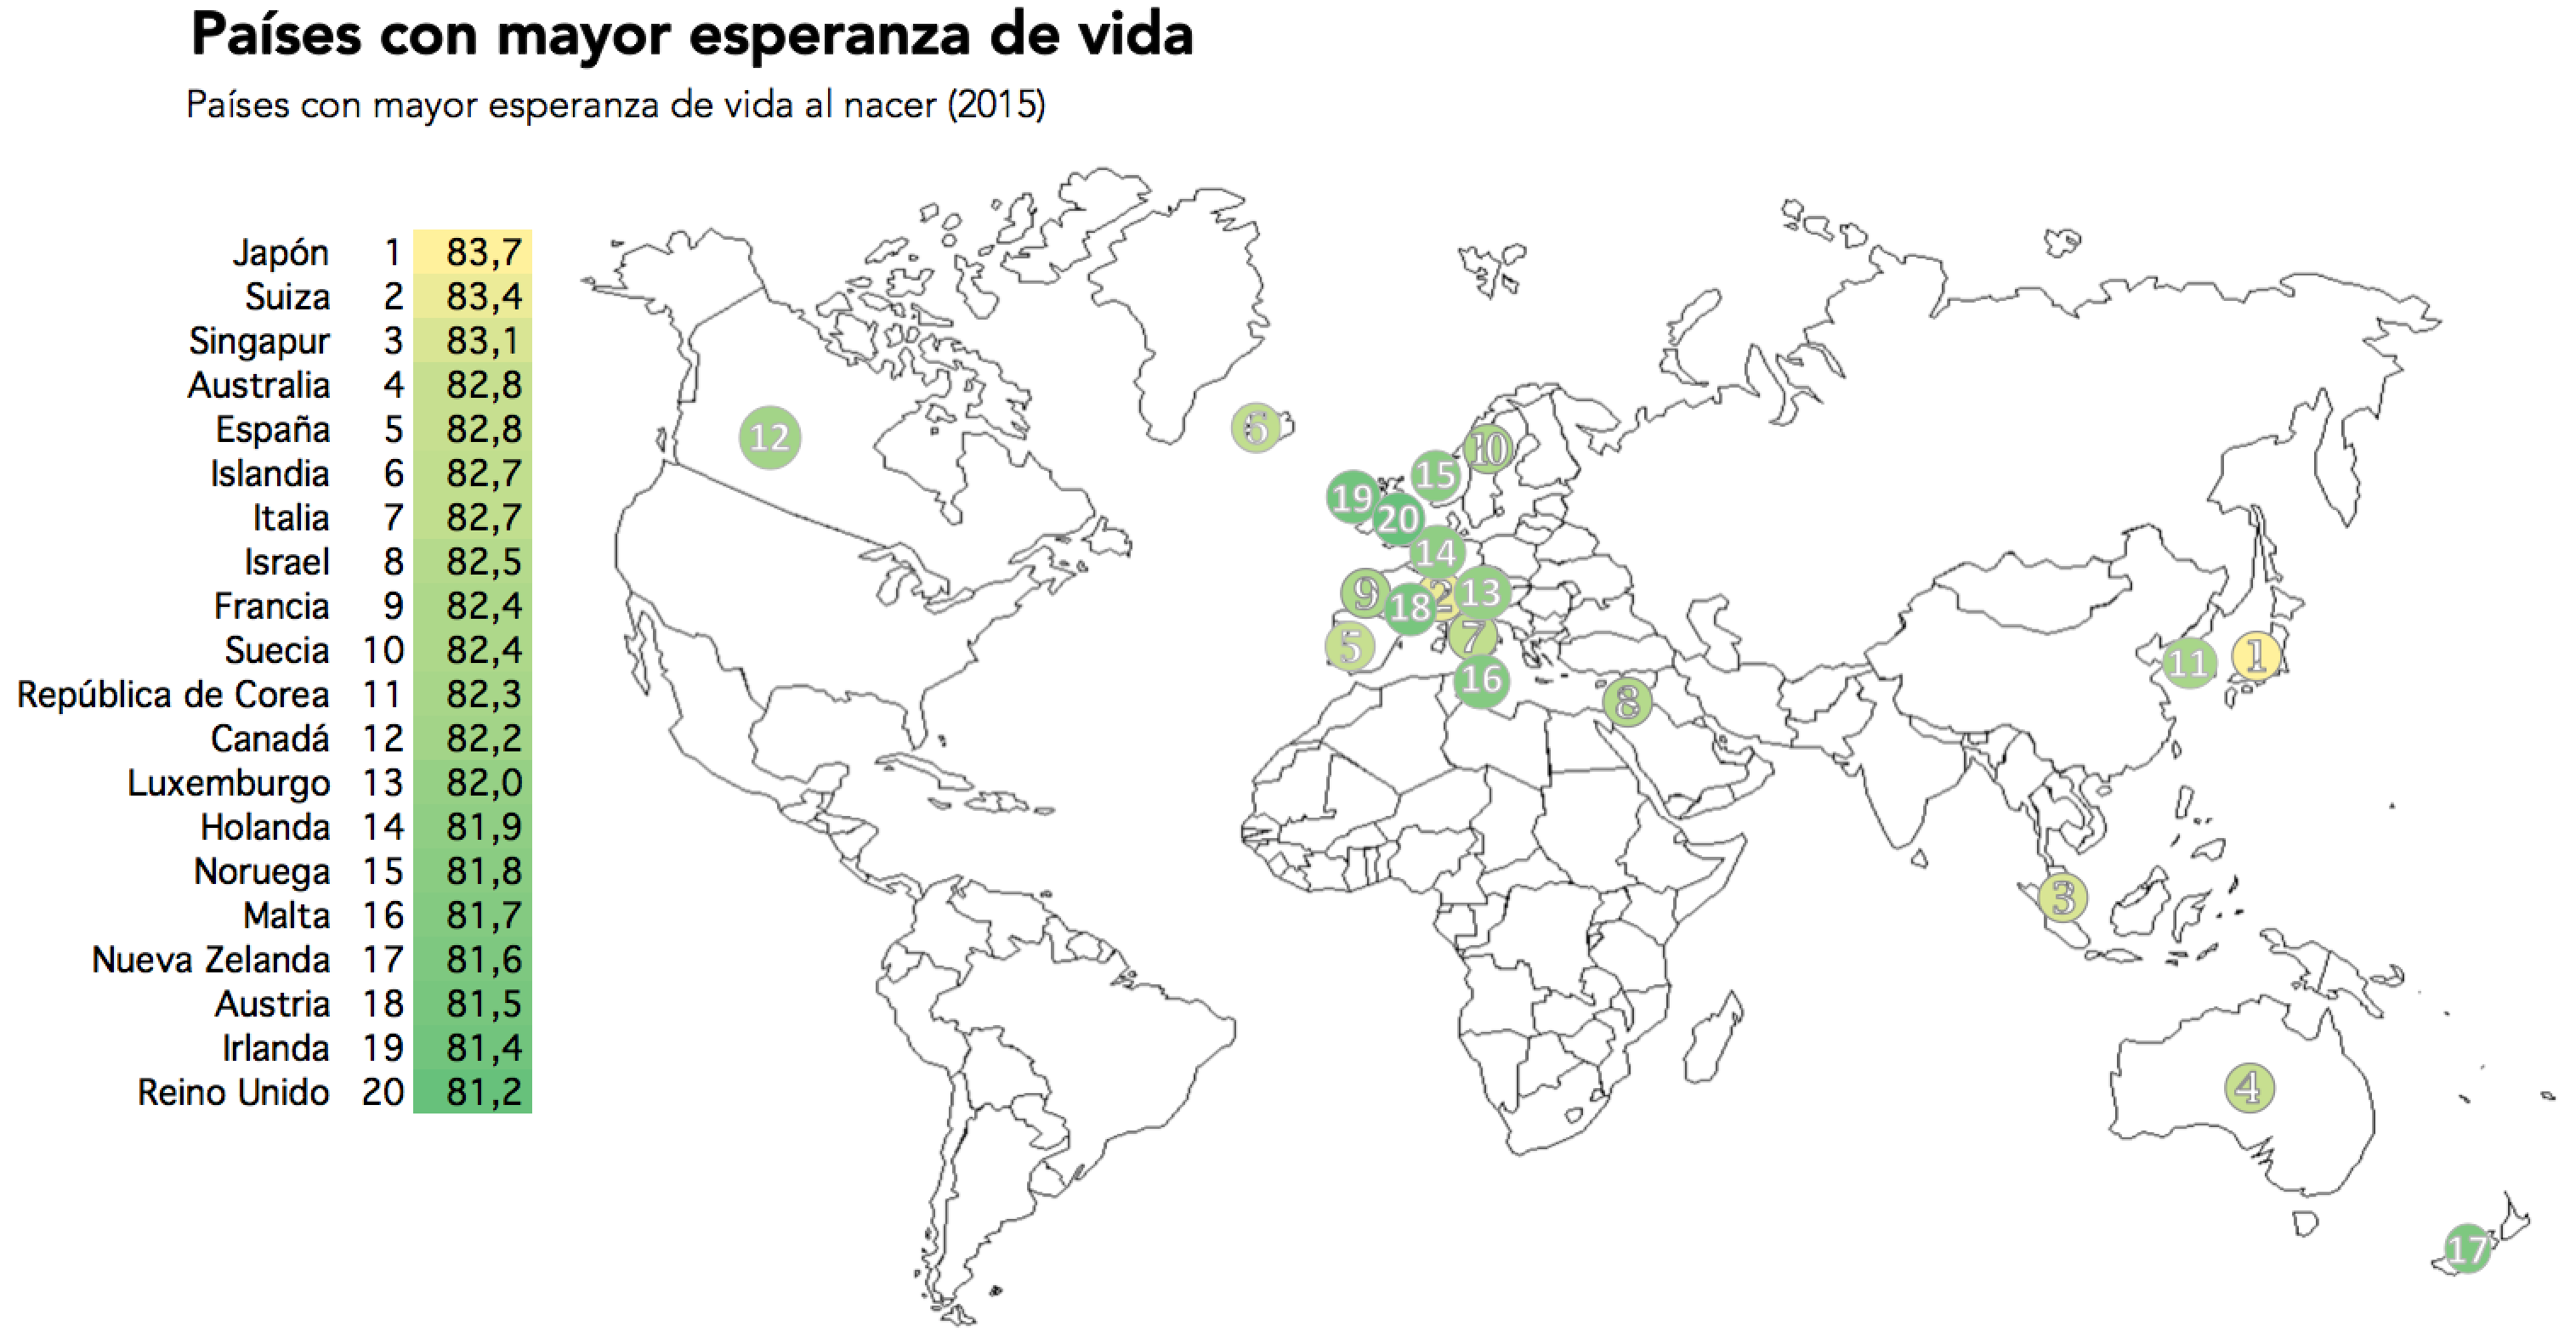
\includegraphics[scale=0.33]{Cap1/lifeexpectancy.png}
\caption{Pa\'ises con mayor esperanza de vida al nacer}\\
\textit{(Fuente: Elaboraci\'on propia a partir del Ministerio de Empleo y Seguridad Social)}
\end{figure}

Hace poco (concretamente en febrero de este año), \textit{Bloomberg}\footnote{\texttt{\small{\https://www.bloomberg.com/news/articles/2019-02-24/spain-tops-italy-as-world-s-\\healthiest-nation-while-u-s-slips}}} public\'o el índice de las naciones más saludables y de los diez países de los 169 que conforman el análisis, seis de ellos son europeos \textbf{(figura 1.13)}.
%\newpage
\begin{figure}[!ht]
\centering
\hspace*{0.0cm}\fbox{
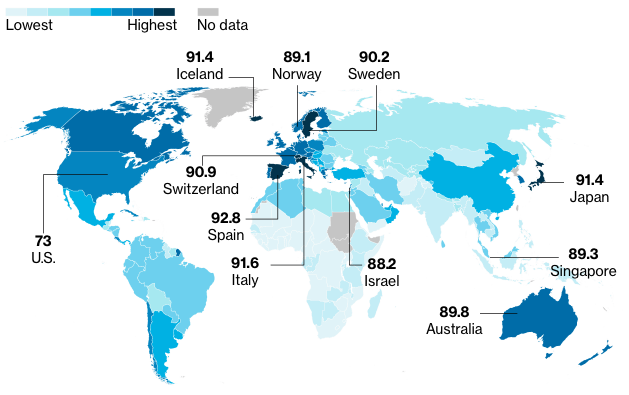
\includegraphics[width=15.5cm, height=8.5cm]{Cap1/healthiest.png}} %[scale=0.65]
\caption{Índice de salud global según Bloomberg con el top 10 (más los EEUU) señalados}\\
\textit{(Fuente: Bloomberg)}
\end{figure}

\vspace{-0.3cm}
Este índice contempla tanto la esperanza de vida (penalizando los riesgos provocados por el uso del tabaco y la obesidad) como factores medioambientales, incluyendo el acceso a agua potable y sanidad.\\

\vspace{-0.3cm}
España, que en 2017 se encontraba en el sexto lugar, ha escalado hasta la primera posición, superando a Italia, Japón e Islandia, por lo tanto, se puede decir que España es el país \textit{más saludable del mundo}, (los Estados Unidos aparecen en la 35\textsuperscript{a} posición).\\

\vspace{-0.3cm}
Hace dos a\~nos y medio, durante el discurso sobre el Estado de la Unión, el presidente de la Comisión Europea, Jean-Claude Juncker, se lamentaba diciendo: \textit{``el mundo es cada vez mayor y nosotros somos cada vez más pequeños''}. Se refería a que a medida que países como China, Brasil o India ganan peso, en todos los sentidos, en el panorama global, según las previsiones, en el 2050 (posiblemente ya sin el Reino Unido entre sus miembros), la Unión Europea representará el 5\% de la población total. Según datos del Eurostat\footnote{\texttt{\small{https://ec.europa.eu/eurostat/documents/2995521/9648811/3-12032019-AP-EN.pdf/\\412879ef-3993-44f5-8276-38b482c766d8}}}. En la actualidad, según este informe, hoy día, la UE supone el 7\% de los habitantes del planeta (en 1965 era el 13\%).\\

\vspace{-0.3cm}
Con todo, la creciente longevidad, medida como el aumento de la esperanza de vida en la edad del nacimiento o de la jubilaci\'on, supone un desaf\'io para los sistemas de pensiones en el \'ambito mundial. El aumento de la longevidad prolonga el periodo de percepci\'on de las retribuciones de las pensiones y, por lo tanto, aumenta las exigencias financieras de los sistemas de pensiones, ya sean de capitalizaci\'on individual o de reparto. Sin embargo, los cambios que implica una mayor longevidad van m\'as all\'a y afectan de forma general a todas las instituciones y en particular a las pensiones p\'ublicas (Ayuso y Holzmann, 2014) \textcolor{red}{[12]}.\\

\vspace{-0.3cm}
Para la mayor parte de los expertos del mundo hay una certeza; el sistema actual de pensiones en el mundo desarrollado explotar\'a; la cuesti\'on estriba  solo en saber cu\'ando lo har\'a.\\
El aumento del nivel de vida y la ca\'ida de la fertilidad a lo largo y ancho del mundo terminar\'an haciendo que los actuales sistemas de pensiones no sean sostenibles. Los expertos de Citigroup han publicado un informe al respecto \textcolor{red}{[13]} y la conclusi\'on es clara: \textit{las pensiones dentro de unos a\~nos no ser\'an como hasta ahora, ser\'an m\'as bajas y las cobrar\'an jubilados que trabajar\'an m\'as a\~nos}.\\

\vspace{-0.3cm}
Cuando naci\'o el primer sistema de pensiones, explican los analistas, la idea no era proporcionar un retiro confortable a los trabajadores, sino otorgar alguna protecci\'on para evitar la pobreza a los mayores. Con el tiempo esta idea evolucion\'o hasta un sistema que para estos expertos tendr\'a que dejar de ser lo que es ahora para convertirse en algo m\'as parecido a lo que fue cuando se concibi\'o. Para entender de d\'onde nace el concepto de crisis, bastan algunas cifras:\\

\vspace{-0.3cm}
\noindent \textbf{\checkmark}  Cuando se confeccionaron los sistemas de pensiones, hace un siglo aproximadamente, la esperanza de vida en los pa\'ises desarrollados era de 51 a\~nos, ahora se ha elevado en unos 20 a\~nos. Esto quiere decir que los jubilados reciben pensiones alrededor de un 50\% m\'as de tiempo que cuando fueron originados. \\

\vspace{-0.3cm}
\noindent \textbf{\checkmark}  En Europa, el aumento de la esperanza de vida y la ca\'ida de natalidad ha hecho que el n\'umero de europeos mayores de 65 a\~nos sea del 17\% de la poblaci\'on; previsiblemente, en 2050 esa cifra alcanzar\'a el 26\%. En China, se espera que pase del 12\% actual, al 24\% en 2050.

%\newpage
\begin{figure}[!ht]
\hspace*{-0.6cm}
\begin{minipage}{.55\textwidth}
  \centering
\vspace{-0.3cm}\fbox{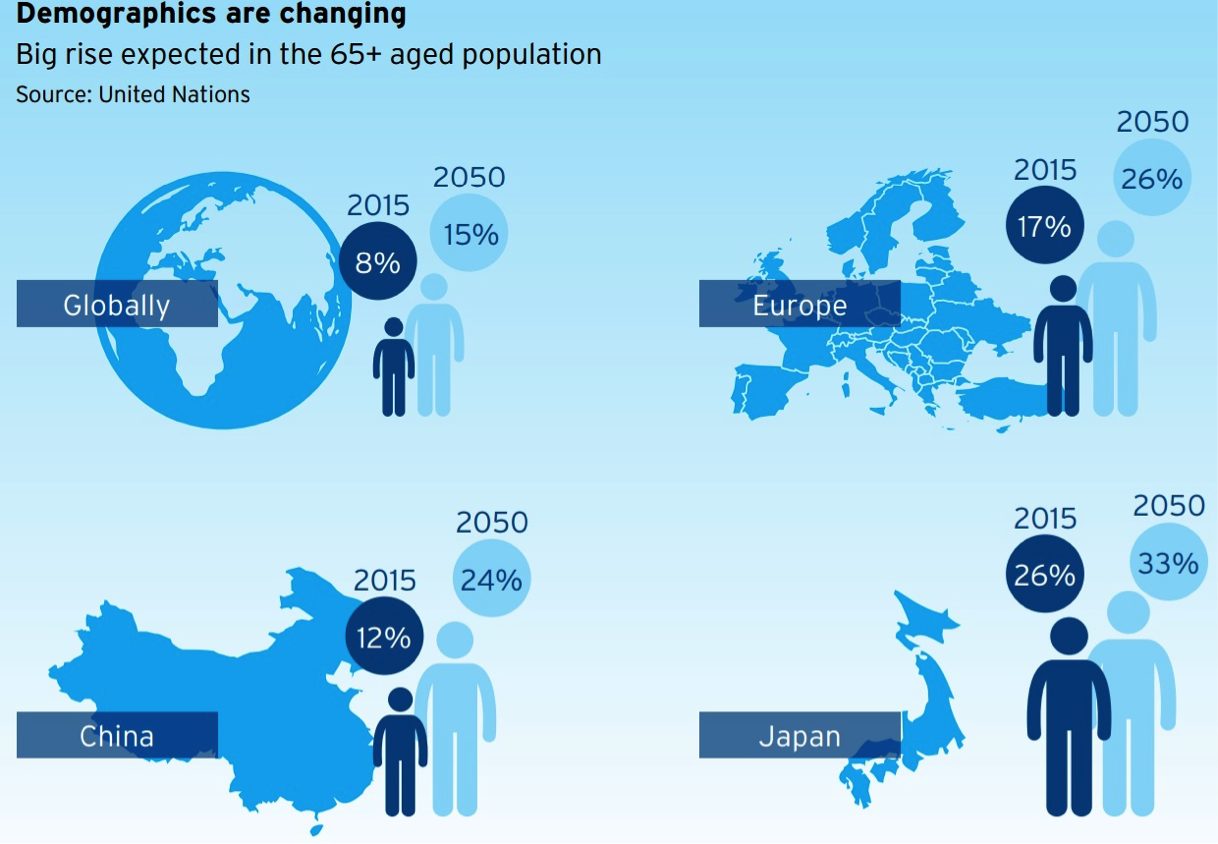
\includegraphics[width=3.4in,height=2.5in]{Cap1/ingles1.png}}
 %\parbox{10cm}
\captionsetup{width=0.9\linewidth}
\caption[\% de crecimiento esperado en la poblaci\'on de 65 o m\'as a\~nos 2015 vs 2050]{Crecimiento esperado (en \%) en la poblaci\'on de 65 o m\'as a\~nos 2015 vs 2050.\\ {\small\textit{(Fuente: Naciones Unidas)}}}
\end{minipage}%
\begin{minipage}{.5\textwidth}
\vspace{-0.2cm}\fbox{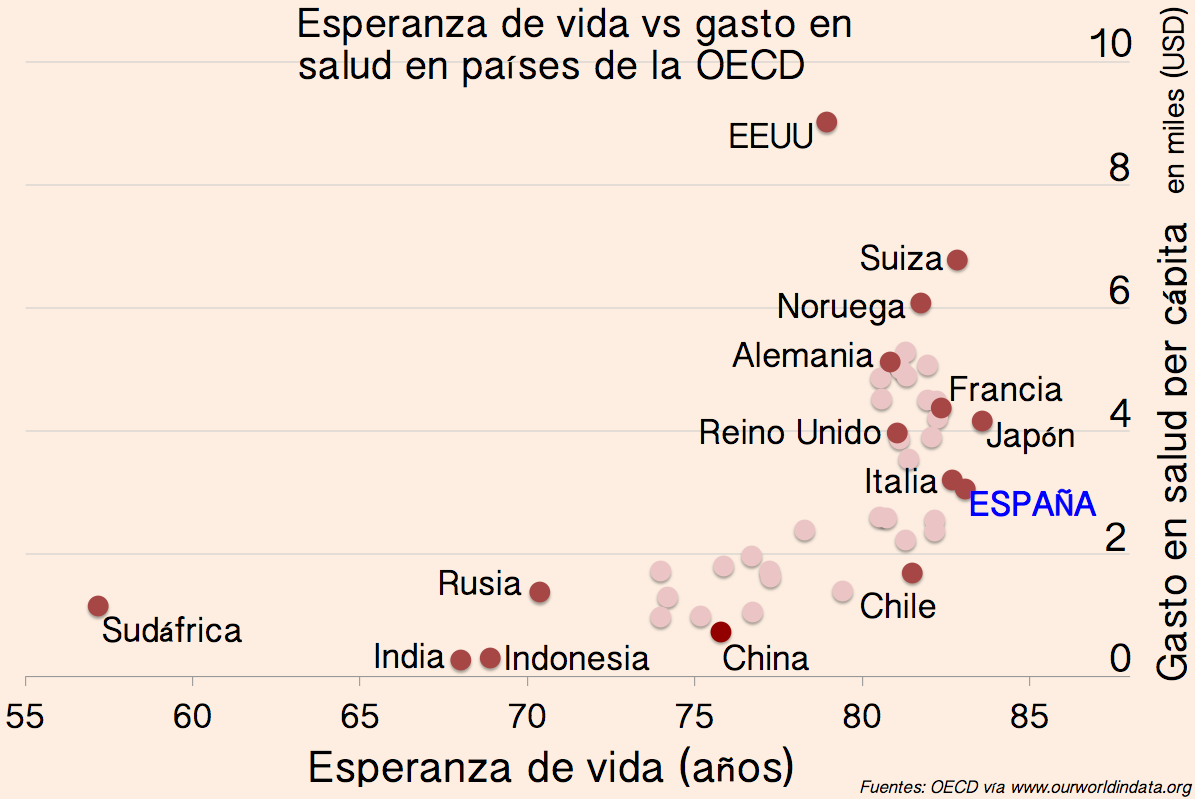
\includegraphics[width=3.4in,height=2.5in]{Cap1/oecd.png}}
%\parbox{8cm}
\captionsetup{width=1\linewidth}
\hspace*{0.8cm}
\vspace{-0.3cm}
\caption[Esperanza de vida vs. gasto en salud en países OECD]{Esperanza de vida vs. gasto en salud en países OECD.\\ {\small\textit{(Fuente: OECD v\'ia www.ourworldindata.org)}}}
\end{minipage}
\end{figure}
%\begin{figure}[!ht]
%\centering
%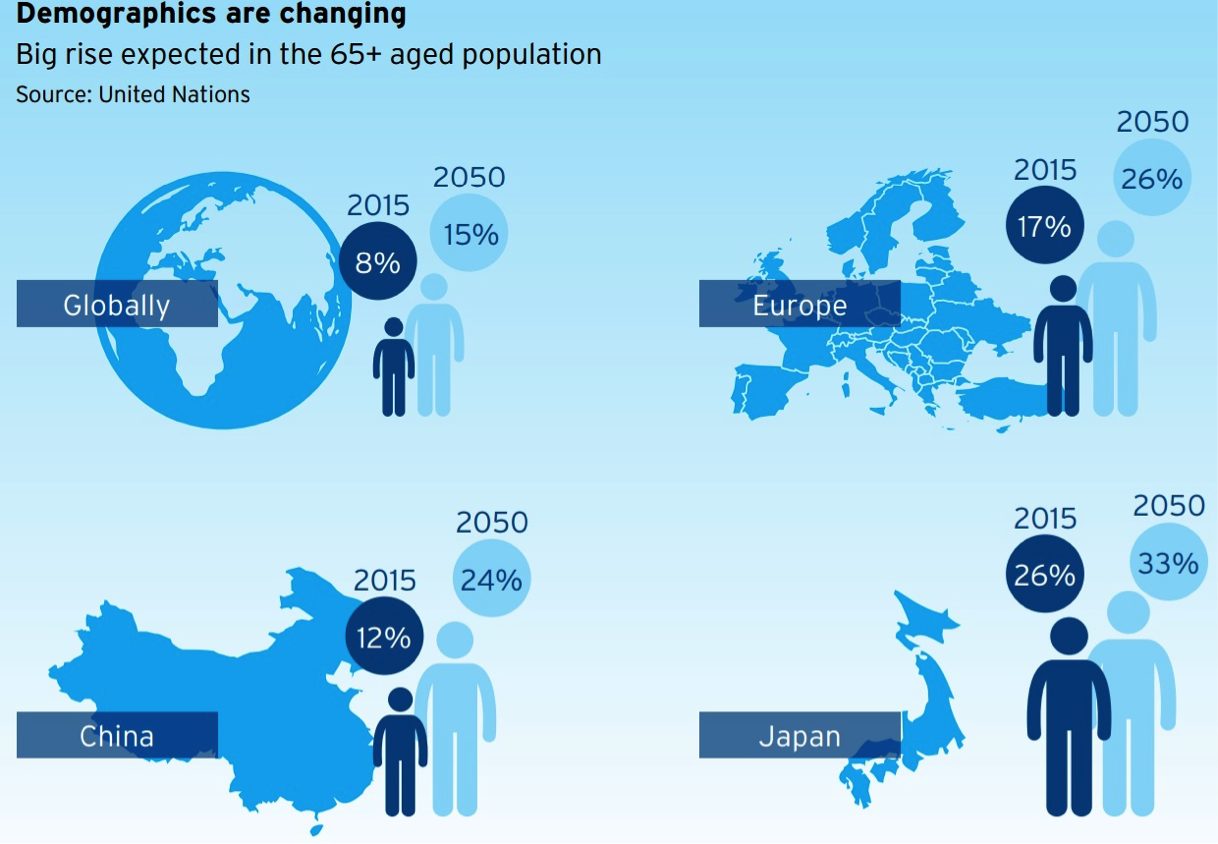
\includegraphics[scale=0.6]{Cap1/ingles1.png}
%\caption{Crecimiento esperado (en \%) en la poblaci\'on de 65 o m\'as a\~nos 2015 vs 2050}\\
%\textit{\small{(Fuente: Naciones Unidas)}}
%\end{figure}
%\begin{figure}[!ht]
%\centering
%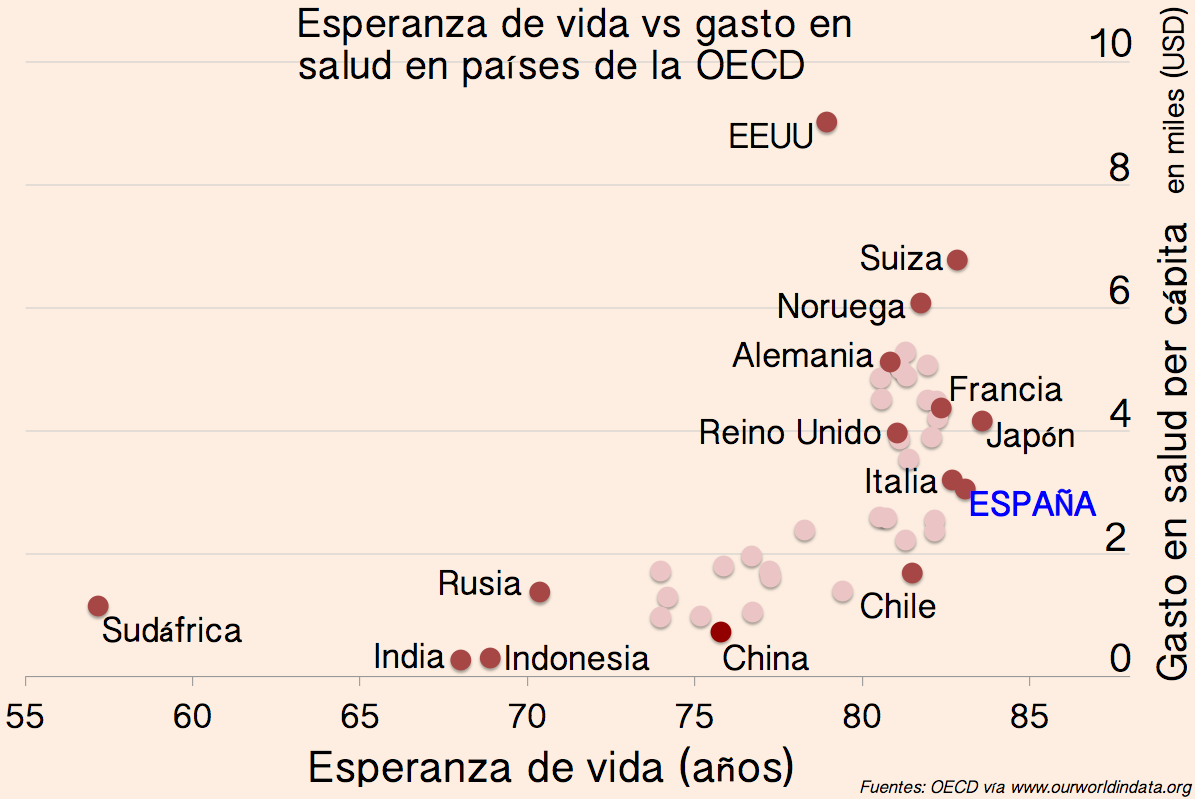
\includegraphics[scale=0.35]{Cap1/oecd.png}
%\caption{Esperanza de vida vs. gasto en salud en pa\'ises de la OECD}\\
%\textit{\small{(Fuente: OECD v\'ia www.ourworldindata.org)}}
%\end{figure}
\vspace{-0.5cm}

\noindent \textbf{\checkmark} Italia y Espa\~na se convertir\'an en el segundo y el tercer pa\'is m\'as envejecidos del mundo, respectivamente, con apenas dos habitantes en edad de trabajar por cada jubilado, lo que da la imagen de que no ser\'a suficiente para pagar las pensiones. En la actualidad en Espa\~na, los trabajadores financian el pago a los actuales pensionistas, no guardan dinero para su jubilaci\'on.\\

\begin{wrapfigure}[18]{r}{0.5\textwidth}
\centering
\vspace{-1cm}
\hspace*{-2.5cm}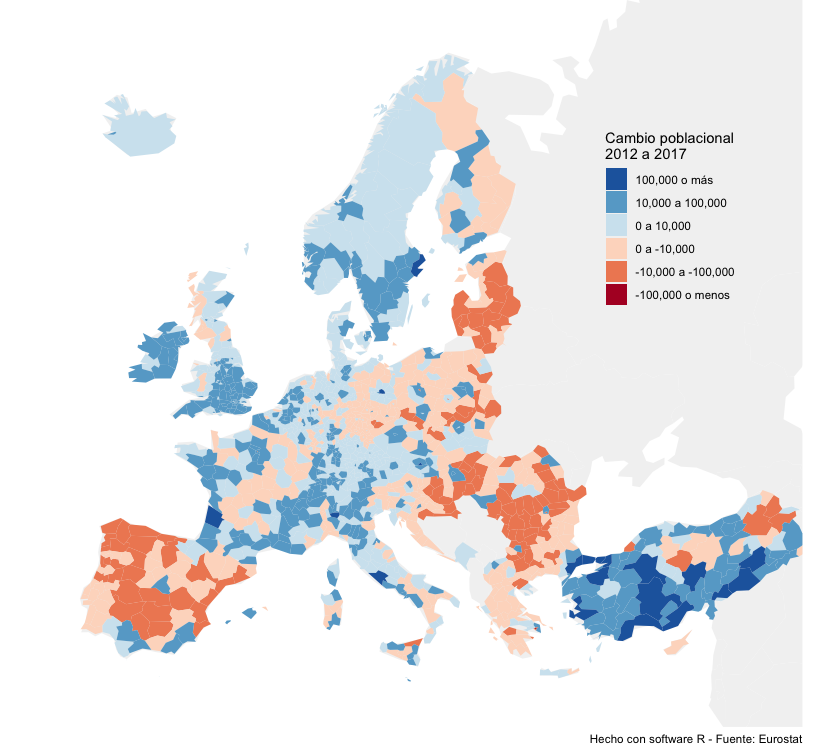
\includegraphics[width=0.65\textwidth]{Cap1/eurostat.png}
\captionsetup{width=1.2\linewidth}
\caption{\label{fig:frog1}Fuente: Elaboraci\'on propia a partir de datos de la OECD} 
%\hspace{-0.65cm}\textit{\small{(Fuente: Elaboraci\'on propia a partir de datos de la OECD)}}
\end{wrapfigure}
En la \textbf{figura 1.16} se muestra el cambio poblacional que ha tenido lugar en los pa\'ises de Europa (con sus respectivas regiones) desde el a\~no 2012 hasta el a\~no 2017; en esos cinco a\~nos se observa que mientras en la mayor\'ia de los pa\'ises del centro y del norte de Europa la poblaci\'on se ha incrementado (aunque haya regiones donde apenas ha disminuido), en Espa\~na  y en los pa\'ises del este, el cambio poblacional ha sido negativo, es decir, la poblaci\'on ha disminuido. Particularmente llamativo es el caso de Turqu\'ia donde exceptuando algunas regiones del norte y del este, el resto del pa\'is ha experimentado el cambio poblacional m\'as elevado de Europa. En estos momentos, adem\'as, los sistemas p\'ublicos de pensiones no tienen suficiente dinero guardado como para hacer frente a los pagos que tendr\'an que hacer en un futuro.\\ 
Algo que afecta sobre todo a Europa, donde predominan los sistemas p\'ublicos, frente a los privados. Aseguran que en el viejo continente ``el coste de estos compromisos ser\'ia m\'as del doble a la deuda p\'ublica''. Como resultado, en el futuro, los ciudadanos van a experimentar -seg\'un los expertos- \textit{`presiones econ\'omicas y empobrecimiento de sus niveles de vida'}.
%\end{itemize}
%\newpage

\noindent \textbf{\checkmark} Hay que tener en cuenta que, adem\'as, el dinero de las pensiones se invierte actualmente mayoritariamente en renta fija y que la rentabilidad de este tipo de activos se ha hundido en las \'ultimas d\'ecadas, con lo que estamos ante un nuevo reto para los gestores.\\

La \textbf{figura 1.17} es un claro ejemplo de lo explicado anteriormente; en el pasado y presente, gobiernos y empresas privadas de la mayor\'ia de los pa\'ises industrializados, han asumido importantes compromisos que se extienden a lo largo de d\'ecadas en el futuro, pero en su mayor\'ia no han conseguido aportar suficientes fondos para cumplir esos compromisos. Seg\'un el citado informe de Citigroup, se calcula que de media, en 20 de los pa\'ises de la OCDE, habr\'ia un d\'eficit para los pr\'oximos a\~nos de unos 78 billones de d\'olares que no aparecen en los balances de esos estados.
\vspace{-0.2cm}
\begin{figure}[H]
\centering
\fbox{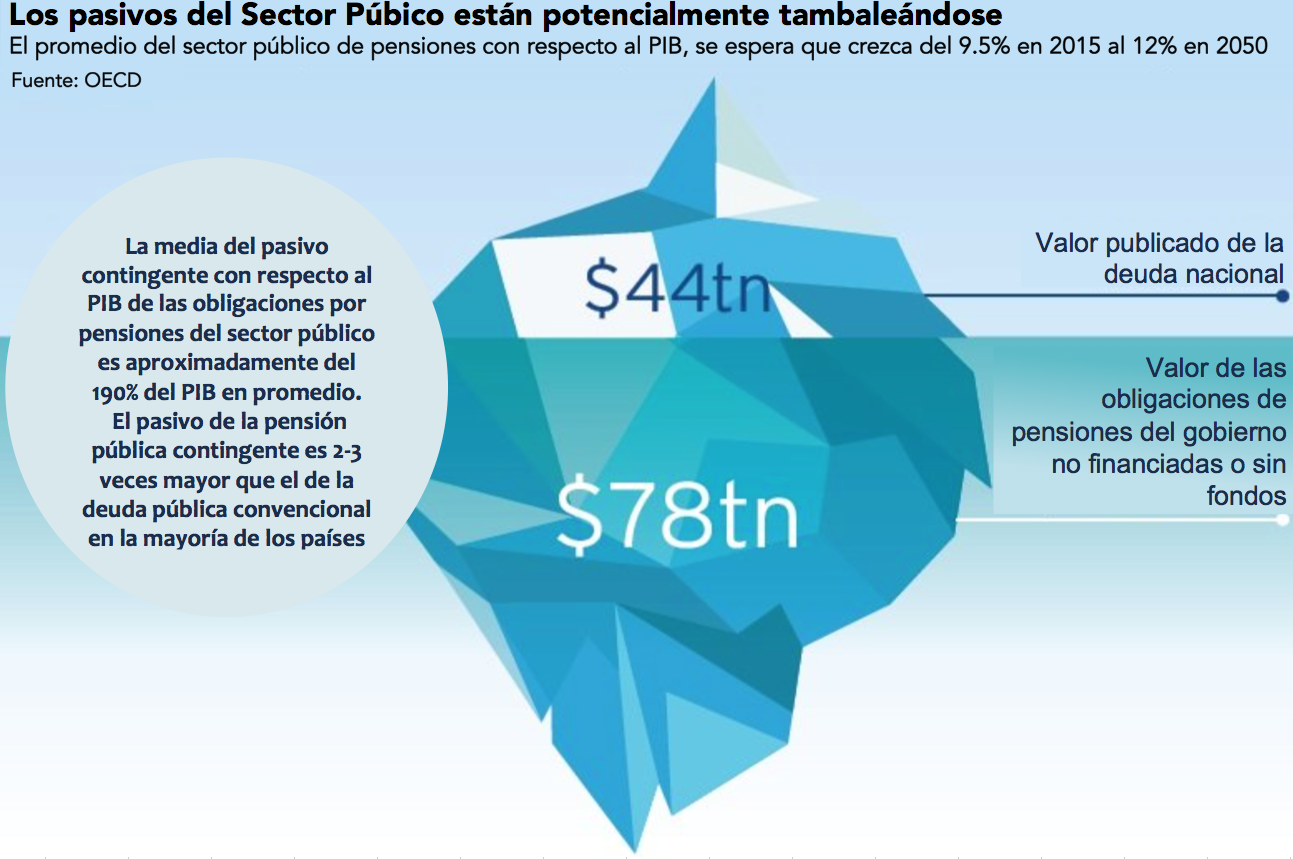
\includegraphics[scale=0.28]{Cap1/ingles2a.png}}
\vspace{-0.25cm}
\caption[Comparativa entre el valor de la deuda nacional publicada y el d\'eficit calculado en las pensiones]{Comparativa entre el valor de la deuda nacional publicada y el d\'eficit calculado en las pensiones a las que los gobiernos tendr\'an que hacer frente en los pr\'oximos a\~nos}\\
\textit{\small{(Fuente: OCDE v\'ia www.businessinsider.com)}}
\end{figure}
Desde una perspectiva compleja, dicha cantidad es casi el doble de la deuda pendiente del gobierno de esas mismas naciones, la cual es alrededor de 44 billones de d\'olares. La forma de representar este dato en el informe suministrado por Citigroup es significativa y simb\'olica, ya que muestra la escala del problema inminente que acecha bajo la superficie y que gobiernos y corporaciones.\\

El uso de un iceberg es, claramente sintom\'atico del problema al que corporaciones y gobiernos por igual se enfrentan en el futuro. Seg\'un el informe, \textit{``si la representaci\'on no es lo suficientemente ``aterradora'' como para estremecernos''}, \textit{Citigroup} lo refleja en palabras: \textit{``si nos centramos en los pasivos de las pensiones del gobierno para los trabajadores del sector p\'ublico y la Seguridad Social, el an\'alisis de estos veinte pa\'ises de la OCDE indica un nivel promedio de pasivos por pensiones del gobierno sin fondos del 190\% del PIB. Para ese mismo grupo de pa\'ises, la cantidad reportada de todas las deudas del gobierno asciende solo al 109\% del PIB. En t\'erminos de d\'olares estadounidenses, estimamos que la falta de fondos para la jubilaci\'on a nivel global establecidos en los balances del gobierno de estos veinte países asciende a 78 trillones de USD, en comparaci\'on con las deudas nacionales reportadas que totalizan 44 trillones de USD. Por lo tanto, si se agregan los pasivos de la Seguridad Social y la falta de financiaci\'on de los trabajadores del sector p\'ublico como una forma de ``deuda contingente'', la deuda total del gobierno mundial puede ser tres veces m\'as grande de lo que la gente cree actualmente. Cualquiera que sea el c\'alculo utilizado, los n\'umeros son asombrosos. Eso equivaldr\'ia a una proporci\'on de deuda p\'ublica/PIB de m\'as del 300\%, lo que hace que la deuda del gobierno japon\'es sea similar.} Como sugiere \textit{Citigroup}, las matem\'aticas son simples, las soluciones no tanto.\\ 

\textit{``El mundo se enfrenta a una crisis de jubilaci\'on''}, dice el banco; todas estas cifras hacen pensar a los expertos que hay que hacer algo y pronto, para evitar el cataclismo. Sin embargo, las soluciones y las oportunidades est\'an disponibles si los gobiernos y las corporaciones toman medidas para comenzar a abordar los problemas. Estas conversaciones y acciones deben comenzar ahora y se requiere la participaci\'on de todas las partes para garantizar que no se produzca un desastre fiscal en las pr\'oximas d\'ecadas.\\ 

\vspace{-0.3cm}
En este sentido, estas son las soluciones que sugieren en la entidad:\\

\vspace{-0.3cm}
\noindent \textbf{1)} Calcular cu\'al ser\'a la cantidad que tendr\'an que pagar los estados cada a\~no y hacerla p\'ublica (derechos de cobro reconocidos). En su opini\'on, es la \'unica opci\'on que tendr\'an los pol\'iticos para poder afrontar el problema de las pensiones.  Los c\'alculos, adem\'as, tendr\'an que seguir unos criterios claros que deber\'ian establecer instituciones como la Uni\'on Europea, el FMI o la OCDE.\\

\vspace{-0.3cm}
\noindent \textbf{2)} Vincular la edad de la jubilaci\'on a la esperanza de vida. Ellos creen que si se volviera a los inicios y los pensionistas cobrar\'an por un espacio de tiempo de 12 a\~nos, la nueva edad para retirarse tendr\'ia que elevarse hasta los 73 a\~nos.\\

\vspace{-0.3cm}
\noindent \textbf{3)} A los europeos les recomienda volver a redise\~nar el concepto de jubilaci\'on y relacionarlo a un pago que solo cubra las necesidades b\'asicas, tal y como se concibi\'o hace un siglo. Recuerda que hay pa\'ises como Espa\~na en el que los pagos en los pr\'oximos a\~nos triplicar\'an el PIB.  En opini\'on, \textit{``la idea de que los gobiernos deben garantizar ingresos a los mayores durante m\'as de 25 a\~nos no es sostenible en nuestra opini\'on''}, dicen desde fuentes consultadas.  En estos momentos, los pagos a pensiones en Espa\~na rondan ya el 10\% del PIB y alcanzar\'a el 15\% en los pr\'oximos a\~nos.

\begin{figure}[!ht]
\centering
\fbox{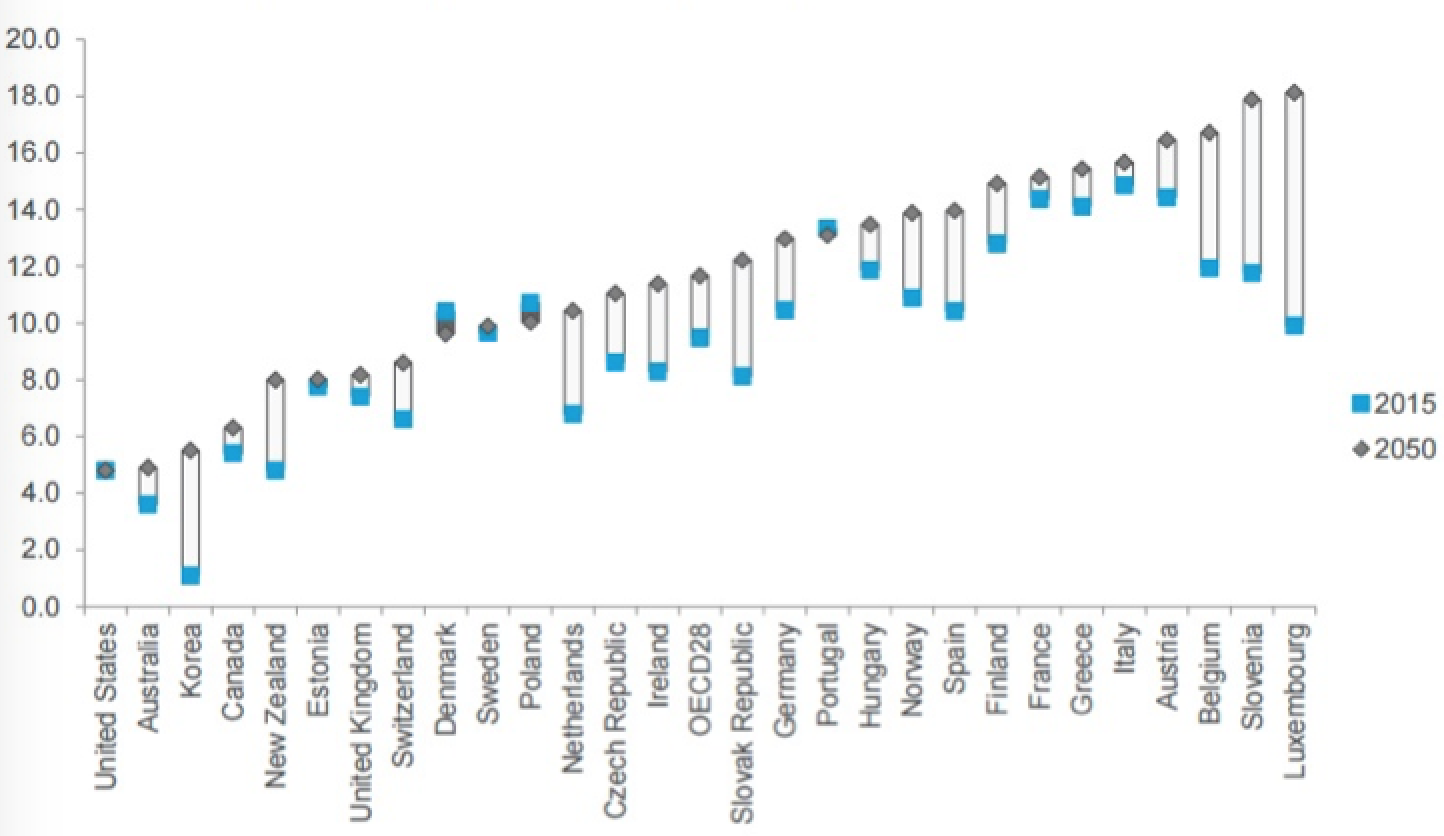
\includegraphics[scale=0.48]{Cap1/ingles3.png}}
\caption[Estimaci\'on del pago del Gobierno en pensiones 2015 a 2050 en proporci\'on del PIB]{Estimaci\'on del pago del Gobierno en pensiones 2015 a 2050 en proporci\'on del PIB (variaciones en los costes por pensi\'on del sector p\'ublico por pa\'is)}\\
\textit{\small{(Fuente: OCDE - Citi Research)}}
\end{figure}

%\vspace{-0.3cm}
\noindent \textbf{4)} Adoptar nuevos sistemas como el holand\'es en los que se establece  un modelo mixto (p\'ublico y privado). El estado ofrece una red de seguridad p\'ublica a todos los trabajadores y que luego hace descansar en \'estos la decisi\'on de la cuant\'ia que desean obtener a la hora de su jubilaci\'on. El estado solo les garantiza una pensi\'on equivalente al salario m\'inimo. Adem\'as, luego pueden acceder a un sistema privado al que se pueden acoger empresas y trabajadores.\\

\vspace{-0.3cm}
\noindent \textbf{5)} Incentivar fiscalmente los planes de pensiones privados y favorecer los planes de pensiones dentro de las empresas.\\

\vspace{-0.3cm}
\noindent \textbf{6)} Proteger a los consumidores en t\'erminos de costes y de regulaci\'on.\\

\vspace{-0.3cm}
\noindent \textbf{7)} Asegurarse que todos los trabajadores tienen acceso a un plan de pensiones en su trabajo.\\

\vspace{-0.3cm}
\noindent \textbf{8)} Solucionar, con una perspectiva de largo plazo, los d\'eficits de los sistemas p\'ublicos de pensiones.\\

\noindent Recientemente, se ha tratado de determinar si los esfuerzos del gobierno en la reducci\'on de las desigualdades en la salud en los pa\'ises europeos han provocado diferencias en las desigualdades de mortalidad por grupo socioecon\'omico. Este estudio, (Mackenback, 2014) \textcolor{red}{[14]}, se realiz\'o para todos aquellos pa\'ises europeos en los cuales los datos sobre desigualdades sociecon\'omicas en mortalidad estaban disponibles entre los a\~nos 1990 y 2010, incluyendo pa\'ises como Finlandia, Noruega, Suecia, Reino Unido (Escocia, Inglaterra y Gales), Francia, Suiza, Espa\~na, Italia, Eslovenia y Lituania.\\
Las conclusiones b\'asicas fueron que durante las \'ultimas dos d\'ecadas, la evoluci\'on de las desigualdades en la mortalidad han sido más favorables en la mayor\'ia de los pa\'ises europeos de lo que com\'unmente se supone. Las desigualdades absolutas han disminuido en varios pa\'ises, probablemente m\'as como un efecto secundario de los cambios de comportamiento en toda la poblaci\'on as\'i como mejoras en la prevenci\'on y el tratamiento, que como un efecto de las pol\'iticas destinadas expl\'icitamente a la reducci\'on de las desigualdades en salud.

\begin{figure}[!ht]
\centering
\fbox{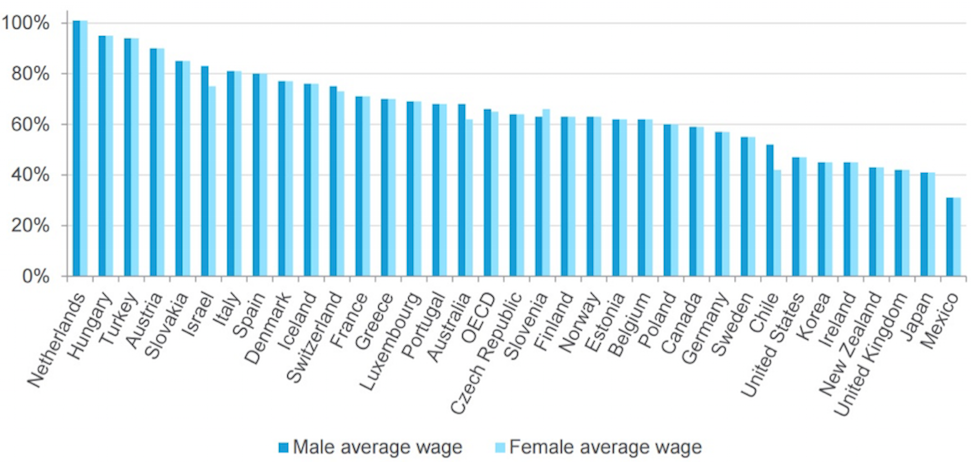
\includegraphics[scale=0.38]{Cap1/ingles4.png}}
\caption{Tasas de sustituci\'on de la pensi\'on masculina y femenina, 2017}\\
\small{(Fuente: OECD - Citi Research)}
\end{figure}

Las consecuencias de tal envejecimiento poblacional, como apunta la ONU en sus previsiones demogr\'aficas para las pr\'oximas d\'ecadas, advierten sobre un fuerte retroceso vegetativo y envejecimiento poblacional en los pa\'ises m\'as desarrollados. En concreto, seg\'un apuntan las principales conclusiones del estudio publicado en la revista de la \textit{National Academy of Sciences} de Estados Unidos, (Raftery, 2012) \textcolor{red}{[15]} y que advierte sobre las consecuencias económicas de un fen\'omeno a escala mundial, en en China por ejemplo, el n\'umero de adultos en edad de trabajar por cada persona mayor de 65 a\~nos se reducir\'a de los 7,9 actuales a 1,6 en 2100, mientras que en la India, la misma proporci\'on pasar\'a de 11,1 a 2,00.


%%%%%%%%%%%%%%%%%%% SECCION 1.4.: CONSECUENCIAS ECONÓMICAS, SOCIALES.... %%%%%%%%%%%%%%%%%%

\section{Consecuencias econ\'omicas, sociales y geopol\'iticas de los desequilibrios demogr\'aficos: algunas teor\'ias (pocas) y evidencias (muchas).}

Las consecuencias del continuo crecimiento de la poblaci\'on siempre han sido objeto de `encendidos' temas de debate, especialmente desde un punto de vista te\'orico, donde dos corrientes opuestas en sus fundamentos han tratado de explicar la naturaleza y consecuencias de las influencias demogr\'aficas. Sin extendernos demasiado en estas dos \textit{``teor\'ias''}, se\~nalaremos que la primera, desarrollada en los a\~nos 30 y  denominada \textbf{\textit{teor\'ia del estancamiento}},\footnote{En ingl\'es, la  ``teor\'ia del estancamiento secular'' \textit{(secular stagnation theory)}, fue se\~nalada en los trabajos de Alvin Hansen (1939) para describir un periodo prolongado de lento crecimiento econ\'omico acompa\~nado de altas tasas de desempleo.} percibe el crecimiento demogr\'afico como un est\'imulo para el desarrollo econ\'omico. Seg\'un Hansen, 1939 \textcolor{red}{[16]}: \textit{``los economistas formados en la tradici\'on de la teor\'ia malthusiana piensan en t\'erminos est\'aticos y tienden a dar al cese del crecimiento demogr\'afico una interpretaci\'on optimista''.} De hecho, las ideas de Hansen se apoyan en Adam Smith, quien se\~nala que el crecimiento de la poblaci\'on es causa y consecuencia del progreso econ\'omico. As\'i, para Hansen, el progreso econ\'omico consta de tres elementos: (i) invenciones; (ii) descubrimiento y explotaci\'on de tierra y nuevos recursos; y (iii) crecimiento de la poblaci\'on.\\

\vspace{-0.2cm}
De este modo, el crecimiento demogr\'afico en la segunda mitad del siglo XIX es responsable, aproximadamente, del 40\% del volumen total de la formaci\'on de capital en los pa\'ises de Europa del Oeste y del 60\% en los Estados Unidos, lo que confirma que las reducciones en las oportunidades de inversi\'on tienden a agravar las tensiones econ\'omicas y el desempleo en tanto que la demanda decae m\'as all\'a de las expectativas de los inversores.\\

\vspace{-0.2cm}
En cambio, la \textbf{\textit{teor\'ia neo-malthusiana}} concibe el crecimiento demogr\'afico como un obst\'aculo para el desarrollo econ\'omico, proponiendo que una disminuci\'on en las tasas de fertilidad acelera el crecimiento de los ingresos totales y especialmente el crecimiento de los ingresos por capital. Este razonamiento se basa en tres explicaciones posibles: la mejora en la productividad por trabajador; los recursos liberados por una disminuci\'on en el ratio de dependientes (debido a la ca\'ida en el n\'umero de nacimientos); y el incremento en los ahorros debido al crecimiento en el ingreso medio.\\

\vspace{-0.2cm}
La aproximaci\'on pr\'actica para la comprobaci\'on de estas teor\'ias, o m\'as bien para comprobar la relaci\'on entre poblaci\'on y crecimiento econ\'omico es la idea de Chesnais, (2013) \textcolor{red}{[17]}. Por ejemplo, a la hora de calcular la correlaci\'on entre el crecimiento de la poblaci\'on y los incrementos en ingresos per capita a precios constantes en un periodo determinado. Este estudio no fue todo lo concluyente como para confirmar alguna de las teor\'ias anteriormente descritas, habiendo una contradicci\'on entre los paradigmas te\'oricos y la realidad hist\'orica.\\

\vspace{-0.2cm}
De este modo, durante la primera mitad del periodo estudiado se observ\'o que mientras m\'as r\'apido se desarroll\'o el crecimiento demogr\'afico, el progreso econ\'omico tend\'ia a ser m\'as significante. Sin embargo, esta observaci\'on emp\'irica no se sostuvo para las siguientes d\'ecadas, donde pa\'ises con un r\'apido crecimiento de la poblaci\'on (por ejemplo, y principalmente, pa\'ises del \'Africa subsahariana) experimentaron los ingresos m\'as bajos en ingresos per c\'apita.\\
Siendo este el caso, el coeficiente de correlaci\'on entre las dos series de \'indices de crecimiento fue al principio positiva para luego volverse negativa y aunque la correlaci\'on era d\'ebil, parece que las diferencias en el crecimiento de la poblaci\'on no fueron tan determinantes a la hora de explicar los patrones del crecimiento econ\'omico.\\

\vspace{-0.2cm}
Sea como fuere, y m\'as all\'a de teor\'ias deterministas del crecimiento demogr\'afico propias de su tiempo, la actividad económica y las dinámicas poblacionales están estrechamente ligadas. Así, crecimiento econ\'omico y crecimiento demogr\'afico pueden reaccionar tanto positiva como negativamente a los mismos est\'imulos y la evolución demográfica afecta al crecimiento a medio y largo plazo, condicionando así aspectos tan importantes como el mercado laboral o las políticas de gasto relacionadas con la vejez (lo que afecta significativamente en la distribución de la riqueza inter-generacional). \\

\vspace{-0.2cm}
Según la AIReF \textcolor{red}{[18]}, las proyecciones demográficas que publican algunos organismos, si son acertadas, podrían cambiar la dinámica de indicadores macroeconómicos tales como las tasas de crecimiento reales del PIB, las aportaciones del capital o el crecimiento de la productividad.\\

\vspace{-0.2cm}
\noindent \textbullet\ El \textbf{crecimiento de la poblaci\'on incrementa la presi\'on sobre los recursos naturales}, limitando, por ejemplo la tierra o el espacio f\'isico. En el terreno de la agricultura esto, significa una disminuci\'on de la superficie media de tierra cultivable de acuerdo con la ley de los rendimientos decrecientes.\\

\vspace{-0.2cm}
\noindent \textbullet\ Una \textbf{alta fertilidad} obliga a la mayor\'ia de la poblaci\'on a dedicar su tiempo y energ\'ia a criar ni\~nos, por lo que el trabajo productivo fuera del hogar se reduce notablemente, especialmente entre las mujeres.\\

\vspace{-0.2cm}
\noindent \textbullet\ El \textbf{grado de inversi\'on necesario} para garantizar los mismos est\'andares de vida a miembros adicionales de la poblaci\'on es que el potencial para la formaci\'on de capital p\'ublico y privado se reduce notablemente. Una tasa de aumento demogr\'afico del 3\%, por ejemplo, absorber\'a del 9\% al 12\% del ingreso nacional, donde la relaci\'on de aumento de capital-producci\'on es 3 \'o 4. Esto conlleva a una disminuci\'on en la inversi\'on por trabajador, que en cambio afecta a mejoras en la productividad. Por el contrario, en los Estados Unidos, por ejemplo, la contracci\'on del coste educativo, por un lado, y el aumento del capital humano y no humano, por otro, han sido casi sim\'etricos.\\

\vspace{-0.2cm}
\noindent \textbullet\ A \textbf{nivel industrial}, la consecuencia m\'as directa del incremento demogr\'afico sobre el crecimiento econ\'omico es que bajo favorables circunstancias, la industrializaci\'on puede convertir el crecimiento demogr\'afico en un est\'imulo para incrementar el nivel de vida, tanto al obtener mano de obra para explotar los recursos naturales como para ampliar los mercados necesarios para absorber y rentabilizar los resultados de la producci\'on en masa. Es decir, el aumento demogr\'afico puede afectar la oferta y la demanda de los agentes econ\'omicos.\\

\vspace{-0.2cm}
\noindent \textbullet\ \textbf{Geogr\'afica y pol\'iticamente}, las repercusiones de una poblaci\'on envejecida tienen un impacto que afecta, dependiendo de la intensidad con que el proceso de desarrollo demogr\'afico se despliegue, al resto de estamentos y sectores de cualquier pa\'is.\\
A nivel pol\'itico, el envejecimiento demogr\'afico lleva unido un envejecimiento de la masa electoral, lo cual explicar\'ia los resultados electorales (entre otros factores) y, sobre todo, las pol\'iticas aplicadas. Adem\'as, en esta situaci\'on, la proporci\'on de j\'ovenes es relativamente escasa y con un peso m\'as d\'ebil, lo cual tiene su reflejo, por ejemplo, en las partidas presupuestarias a la formaci\'on b\'asica, el fomento del empleo, la investigaci\'on para la mejora de la competitividad del pa\'is, etc... Esto conduce al sector joven a movilizarse y buscar alternativas formativas y laborales ante un panorama dominado por un sector mayoritariamente avejentado de la poblaci\'on.\\

\vspace{-0.2cm}
Por otro lado, en un pa\'is con una poblaci\'on envejecida y con poco aumento de la fecundidad, la poblaci\'on nacional y por ende, la poblaci\'on activa, termina por disminuir, por lo que la intensidad de esa disminuci\'on demogr\'afica solo podr\'ia ser paliada por un saldo migratorio que la compense. Esto significa que se podr\'ia producir un incremento de la llegada de extranjeros con el consiguiente \textit{efecto llamada} por la necesidad de mano de obra exterior para poder atender la demanda de empleo que ofertan las empresas. Este caso puede dar lugar a tensiones pol\'iticas internas, como actualmente est\'a sucediendo en nuestro pa\'is, donde \textit{``se ve a los inmigrantes como una amenaza al pensar que son competidores y que empujan a la baja salarios y ventajas fiscales''}, (Dumont, 2018) \textcolor{red}{[19]}.

\section{Conclusiones del capítulo}

En su \textit{Tratado Sobre las Causas de la Grandeza de las Ciudades}, (1588) \textcolor{red}{[20]}, el pensador italiano Giovanni Botero describió la dinámica demográfica de una ciudad como resultado del diferencial entre la capacidad de la ciudad para generar nuevas personas (es decir, el `virtus generativa') y su capacidad para producir medios de subsistencia (es decir, el `virtus nutritiva'). Según Botero, la mayoría de las causas de muerte prematura en ese momento (hambrunas, delitos, enfermedades,...) estaban relacionadas con una capacidad insuficiente para producir alimentos. Botero también interpretaba la historia humana, sus guerras y conflictos, como una historia de lucha por la tierra y, por lo tanto, como medio de subsistencia. Esto pone de manifiesto que el estudio de la población ha sido un tema tratado desde hace cientos de años y desde hace décadas viene siendo objeto de ``encendidos'' debates.\\

\vspace{-0.2cm}
Mucho ha cambiado desde que Botero escribió su tratado; el progreso tecnológico y médico han posibilitado que diera lugar lo que a principios del siglo XX se conoce como \textit{transición demográfica}, es decir, a una mejora de las condiciones de supervivencia (Pestieau y Ponthiere, 2016) \textcolor{red}{[21]}.\\

\vspace{-0.2cm}
Los gobiernos e instituciones colectivas requieren una idea precisa sobre el tamaño futuro de diversas entidades como la población, los recursos, la demanda, el consumo, etc..., para sus actividades de planificación. Para obtener esta información, los estadísticos y matemáticos analizan el comportamiento de las variables conectadas en función de los datos anteriores y, utilizando las conclusiones extraídas del análisis, hacen proyecciones futuras de la variable apuntada. Sin embargo, si nos preguntamos si los datos demográficos tienen el valor único e indiscutible que les proporciona la estadística o las matemáticas, quizás no tengamos una respuesta tan contundente o rotunda como cabría esperar.\\

\vspace{-0.2cm}
Hemos visto que el envejecimiento demográfico representa un gran desafío para todas las economías industrializadas y para un gran número de países en desarrollo. Por ejemplo, en la \textbf{figura 1.20}, hemos representado la evolución de la esperanza de vida en los países europeos desde 1966 hasta 2016 y vemos que paulatinamente ha ido incrementándose en todos, pasando de tener una media de entre 60 y 70 años en los años 60, a un predominio de una esperanza de vida de 80 años.

\vspace{-0.2cm}
\begin{figure}[h]
\hspace*{-1.8cm}
\subfloat{
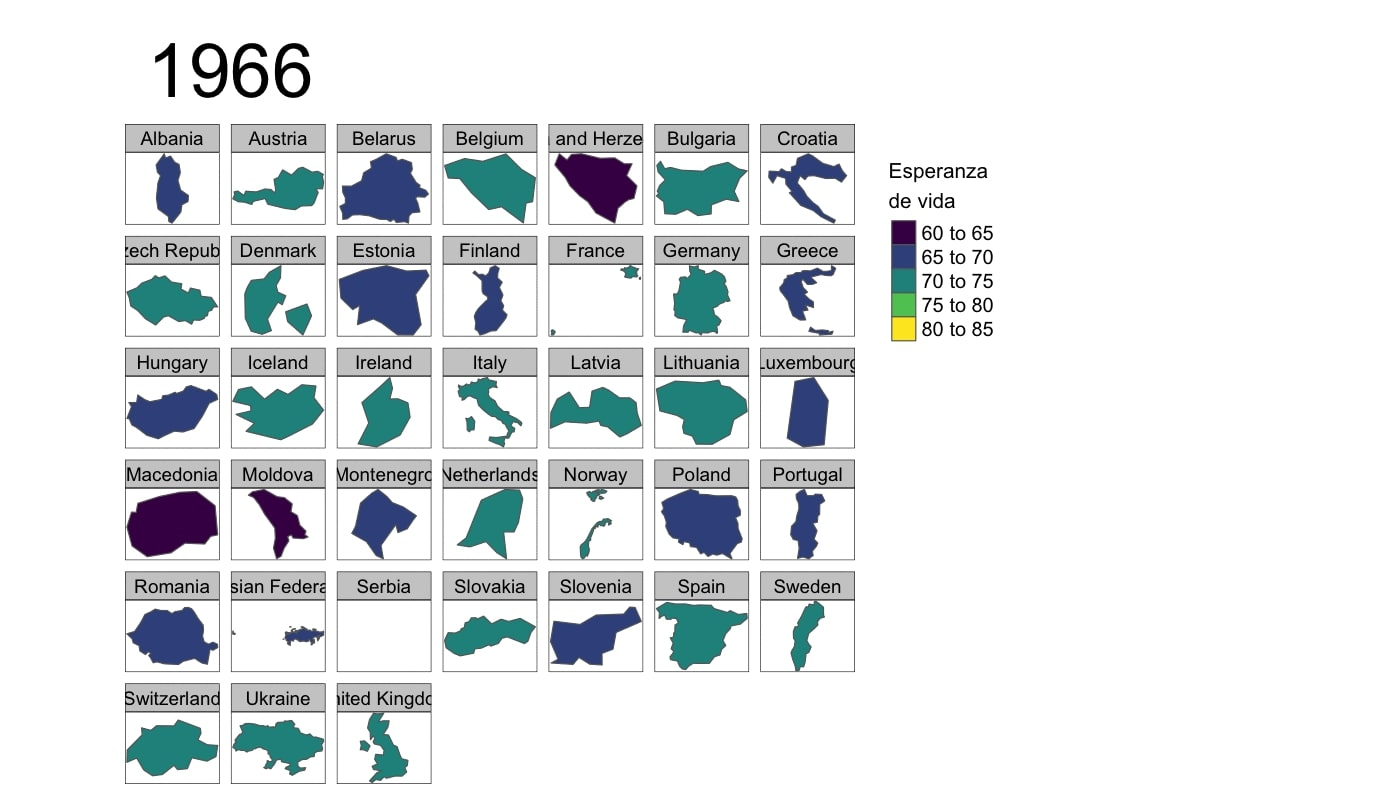
\includegraphics[width=0.77\textwidth]{Cap1/espvidaeur01.jpg}
\label{fig:subfig1}}
\subfloat{\hspace*{-4.05cm}
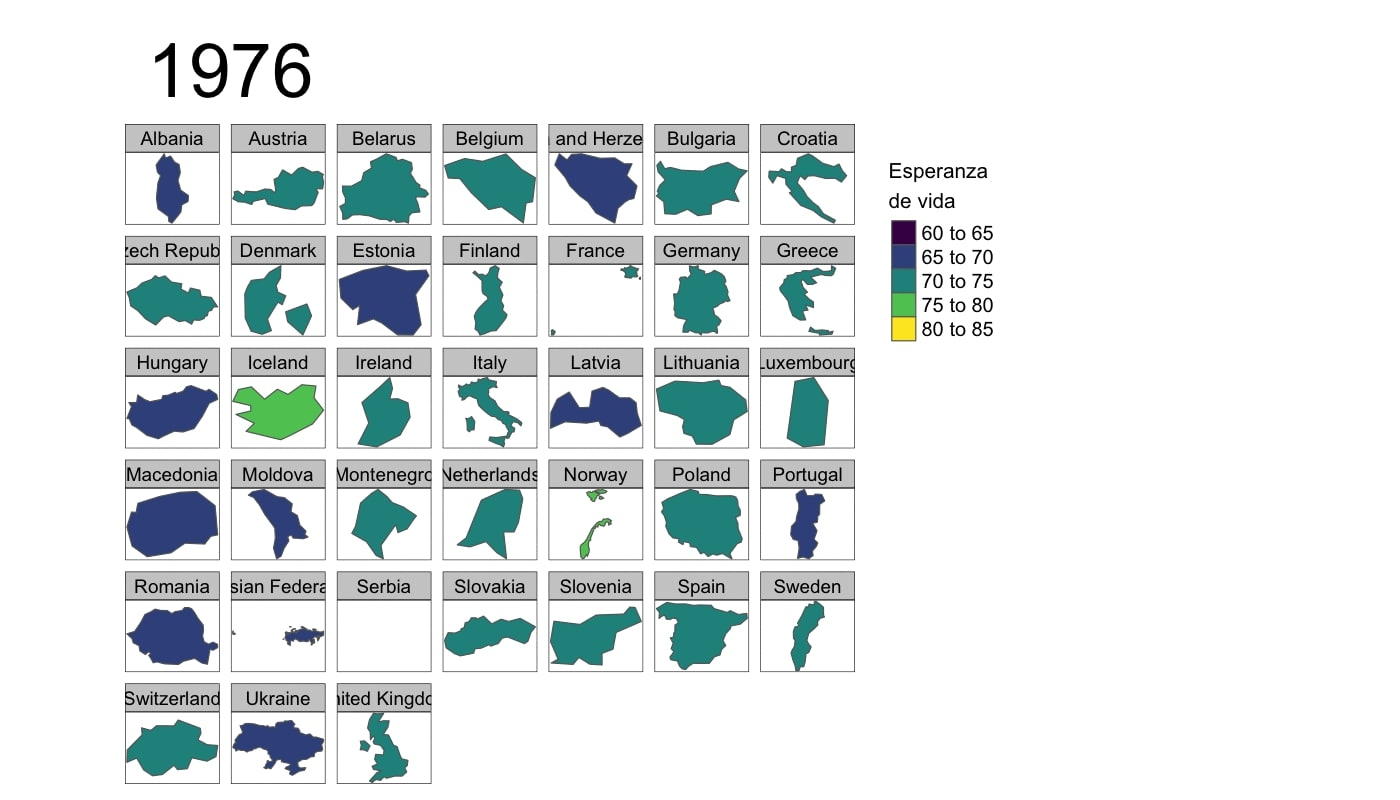
\includegraphics[width=0.77\textwidth]{Cap1/espvidaeur02.jpg}
\label{fig:subfig2}}
%\caption{This is a figure containing several subfigures.}
%\label{fig:globfig}
\end{figure}
\vspace{-1.4cm}
\begin{figure}[h]
\hspace*{-1.8cm}
\subfloat{
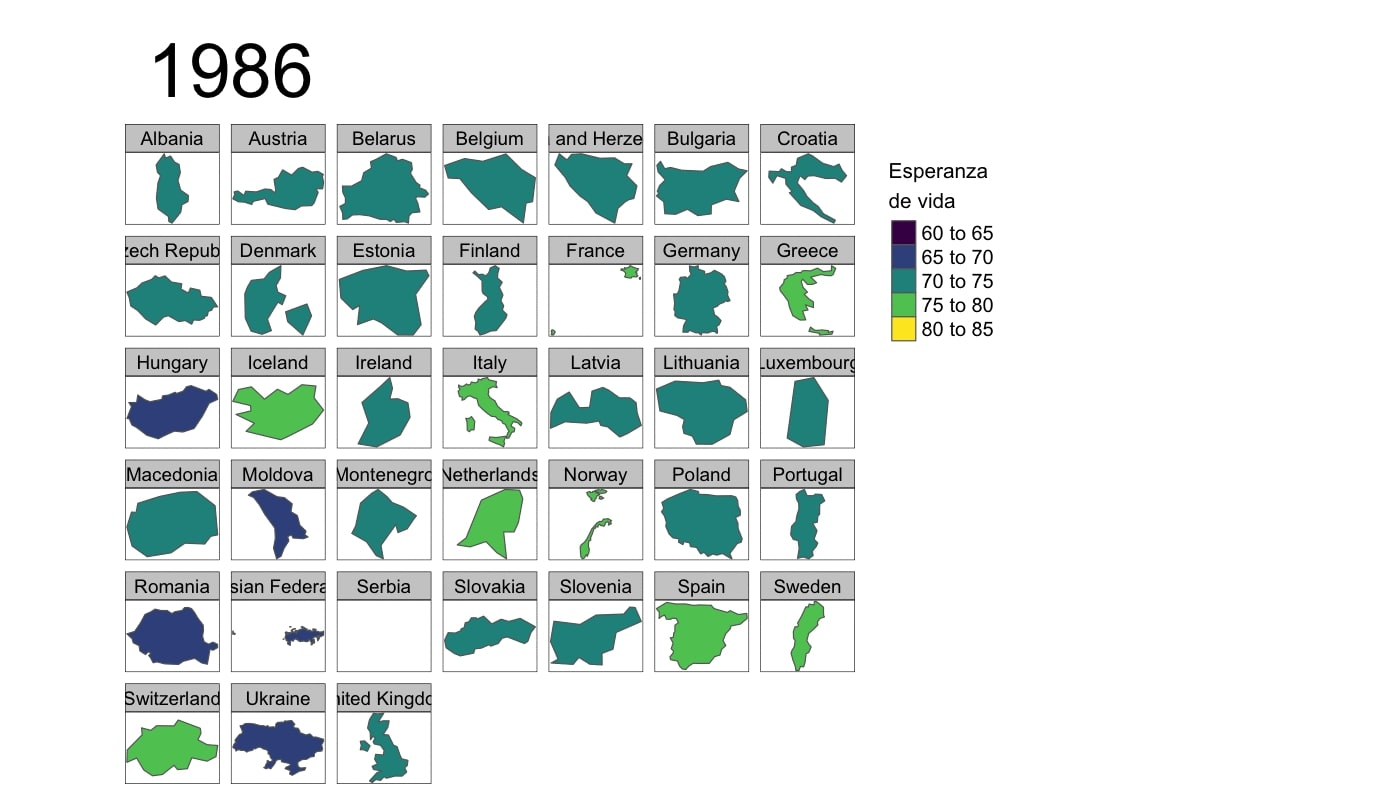
\includegraphics[width=0.77\textwidth]{Cap1/espvidaeur03.jpg}
\label{fig:subfig3}}
\subfloat{\hspace*{-4.05cm}
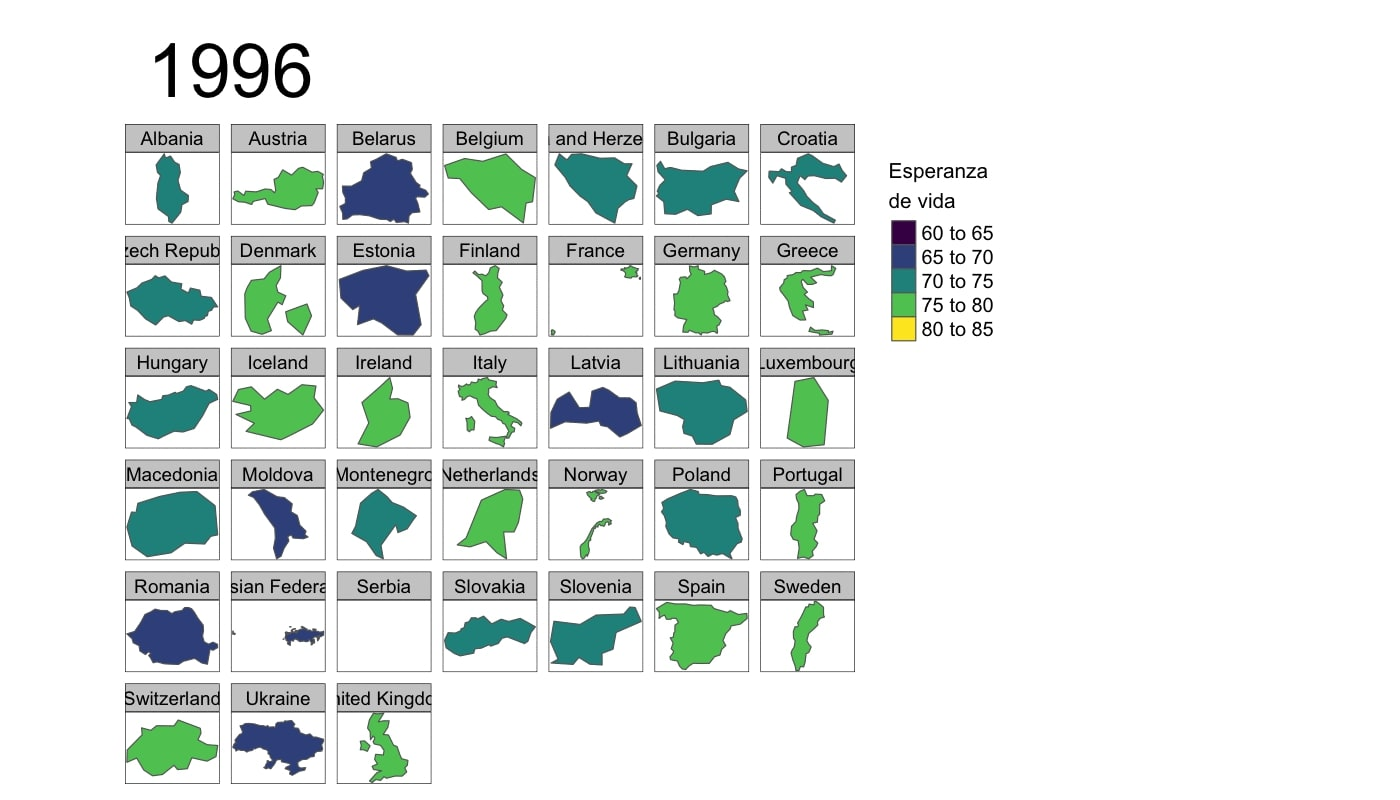
\includegraphics[width=0.77\textwidth]{Cap1/espvidaeur04.jpg}
\label{fig:subfig4}}
%\caption{This is a figure containing several subfigures.}
%\label{fig:globfig}
\end{figure}

\vspace{-1.2cm}
\begin{figure}[H]
\hspace*{-1.8cm}
\subfloat{
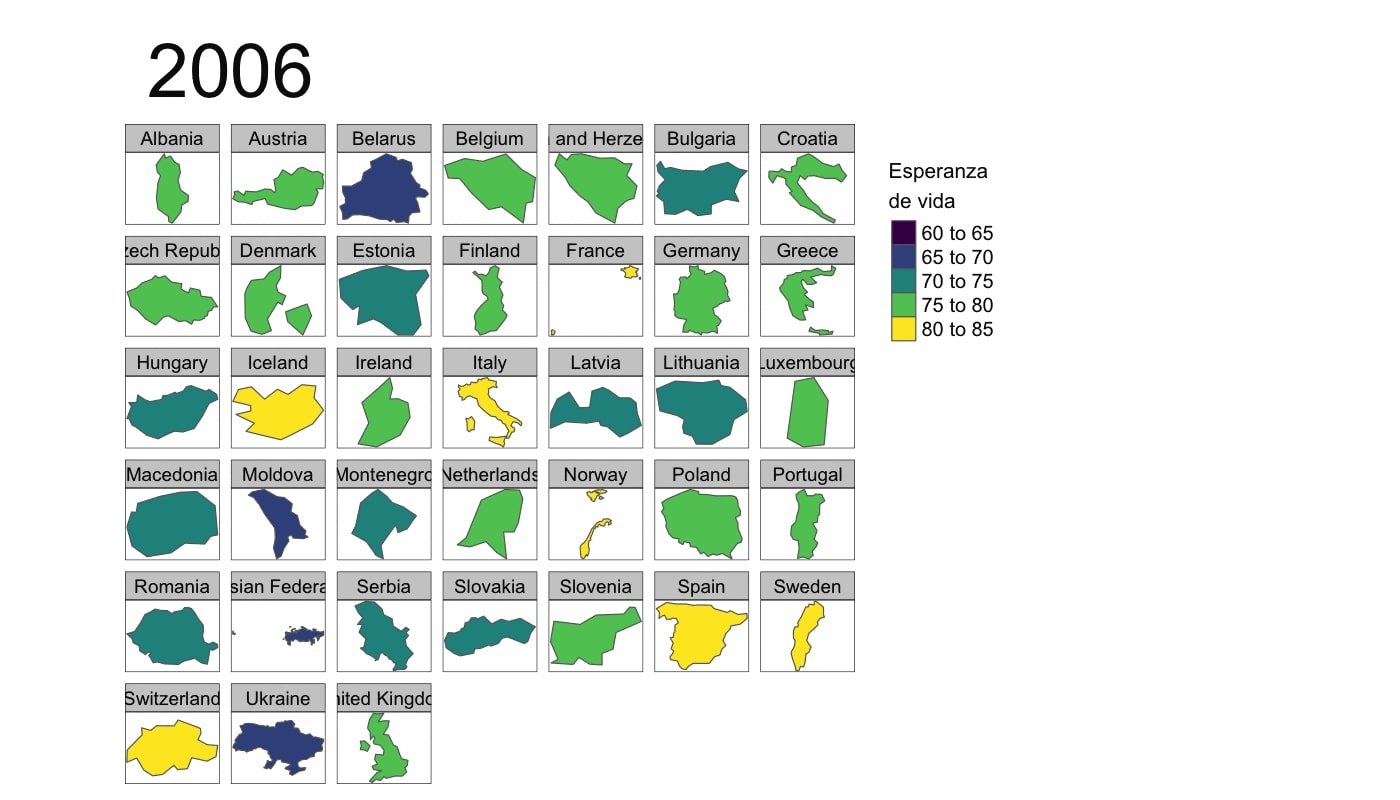
\includegraphics[width=0.77\textwidth]{Cap1/espvidaeur05.jpg}
\label{fig:subfig5}}
\subfloat{\hspace*{-4.051cm}
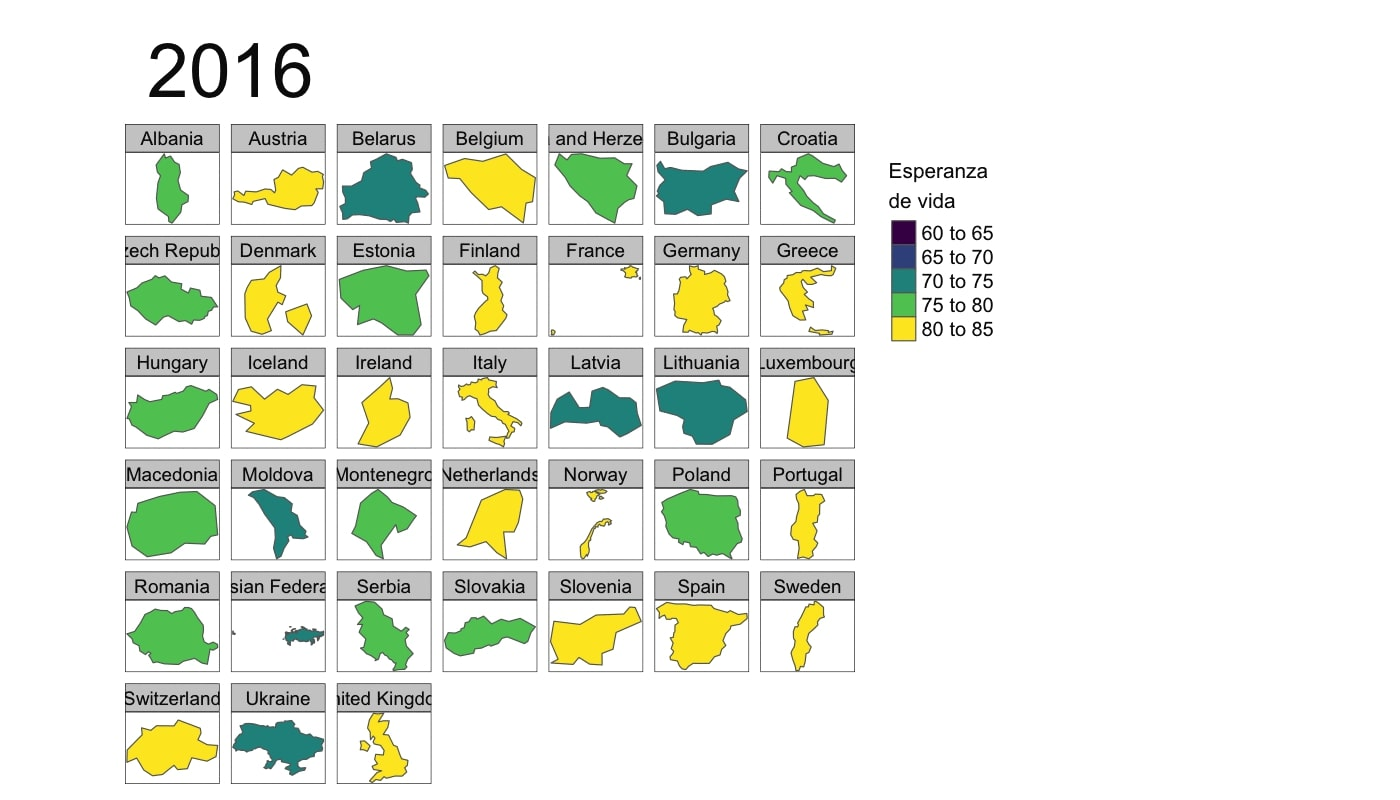
\includegraphics[width=0.77\textwidth]{Cap1/espvidaeur06.jpg}
\label{fig:subfig6}}
\vspace{-0.5cm}
\caption{Evolución de la esperanza de vida en los países europeos desde 1966.}\\
\hspace{4cm}\textit{\small{Fuente: Elaboración propia con \textbf{R} a partir de datos de Eurostat}}
\label{fig:globfig}
\end{figure}

\newpage
Si bien un aumento en la edad promedio es una tendencia común en todo el mundo, los factores que conducen a tales cambios varían según los países; se pueden remontar a disminuciones en las tasas de fertilidad y aumentos en la longevidad, aunque en diferentes magnitudes y en diferentes economías. Existen varios estudios que investigan cómo los factores institucionales y las respuestas de comportamiento pueden afectar el impacto del envejecimiento en la acumulación de capital; por ejemplo, Bloom y otros, (2007) \textcolor{red}{[22]}, señalan que las mejoras en una esperanza de vida saludable deberían generar aumentos en la edad media de jubilación, con poco efecto en el ahorro. Sin embargo, en muchos países, los incentivos de jubilación en los programas de seguridad social impiden que las edades de jubilación se mantengan a la par que los cambios en la esperanza de vida, lo que lleva a una mayor necesidad de ahorro en el ciclo de la misma.\\

Hemos visto que la población crecerá más lentamente, sí, pero no lo hará en todos los países de igual forma. Hemos señalado que la población envejecida crecerá; también, pero no crecerá en todos sitios de la misma manera (lo podemos ver en la figura 1.20) y hemos analizado que la población se volverá más urbana, pero no lo hará en todos los países igual.\\ 

Aunque en los próximos capítulos indagaremos en algunos aspectos matemáticos y estadísticos, no podemos olvidar la vertiente `social' de la demografía y del estudio de las poblaciones. Junto a una descripción de la situación actual y la explicación de algunos conceptos básicos, eso es lo que hemos intentado poner de manifiesto en este capítulo, que la demografía es algo más que un conjunto de técnicas y herramientas para predecir poblaciones, tasas de mortalidad y fertilidad, y ese `algo más' se relaciona sobre todo con la capacidad de los países para hacer frente la mencionada \textit{transición demográfica}; la adaptación del denominado \textit{Estado de Bienestar} a la creciente longevidad no es una tarea fácil; en tanto en cuanto los gobiernos de los países se erigen en garantes de ese estado, su mayor dificultad estriba en la existencia de significantes desigualdades entre los humanos en términos de longevidad, preferencias y racionalidad y para combatir estas desigualdades no es suficiente con las estadísticas, los promedios, las tasas de crecimiento, disminución, las simulaciones y las proyecciones. Cuando se trata de \textit{`adaptar el Estado de Bienestar'}, nos referimos al diseño de unas políticas óptimas en el contexto de preferencias y situaciones heterogéneas, y aunque tal desafío es una tarea ambiciosa, debería ser prioritaria en las agendas políticas de instituciones y gobiernos.\\

\newpage
\section*{Referencias bibliogr\'aficas}
\addcontentsline{toc}{section}{\protect\numberline{}Referencias bibliogr\'aficas}%

\noindent \textcolor{red}{[1]} Harper, Sarah: \textbf{``How Population Will Transform Our World''}, Oxford University Press, 1\textsuperscript{era} edici\'on, (2016).\\

\vspace{-0.23cm}
\noindent \textcolor{red}{[2]} Sartori, Giovanni y Mazzoleni, Gianni: \textbf{``La Tierra Explota: Superpoblaci\'on y Desarrollo''}, Ed. Taurus, (2003).\\

\vspace{-0.23cm}
\noindent \textcolor{red}{[3]} Ehrlich, Paul R. y Ehrlich Anne H.: \textbf{``La Explosi\'on Demogr\'afica''}, Ed. Salvat, 1\textsuperscript{era} edici\'on, (2003).\\

\vspace{-0.23cm}
\noindent \textcolor{red}{[4]} Ehrlich, Paul R.: \textbf{``The Population Bomb''}, Ballantines Books, 1\textsuperscript{era} edici\'on, (1968).\\

\vspace{-0.23cm}
\noindent \textcolor{red}{[5]} Leeson, George W.: \textbf{``C\'omo la Poblaci\'on Transformar\'a Nuestro Mundo''}, Vanguardia Dossier. Vol. 69, P\'ags. 6-13, (2018).\\

\vspace{-0.23cm}
\noindent \textcolor{red}{[6]} Kashnitsky, Ilya y Sch\"oley, Jonas: \textbf{``Regional Population Structures At a Glance''}, The Lancet Journal. Vol. 392, P\'ags. 209-210, (2018).\\

\vspace{-0.23cm}
\noindent \textcolor{red}{[7]} Tapinos, George: \textbf{``Elementos de Demograf\'ia''}, Ed. Espasa Universidad, (1990).\\

\vspace{-0.23cm}
\noindent \textcolor{red}{[8]} De Beer, Joop y otros: \textbf{``New Classification of Urban and Rural NUTS-2 Regions in Europe''}, Documento de trabajo del \textit{Netherlands Interdisciplinary Demographic Institute (NIDI)}, (2014).\\

\vspace{-0.23cm}
\noindent \textcolor{red}{[9]} González Martínez, C. I. y Conde-Ruíz, J. I.: \textbf{``España Ante el Reto de la Longevidad''}, \textit{Revista Actuarios}, n\textsuperscript{o} 42, (Primavera, 2018).\\

\vspace{-0.23cm}
\noindent \textcolor{red}{[10]} Vinuesa, Julio y otros (Coord.): \textbf{``Demograf\'ia. An\'alisis y Proyecciones''}, Ed. S\'intesis, (1997).\\

\vspace{-0.23cm}
\noindent \textcolor{red}{[11]} World Bank: \textbf{``Averting the Old Age Crisis: Policies to Protect the Old and Promote Growth}, \textit{World Bank Policy Research Report}, Ed. Oxford University Press, (1994).\\

\vspace{-0.23cm}
\noindent \textcolor{red}{[12]} Ayuso, Mercedes y Holzmann, Robert: \textbf{``Longevidad: un Breve An\'alisis Global y Actuarial''}, Documento de trabajo del \textit{Instituto BBVA de Pensiones}, (2014).\\

\vspace{-0.23cm}
\noindent \textcolor{red}{[13]} Citigroup: \textbf{``The Incoming Pension Crisis: Recommendations For Keeping the Global Pensions System Afloat''}, \textit{Citigroup Research}, (2018) [Disponible on line] \texttt{http://www.citi.com/citigps}.\\

\vspace{-0.23cm}
\noindent \textcolor{red}{[14]} Mackenback, Johan P: \textbf{``Changes in Mortality Inequalities Over Two Decades: Register Based Study of European Countries''}, \textit{British Medical Journal}, N\textsuperscript{o}353, (2016).\\

\vspace{-0.23cm}
\noindent \textcolor{red}{[15]} Raftery, Adrian E. y otros: \textbf{``Probabilistic Population Projections''}, \textit{Proceedings of the National Academy of Sciences}, (Agosto 2012), Vol. 109,  N\textsuperscript{o} 35, P\'ags. 13915-13921.\\
%; Li, Nan; \u{S}ev\u{c}\'ikov\`a, Hana; Gerland, Patrick y Heilig, Gerhard K.

\vspace{-0.23cm}
\noindent \textcolor{red}{[16]} Hansen, Alvin: \textbf{``Economic Progress and Declining Population Growth''}, AER, 29: 1-15 (1939).\\

\vspace{-0.23cm}
\noindent \textcolor{red}{[17]} Chesnais, Jean Claude: \textbf{``Economic Consecuences of Demographic Changes''}, Population and Developments: Challenges and Opportunities. UNESCO - Encyclopedia of Life Support System. (2013).\\

\vspace{-0.23cm}
\noindent \textcolor{red}{[18]} AIReF: \textbf{``Previsiones Demográficas: Una Visión Integrada''}, \textit{Documento Especial 2018/1}, Autoridad Independiente de Responsabilidad Fiscal, (octubre, 2018), \texttt{http://www.airef.es}\\

\vspace{-0.23cm}
\noindent \textcolor{red}{[19]} Dumont, G\'erard Francoise: \textbf{``Le Vieillissement Dans Le Monde: Cons\'equences G\'eopolitiques''}, Dossier Vanguardia, 69  (Julio/Septiembre 2018).\\

\vspace{-0.23cm}
\noindent \textcolor{red}{[20]} Botero, G.: \textbf{``On The Causes of the Greatness and Magnificence of Cities''}, \textit{editado por Luigi Ballerini y Massimo Ciavolella}. Ed. University of Toronto Press, (2012), JSTOR, \texttt{www.jstor.org/stable/\\10.3138/9781442665415}. \\

\vspace{-0.23cm}
\noindent \textcolor{red}{[21]} Pestieau, P. y Ponthierre, G.: \textbf{``Longevity Variations and the Welfare State''}, \textit{Journal of Demographic Economics}, 82, págs.: 207-239, (2016). \\

\vspace{-0.23cm}
\noindent \textcolor{red}{[22]} Bloom, D.; Canning, D.; y Moore, M.: \textbf{``A Theory of Retirement''}. NBER Working Papers 13630, (2007).\\


%Seg\'un la previsiones de la ONU, Espa\~na ser\'a el segundo pa\'is m\'as envejecido del mundo, detr\'as de Jap\'on, con el 41,9\% de la poblaci\'on de 60 o m\'as a\~nos en 2050. Su pir\'amide de edad, como la mayor\'ia de pa\'ises europeos, pasar\'a de piramidal a cil\'indrica. Se muestra, a continuaci\'on, una panor\'amica de la situaci\'on actual del pa\'is por lo que respecta a la poblaci\'on mayor, por municipios y autonom\'ias, en las que se indica las pensiones medias, adem\'as de la evoluci\'on y proyecciones de los principales datos demogr\'aficos, proporciones de poblaci\'on mayor y diferencias por sexo.

%\begin{figure}[H]
%\centering
%\hspace*{-1.2cm}
%\fbox{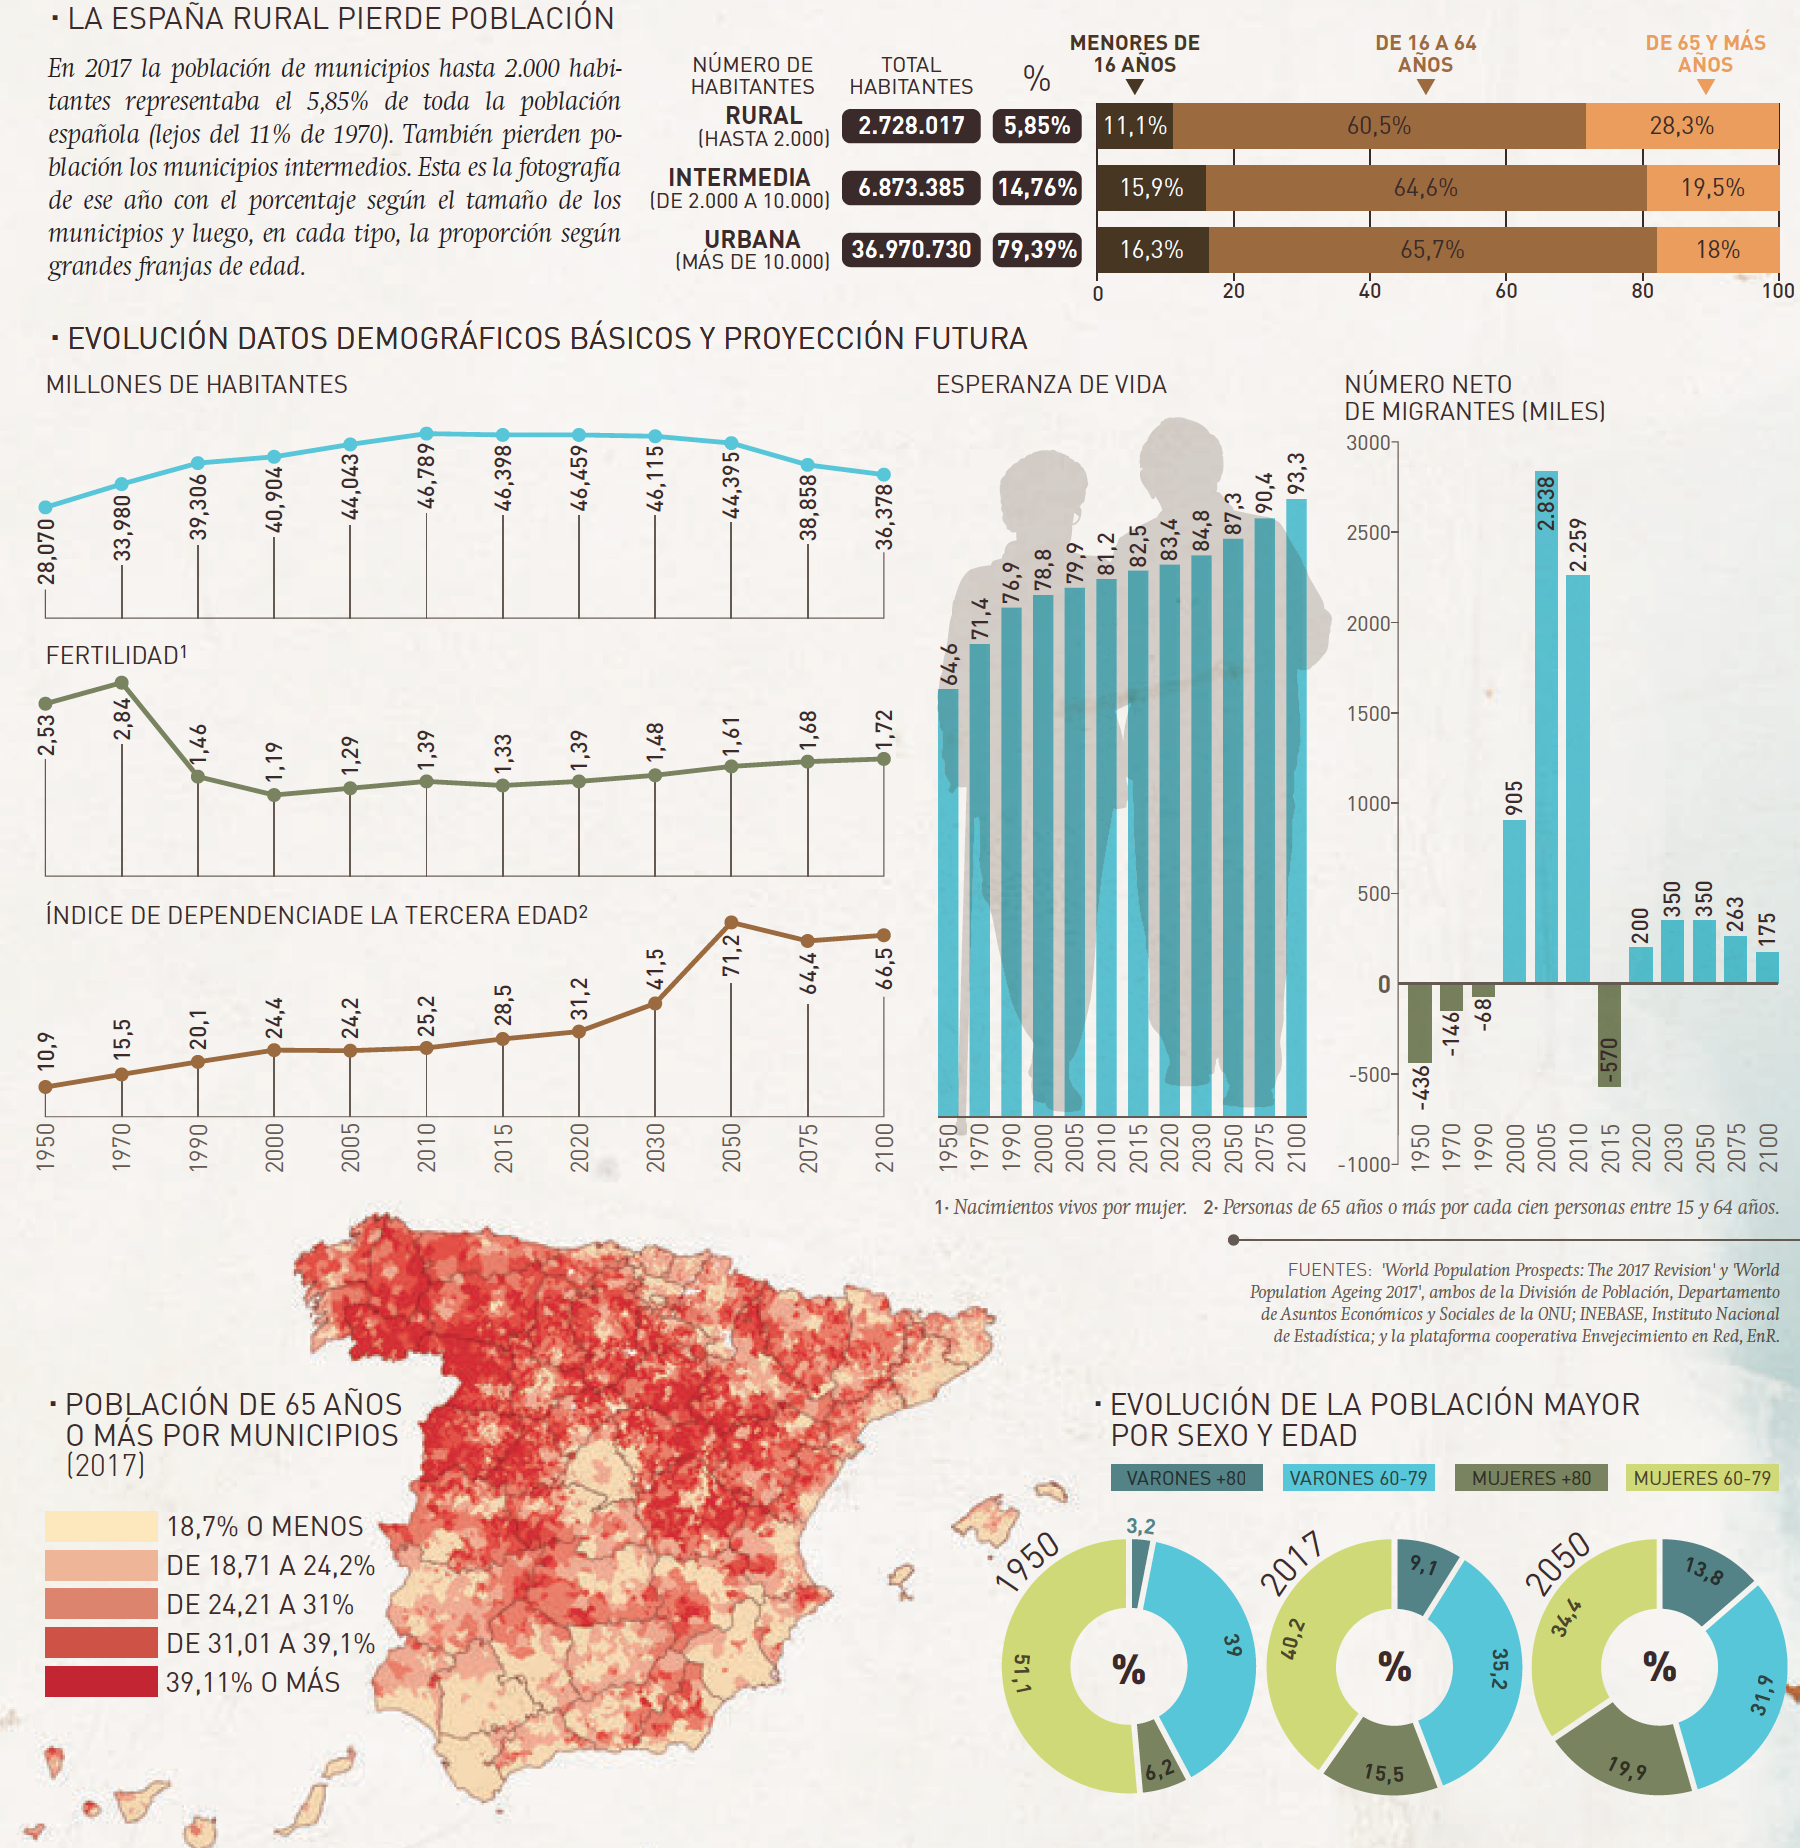
\includegraphics[scale=0.58]{Cap1/mayores1.png}}
%\caption{Estructuras de poblaci\'on regional}\\
%\textit{(Fuente: Eurostat)}
%\end{figure}
%\newpage
%\begin{figure}[!ht]
%\centering
%\hspace*{-0.65cm}
%\fbox{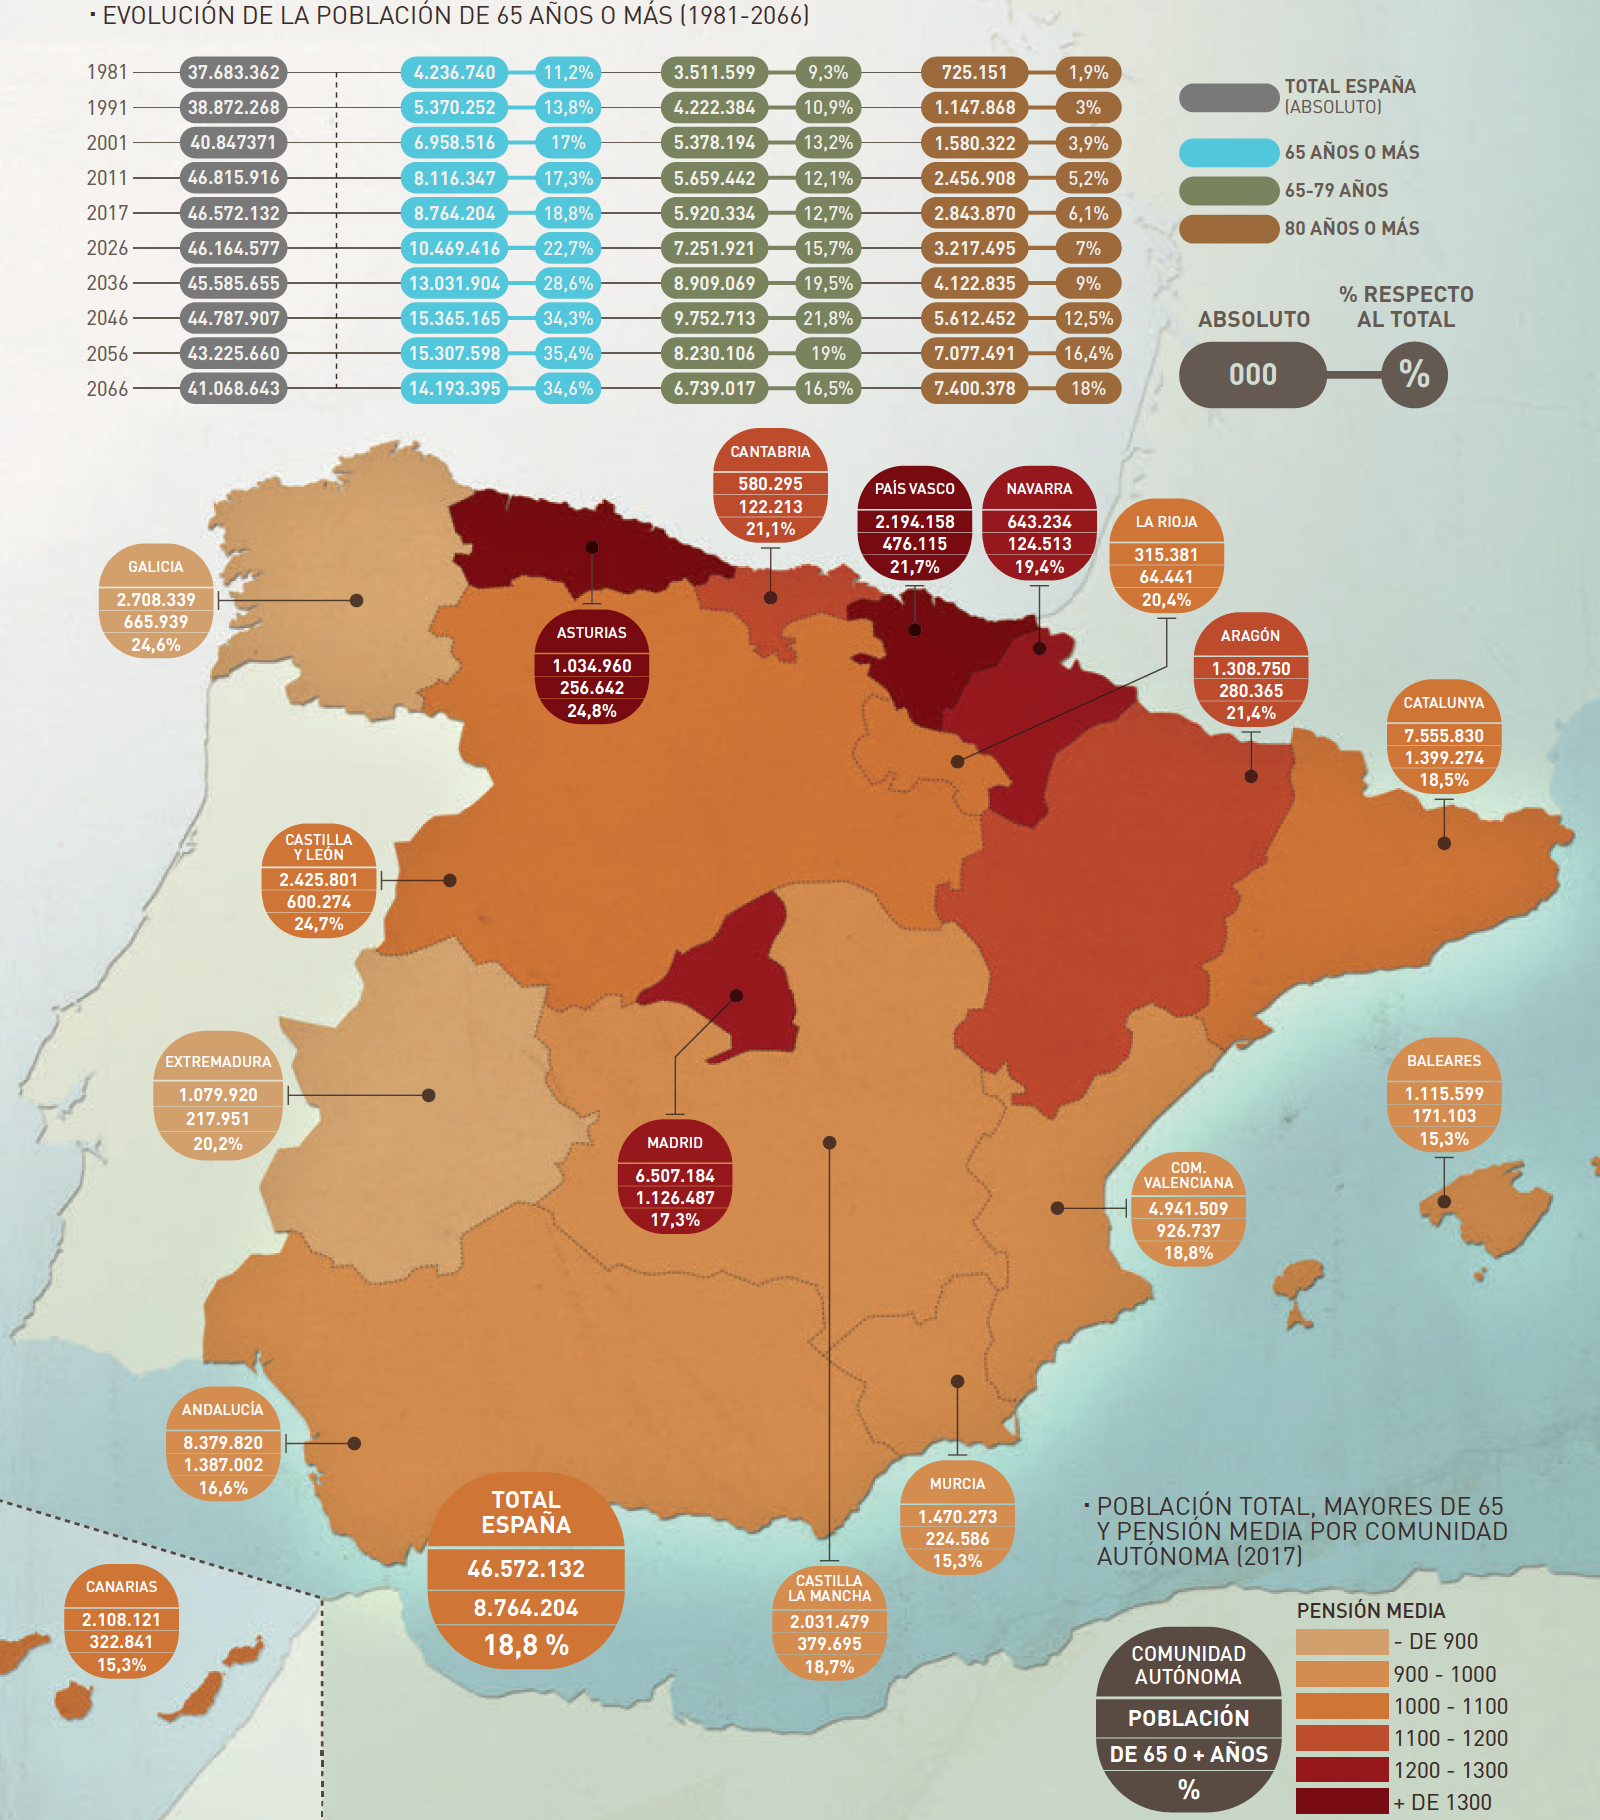
\includegraphics[scale=0.67]{Cap1/mayores2.png}}
%\caption{Estructuras de poblaci\'on regional}\\
%\textit{(Fuente: Eurostat)}
%\end{figure}

